\documentclass[10pt,a4paper,twoside]{report}

\usepackage{shika-bio}

\begin{document}

\begin{titlepage}

\begin{center}
	\textsc{{\Huge Shika Express - Biology}}\\[0.4cm]
	\textbf{{\huge Version 1.0 TZ}}\\[1.5cm]
	\HRule\\[0.4cm]
	\textsc{{\Large Hands-On Activities Companion Guide}}\\[0.4cm]
	\textsc{{\Large Tanzania}}\\[0.4cm]
	\HRule\\[0.5cm]
\end{center}

\vfill
\begin{center}
\textsc{{\Large Teacher's Guide}}\\[0.4cm]
\end{center}

% date at bottom
\begin{center}
	{\large \today}
\end{center}

\end{titlepage}

%\input{./tex/preface.tex}
%\input{./tex/background.tex}

\tableofcontents

% Biology Hands-On Activities
\clearpage
\phantomsection
\addcontentsline{toc}{part}{Hands-On Activities}
\part*{Hands-On Activities}
\settocdepth{subsection}

% Form I
\chapter{Biology Activities for Form I}
\section{Introduction to Biology}

\begin{multicols}{2}


\section*{Characteristics of Living \hfill \\ Things}


\subsection[Obvious Characteristics of Living Things]{Obvious Characteristics of \hfill \\ Living Things} % Source 10, LASM

\begin{center}
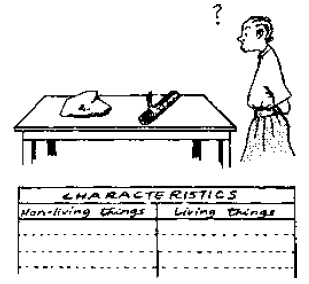
\includegraphics[width=0.45\textwidth]{./img/source/obv-char-living.png}
\end{center}

\begin{description*}
%\item[Subtopic:]{}
%\item[Materials:]{}
%\item[Setup:]{}
\item[Procedure:]{Display some non-living things such as a stone, piece of wood, glass of water etc., and list
any obvious differences between these things and a living organism (i.e. man). Produce a
table from the whole class response.}
%\item[Hazards:]{}
%\item[Questions:]{}
%\item[Observations:]{}
%\item[Theory:]{}
%\item[Applications:]{}
%\item[Notes:]{}
\end{description*}

\subsection{Other Characteristics of Living Things} % Source 11

\begin{center}
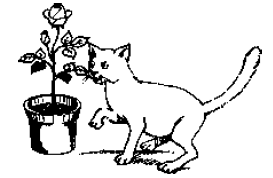
\includegraphics[width=0.4\textwidth]{./img/source/other-char-living.png}
\end{center}

\begin{description*}
%\item[Subtopic:]{}
%\item[Materials:]{}
%\item[Setup:]{}
\item[Procedure:]{Display a potted flowering plant and identify the main characteristics of life. Note that many
of these are less obvious in plants than in animals.}
%\item[Hazards:]{}
%\item[Questions:]{}
%\item[Observations:]{}
%\item[Theory:]{}
%\item[Applications:]{}
%\item[Notes:]{}
\end{description*}

\subsection{Is a Candle Living?} % Source 12

\begin{center}
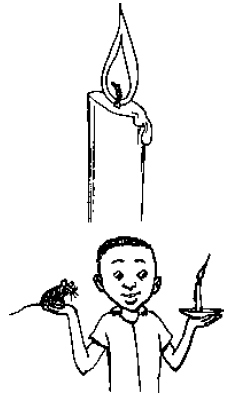
\includegraphics[width=0.4\textwidth]{./img/source/candle-living.png}
\end{center}

\begin{description*}
%\item[Subtopic:]{}
%\item[Materials:]{}
%\item[Setup:]{}
\item[Procedure:]{Look at a burning candle. The candle flame can be considered as an example of a process
in a state of dynamic equilibrium.}
%\item[Hazards:]{}
\item[Questions:]{What are the similarities and differences between a candle flame and a living organism.?}
%\item[Observations:]{}
\item[Theory:]{A candle flame is the result of a metabolic process. The candle wax is burnt to carbon
(soot) and other gaseous substances. The shape, colour and brightness of the flame remains
fairly constant, but only as long as there is a supply of wax and air. The flame is not selfsustained
and cannot reproduce itself.}
%\item[Applications:]{}
%\item[Notes:]{}
\end{description*}

%==================================================================================================%

\section*{Measurement in Biology}


\subsection{Data on Height} % Source 17

\begin{center}
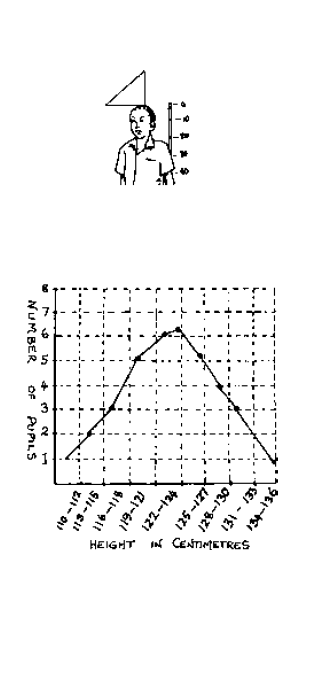
\includegraphics[width=0.45\textwidth]{./img/source/data-height.png}
\end{center}

\begin{description*}
%\item[Subtopic:]{}
%\item[Materials:]{}
%\item[Setup:]{}
\item[Procedure:]{Obtain the heights of all the student in the class (in centimetres). Use these heights to
divide the students into groups (i.e. 110-112 cms, 113-115 cms etc). Count the number of
pupils in each group. Plot a graph of height against numbers.}
%\item[Hazards:]{}
\item[Questions:]{What does the graph look like and what does this show?}
\item[Observations:]{A normal distribution curve is obtained showing that a few students are very tall, a few are
short, but most of them come somewhere between these extremes.}
\item[Theory:]{Members of a species can vary in size between a maximum and a minimum value, but
most individuals are near the middle of this range.}
%\item[Applications:]{}
%\item[Notes:]{}
\end{description*}

\vfill
\columnbreak

\subsection{Data on Pulse Rate}

\begin{center}
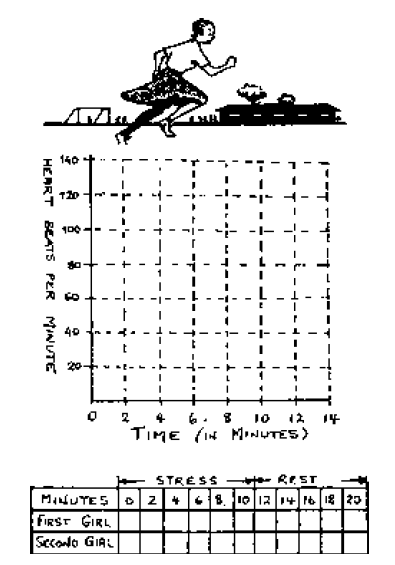
\includegraphics[width=0.4\textwidth]{./img/source/data-pulse.png}
\end{center}

\begin{description*}
%\item[Subtopic:]{}
%\item[Materials:]{}
%\item[Setup:]{}
\item[Procedure:]{Take the resting pulse rate of ten students, then ask them to run around the school
compound for two minutes. Take the pulse of each student at two minute intervals until the
pulse returns to normal. For each student plot a graph of pulse rate against time.}
%\item[Hazards:]{}
\item[Questions:]{Which pulse rate was the highest and which pulse returned to normal most quickly?}
\item[Observations:]{Each curve of pulse rate will be slightly different.}
\item[Theory:]{This is due to differences in levels of physical fitness of each student. The less fit ones
generally reach a higher pulse rate, which takes longer to return to normal.}
%\item[Applications:]{}
%\item[Notes:]{}
\end{description*}

\subsection{Measuring Growth}

\begin{center}
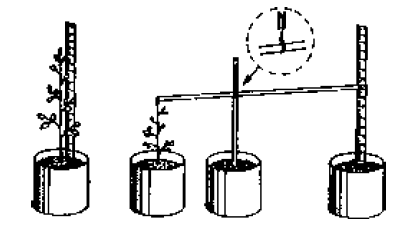
\includegraphics[width=0.4\textwidth]{./img/source/data-growth.png}
\end{center}

\begin{description*}
%\item[Subtopic:]{}
%\item[Materials:]{}
%\item[Setup:]{}
\item[Procedure:]{Take a seedling in a pot (or use a plant in its natural environment) and attach a fine thread
to a light stick (as shown above). Alternatively use the simple method for measuring growth.
Make measurements at fixed intervals (say 2 or 3 days). Devise a method of presenting your
data graphically.}
%\item[Hazards:]{}
%\item[Questions:]{}
%\item[Observations:]{}
%\item[Theory:]{}
%\item[Applications:]{}
%\item[Notes:]{}
\end{description*}

\subsection[Weight Increase by Germinating Seeds]{Weight Increase by \hfill \\ Germinating Seeds}

\begin{center}
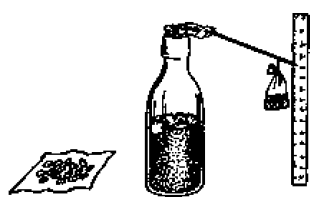
\includegraphics[width=0.45\textwidth]{./img/source/data-weight.png}
\end{center}

\begin{description*}
%\item[Subtopic:]{}
%\item[Materials:]{}
%\item[Setup:]{}
\item[Procedure:]{Place 10 bean seeds between pieces of wet newspaper. Place a second group of 10
beans between dry paper. Measure the weight of each group of beans at daily intervals, and
also record any observations.}
%\item[Hazards:]{}
\item[Questions:]{What are the differences in weight between the two groups of seeds?}
\item[Observations:]{The soaked beans swell and the weight increases. No change occurs in the beans on dry
paper.}
\item[Theory:]{The beans on the wet paper have absorbed water and started germinating. The dry beans
did not.}
%\item[Applications:]{}
%\item[Notes:]{}
\end{description*}

%\columnbreak

\subsection{Keeping a Written Record}

\begin{center}
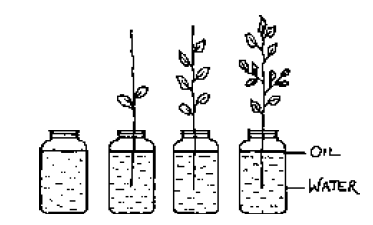
\includegraphics[width=0.45\textwidth]{./img/source/written-record.png}
\end{center}

\begin{description*}
%\item[Subtopic:]{}
%\item[Materials:]{}
%\item[Setup:]{}
\item[Procedure:]{Pick branches with different numbers of leaves and place each one in containers with the
same volume of water (To avoid loss by evaporation pour some oil on the surface). Record
the daily loss of water in each container.}
%\item[Hazards:]{}
%\item[Questions:]{}
\item[Observations:]{The more leaves on the branch, the greater the loss of water.}
\item[Theory:]{Leaves are the organs where most water is lost by the plant.}
%\item[Applications:]{}
%\item[Notes:]{}
\end{description*}

%==================================================================================================%

\section*{The Scientific Method}


\subsection{Transport of Water} % Source 17

\begin{center}
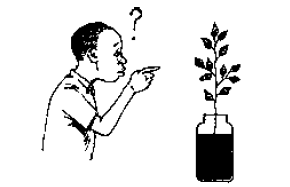
\includegraphics[width=0.45\textwidth]{./img/source/sci-meth-ink-plant.png}
\end{center}

\begin{description*}
%\item[Subtopic:]{}
%\item[Materials:]{}
%\item[Setup:]{}
\item[Hypothesis:]{Water is transported to the leaves where it is lost.}
\item[Procedure:]{Place a branch of a non woody plant in a solution of coloured ink.}
%\item[Hazards:]{}
%\item[Questions:]{}
\item[Observations:]{After some time the coloured ink is seen in the stem and leaves of the plant. A lot of liquid has been absorbed.}
\item[Conclusion:]{The plant transports water upwards through the stem to the leaves where most of
it is lost.}
%\item[Theory:]{}
%\item[Applications:]{}
%\item[Notes:]{}
\end{description*}

\subsection{Number of Leaves and Water Loss}

\begin{center}
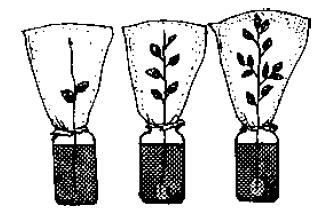
\includegraphics[width=0.4\textwidth]{./img/source/sci-meth-lose-water.png}
\end{center}

\begin{description*}
%\item[Subtopic:]{}
%\item[Materials:]{}
%\item[Setup:]{}
\item[Procedure:]{Using the same materials, place one plastic bag around a single leaf and
another around a branch with many leaves.}
%\item[Hazards:]{}
%\item[Questions:]{}
\item[Observations:]{More water collects in the bag enclosing the larger number of leaves.}
%\item[Theory:]{}
%\item[Notes:]{}
\item[Conclusion:]{Since water is lost from the leaves of a plant, the larger the number of leaves, the
greater the amount of water lost.}
\item[Applications:]{For better growth, plants need to be supplied with an adequate amount of water.
To reduce excessive water losses by transpiration, special methods of cultivation are used.}
%\item[Hypothesis:]{}
\end{description*}

%\subsection{Effect of Sunlight on Plant Growth}
%
%\begin{center}
%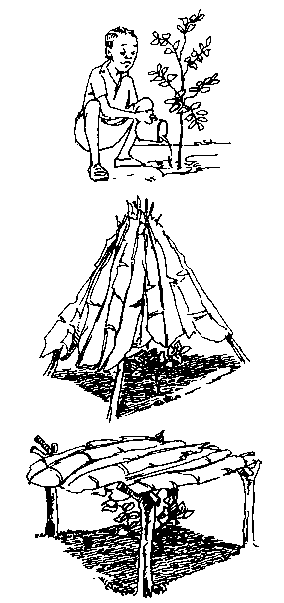
\includegraphics[width=0.4\textwidth]{./img/source/sci-meth-sun-water.png}
%\end{center}
%
%\begin{description*}
%%\item[Subtopic:]{}
%\item[Materials:]{}
%\item[Setup:]{}
%\item[Procedure:]{}
%\item[Hazards:]{}
%\item[Questions:]{}
%\item[Observations:]{}
%\item[Theory:]{}
%\item[Applications:]{}
%\item[Notes:]{}
%\item[Conclusion:]{}
%\item[Hypothesis:]{}
%\end{description*}

\vfill
\pagebreak

%==================================================================================================%



\end{multicols}


\subsection{Hand Washing}

%\begin{center}
%\includegraphics[width=0.4\textwidth]{./img/source/.jpg}
%\end{center}

\begin{description*}
\item[Materials:]{Soap, water, bottle, basin/bucket, chalk, charcoal, food colour, stopwatch}
\item[Setup:]{Prepare a large amount of soapy water. Grind the chalk and charcoal into separate powders.}\\
\item[Problem:]{How long should we wash our hands?\\

\begin{tabular}{|l|c|c|} \hline
\multirow{2}{*}{\textbf{Material}} & \textbf{Hypothesis} & \multirow{2}{*}{\textbf{Experimental Result}} \\
& \textbf{(Seconds)} & \\ \hline
Chalk powder & & \\ \hline
Charcoal powder & & \\ \hline
Food colour & & \\ \hline
\end{tabular} \\[10pt]
}\\
\item[Hypothesis:]{Predict how much time it will take to completely clean your hands and record in the table.}
\item[Procedure:]{Start a stopwatch and have a student or teacher slowly pour soapy water over a basin while the student washes his or her hands. Stop the clock when the student's hands are completely clean.}
\item[Observations:]{Record the time taken to completely wash your hands in the table.}
\item[Questions:]{}\hfill
\begin{enumerate}
\item Why is it important to wash our hands?
\item When do we need to wash our hands?
\end{enumerate}
\item[Theory:]{Washing our hands with soap and water helps to kill harmful bacteria that can cause us to become sick if allowed into our bodies. It is very important to wash our hands before eating and after using the bathroom.}
\end{description*}

\pagebreak


\subsection{Lung Capacity}

\begin{center}
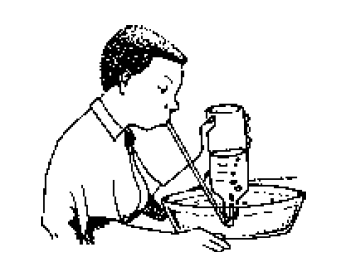
\includegraphics[width=0.4\textwidth]{./img/source/lung-capacity.png}
\end{center}

\begin{description*}
\item[Materials:]{1.5 L bottle, basin, water, plastic tubes/straws, soap, marker, ruler}
\item[Setup:]{Make a scale on the bottle using a marker and ruler (e.g. 100 mL increments). Prepare a soap solution for washing the tubes/straws}\\
\item[Problem:]{How much air can your lungs hold?\\

\begin{tabular}{|l|c|c|} \hline
\multirow{2}{*}{\textbf{Breath}} & \textbf{Hypothesis} & \multirow{2}{*}{\textbf{Experimental Result}} \\
& \textbf{(Volume of air in mL)} & \\ \hline
Normal breath & & \\ \hline
Full breath & & \\ \hline
After holding breath for 10 seconds & & \\ \hline
\end{tabular} \\[10pt]
}
\item[Hypothesis:]{Record the volume of air that you think the lungs can hold for each case in the table.}
\item[Procedure:]{Fill a basin with water. Fill a 1.5 L bottle with water and invert it in the basin so that the mouth of the bottle is underneath the water. Place one end of the tube/straw inside the bottle under water. For each breath, blow into the tube to displace the water.}
\item[Observations:]{Note the reading on the scale before and after blowing into the tube and record the \emph{difference} to give the amount of water displaced.}
\item[Questions:]{}\hfill
\begin{enumerate}
\item Which breath produces the largest amount of air? Which give the smallest amount?
\item How long can you hold your breath?
	\begin{enumerate}
	\item[] Hypothesis: I can hold my breath for \_\_\_\_\_\_\_ seconds.
	\item[] Experimental Result: I can hold my breath for \_\_\_\_\_\_\_ seconds.
	\end{enumerate}
\end{enumerate}
\item[Theory:]{When we breath in air, our bodies use the oxygen and produce carbon dioxide in a process called \emph{respiration}. Oxygen is transported in our blood throughout our bodies. When we hold our breath, oxygen is not circulated throughout our bodies and we begin to feel lightheaded.}
\end{description*}




%\vfill
\pagebreak
\section{Safety in Our Environment}

\begin{multicols}{2}


\section*{Waste Disposal}


\subsection{Biodegradable Waste} % banana, bottle, etc in a hole

%\begin{center}
%\includegraphics[width=0.4\textwidth]{./img/.png}
%\end{center}

\begin{description*}
%\item[Subtopic:]{}
\item[Materials:]{Shovel/jembe, Banana peel, plastic bottle, rubber bands, paper}
%\item[Setup:]{}
\item[Procedure:]{Dig several small holes and place a different item in each, covering them with dirt. Check back on the items after several weeks, months, and after a year.}
%\item[Hazards:]{}
%\item[Questions:]{}
\item[Observations:]{The banana peel shrivels and degrades after a couple weeks, while the other items remain for many months or even years.}
\item[Theory:]{Banana peels are an example of organic waste. They are \emph{biodegradable}}, meaning that it breaks down in the environment. \emph{Non-biodegradable} waste does not break down, it just piles up.
\item[Applications:]{Do not throw plastic bottles out of the window on buses!!}
%\item[Notes:]{}
\end{description*}

\vfill
\columnbreak

\subsection{Trash Journal} % Shika 242 

%\begin{center}
%\includegraphics[width=0.4\textwidth]{./img/.png}
%\end{center}

\begin{description*}
%\item[Subtopic:]{}
%\item[Materials:]{}
%\item[Setup:]{}
\item[Procedure:]{Have each student record in a journal all of the trash that they make every day for 2 weeks. If possible, collect the trash and weigh it every day.}
%\item[Hazards:]{}
\item[Observations:]{}
\item[Theory:]{Trash is a big problem in large towns and cities. Many manufactured goods come with a lot of waste material, which accumulates over time. Many waste items can be \emph{recycled}, or reused for different purposes.}
\item[Questions:]{What are some methods for eliminating waste? What effect does burning trash have on the environment?}
%\item[Applications:]{}
%\item[Notes:]{}
\end{description*}

%==================================================================================================%


\end{multicols}
\vfill
\pagebreak
\section{Health and Immunity}

\begin{multicols}{2}


\subsection{Coughs and Sneezes Spread Diseases} % VSO 58, Source 121

\begin{center}
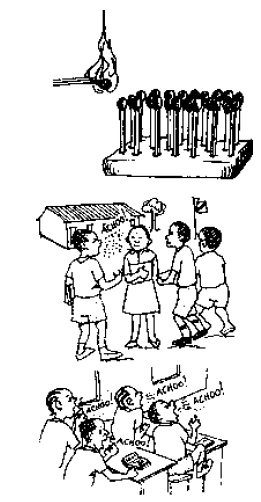
\includegraphics[width=0.4\textwidth]{./img/source/coughs.png}
\end{center}

\begin{description*}
%\item[Subtopic:]{}
%\item[Materials:]{}
%\item[Setup:]{}
\item[Procedure:]{Place the matches in the match box as shown and ignite one.}
%\item[Hazards:]{}
\item[Questions:]{Why is it dangerous to sneeze or cough without covering the mouth or nose?}
%\item[Observations:]{}
\item[Theory:]{Moisture may be seen leaving an uncovered mouth or nose. The water droplets contain
microbes. If one is suffering from an airborne disease such as influenza or tuberculosis
sneezing or coughing could be a source of spreading the harmful microbes. It is necessary to
be aware of this when coughing/sneezing, so that we do not spread the germs to others.
}
\item[Applications:]{Doctors and nurses wear masks to stop germs from their noses and mouths getting on to
people having operations or on to newborn babies.}
%\item[Notes:]{}
\end{description*}

\subsection{Smoking and Health}

\begin{center}
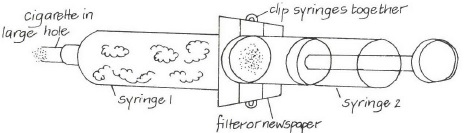
\includegraphics[width=0.45\textwidth]{./img/vso/smoking.jpg}
\end{center}

\begin{description*}
%\item[Subtopic:]{}
\item[Materials:]{2 syringes, filter paper, cigarette}
%\item[Setup:]{}
\item[Procedure:]{Remove the needle end from one syringe (syringe 2). Remove the
plunger from the other syringe (syringe 1) and make a larger hole in
the needle end. Join the syringes as shown. Place a piece of filter paper
or newspaper between the 2 syringes. Place the cigarette in syringe 1
and light it. Draw air through the cigarette several times.}
%\item[Hazards:]{}
\item[Observations:]{You will
see a dark stain spreading across the filter paper. This is tar from the cigarette.}
\item[Questions:]{Ask students what happens to the tar if a person smokes the cigarette and discuss its effect on health.}
%\item[Theory:]{}
%\item[Applications:]{}
%\item[Notes:]{}
\end{description*}

\subsection{Water Baby} % VSO 58

\begin{center}
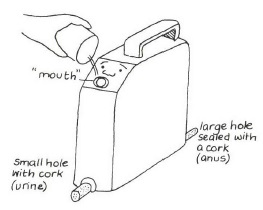
\includegraphics[width=0.4\textwidth]{./img/vso/water-baby.jpg}
\end{center}

\begin{description*}
%\item[Subtopic:]{}
\item[Materials:]{Plastic bottle, 2 corks, water}
%\item[Setup:]{}
\item[Procedure:]{Make a model baby from the bottle. The hole in the top
represents the mouth. Make
a small hole at the bottom to represent water loss through urine and a large hole
to represent the anus. Put corks in both holes. Fill the `baby' with
water. }
%\item[Hazards:]{}
%\item[Questions:]{}
\item[Observations:]{Remove the smaller plug and
water will be lost slowly.
However, diarrhea can cause
severe loss of water, as removing
the larger plug illustrates. }
\item[Theory:]{Water
lost through the holes can only be
replaced through the `mouth'. lf more water is lost than is taken in dehydration occurs and this can
be fatal especially in small babies.}
%\item[Applications:]{}
%\item[Notes:]{}
\end{description*}

\subsection{Oral Rehydration Solution}

\begin{center}
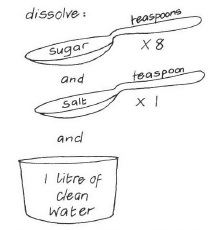
\includegraphics[width=0.4\textwidth]{./img/vso/ors.jpg}
\end{center}

\begin{description*}
%\item[Subtopic:]{}
\item[Materials:]{1 L clean water, 8 teaspoons sugar, 1 teaspoon salt}
%\item[Setup:]{}
\item[Procedure:]{Combine the materials to make an Oral Rehydration Solution (ORS) to help treat diarrhea.}
%\item[Hazards:]{}
%\item[Questions:]{}
%\item[Observations:]{}
\item[Theory:]{Our bodies need water to function normally,
but we also need a particular concentration of essential electrolytes,
e.g. sodium and potassium. These electrolytes are lost in diarrhea and
they must be replaced. Drinking water alone will not save the life of a
person who is dehydrated and has lost too many electrolytes. To
replace some essential electrolytes and water, the baby, or adult,
should drink the Oral Rehydration Solution (ORS)
shown here.}
%\item[Applications:]{}
\item[Notes:]{This is an emergency solution and does not contain
all electrolytes. A severely dehydrated baby may need a
more complex solution if diarrhea persists.}
\end{description*}

\subsection{HIV Acting} % VSO 59

\begin{center}
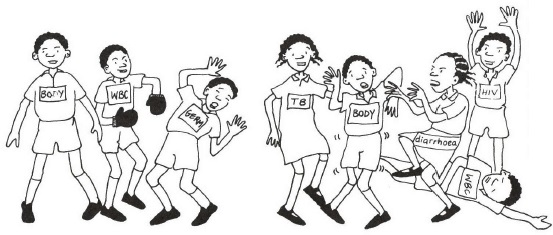
\includegraphics[width=0.4\textwidth]{./img/vso/hiv-acting.jpg}
\end{center}

\begin{description*}
%\item[Subtopic:]{}
\item[Materials:]{Cards, pins/tape}
%\item[Setup:]{}
\item[Procedure:]{Make cards to attach to students. They should contain a mixture of the
following - HIV; diseases, e.g. TB, diarrhea; white blood cell. One of
the pupils should represent the human body. Several `white blood cells'
should be protecting one body' to begin with. Ask students to act out
the spread of HlV.}
%\item[Hazards:]{}
%\item[Questions:]{}
%\item[Observations:]{}
\item[Theory:]{White blood cells protect the
body from diseases. HIV knocks
out the white blood cells and so
they can no longer protect the
body. This leaves the body open
to attack by germs of all kinds.
Eventually the body is overcome
by diseases which are normally
not fatal.}
%\item[Applications:]{}
%\item[Notes:]{}
\end{description*}

\subsection{Passing On HIV}

\begin{center}
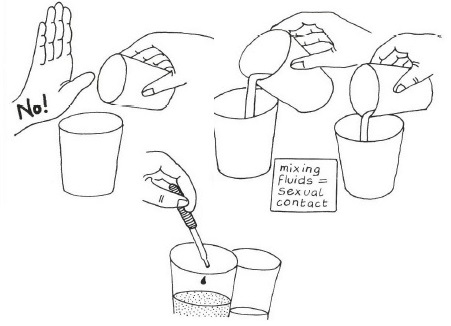
\includegraphics[width=0.4\textwidth]{./img/vso/hiv-passing.jpg}
\end{center}

\begin{description*}
%\item[Subtopic:]{}
\item[Materials:]{Cards, starch solution, iodine solution}
\item[Setup:]{On the cards write down some sexual case histories. Give each student
a card at random. The owner of the card is to follow the behaviour
indicated on the card, e.g. faithful to one partner, many partners, no
partners. }
\item[Procedure:]{Give a few of the students a cup of starch solution and give
all the others a cup of water. Ask students to follow the case history of
the cards and to mix the contents of their cups when they have a
partner - mixing represents sexual contact. At some point `HlV test' the
contents of the cups using a few drops of iodine solution. lf the
solution goes dark then it means there is starch (representing HIV) in
the cup.}
%\item[Hazards:]{}
%\item[Questions:]{}
\item[Observations:]{Discuss how fast the virus
spreads. Also discuss how its
spread could be prevented or
slowed down.}
%\item[Theory:]{}
%\item[Applications:]{}
%\item[Notes:]{}
\end{description*}

%==================================================================================================%


\end{multicols}

\pagebreak
\section{Cell Structure and Organization} \index{Cells! structure and organization}

\begin{multicols}{2}


%\section*{}


\subsection{Cells, Tissues, Organs} % VSO 22

\begin{center}
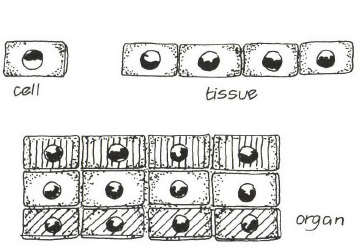
\includegraphics[width=0.49\textwidth]{./img/vso/cells-tissues-organs.jpg}
\end{center}

\begin{description*}
%\item[Subtopic:]{}
\item[Materials:]{Matchboxes, peas/beans/stones, boxes of different colour or size}
%\item[Setup:]{}
\item[Procedure:]{Place a seed in each box. This represents the nucleus: the matchbox the
cell. Place groups of cells inside the coloured boxes - the different
coloured boxes represent different tissues and the boxes themselves
can be joined to make organs.}
%\item[Hazards:]{}
%\item[Questions:]{}
%\item[Observations:]{}
%\item[Theory:]{}
\item[Applications:]{The school is a useful model of an organism. The bricks (cells) make
walls (tissues) and walls make classrooms (organs). The corridors can
therefore be used as models for transport systems.
}
\item[Notes:]{Another analogy might be a town where buildings represent organs,
rooms the tissues or cells and people inside the rooms the various
functions of the cell.}
\end{description*}

\subsection{Cell Models}

\begin{center}
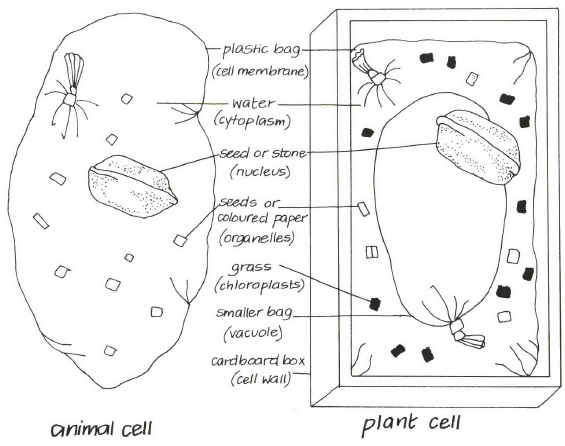
\includegraphics[width=0.49\textwidth]{./img/vso/cell-models.jpg}
\end{center}

\begin{description*}
%\item[Subtopic:]{}
\item[Materials:]{2 large and 2 small plastic bags, water, 2 large seeds/stones, small seeds/coloured paper, grass, cardboard box}
%\item[Setup:]{}
\item[Procedure:]{Make models of plant and animal cells as shown.}
%\item[Hazards:]{}
%\item[Questions:]{}
%\item[Observations:]{}
%\item[Theory:]{}
%\item[Applications:]{}
%\item[Notes:]{}
\end{description*}

\subsection{Looking at Cells} % VSO 23

\begin{center}
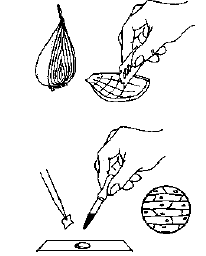
\includegraphics[width=0.35\textwidth]{./img/source/looking-cells.png}
\end{center}

\begin{description*}
%\item[Subtopic:]{}
\item[Materials:]{Onion, pin/needle, glass, plastic strip, iodine solution}
%\item[Setup:]{}
\item[Procedure:]{Cut a slice of onion and gently
peel off a piece of the thin inner
surface skin layer. With a
pin/needle place a piece of `skin'
in a water drop on a piece of
glass. Stain the `skin' with a drop
of iodine solution. Lower a cover
slip (plastic strip) onto the specimen taking care
not to let in any air bubbles.
Now view the prepared
slide through the microscope.}
%\item[Hazards:]{}
%\item[Questions:]{}
%\item[Observations:]{}
%\item[Theory:]{}
%\item[Applications:]{}
%\item[Notes:]{}
\end{description*}

\subsection{How Many Cells?} % VSO 23

%\begin{center}
%\includegraphics[width=0.4\textwidth]{./img/.png}
%\end{center}

\begin{description*}
%\item[Subtopic:]{}
%\item[Materials:]{}
%\item[Setup:]{}
\item[Procedure:]{Ask students to estimate how many cells there are in the human body. How many grains of sand would fit in the human body? Have students make a dot with a sharp pencil.}
%\item[Hazards:]{}
%\item[Questions:]{}
%\item[Observations:]{}
\item[Theory:]{A grain of sand is several thousand times larger than a human cell. Even the largest human cell, the ovum, is smaller than the pencil dot.}
%\item[Applications:]{}
%\item[Notes:]{}
\end{description*}

\columnbreak

\subsection{Simple Microscope} \index{Microscope} % VSO 23

\begin{center}
%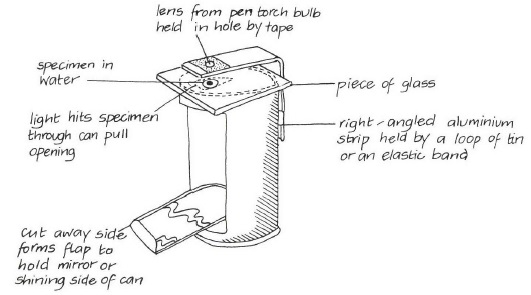
\includegraphics[width=0.49\textwidth]{./img/vso/microscope.jpg}
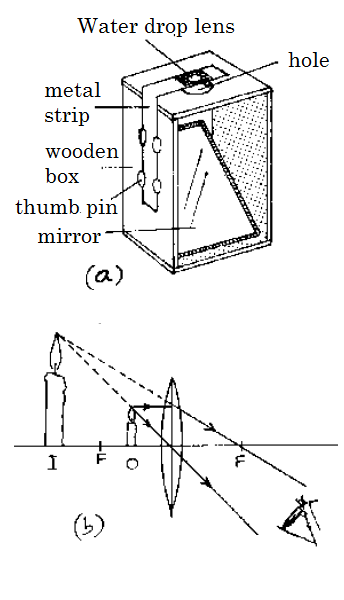
\includegraphics[width=0.49\textwidth]{./img/source/simple-microscope.png}
\end{center}

\begin{description*}
%\item[Subtopic:]{}
\item[Materials:]{Soda can, small lens (e.g. pen-torch bulb), aluminium strip, small mirror, piece of glass, rubber band}
%\item[Setup:]{}
\item[Procedure:]{Make the microscope as shown.
Some care is needed in
positioning the lens in the hole
made for it in the aluminium
strip. The inside of the can may be
painted black. Such a microscope
is quite adequate for looking at
cells.}
%\item[Hazards:]{}
%\item[Questions:]{}
%\item[Observations:]{}
%\item[Theory:]{}
%\item[Applications:]{}
%\item[Notes:]{}
\end{description*}

\vfill
\columnbreak

\subsection{Cell Size}

\begin{center}
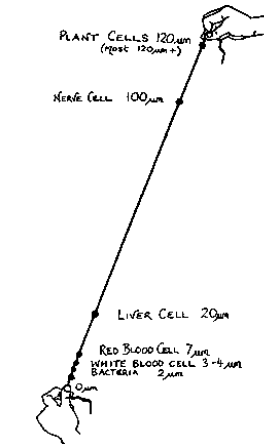
\includegraphics[width=0.4\textwidth]{./img/source/cell-size.png}
\end{center}

\begin{description*}
%\item[Subtopic:]{}
\item[Materials:]{String/chalk}
%\item[Setup:]{}
\item[Procedure:]{Take a piece of string (or chalk a line on the ground) about 60 cm long. Mark distances as
shown in the diagram above. The lengths represent the sizes of different types of cells
enlarged one thousand times.}
%\item[Hazards:]{}
\item[Questions:]{How many times bigger is a plant stem cell than a blood cell?}
\item[Observations:]{50 times.}
\item[Theory:]{Although almost all cells are too small to be seen with the unaided eye, they show a wide
range of sizes (about the same range as a mouse and an elephant).}
%\item[Applications:]{}
%\item[Notes:]{}
\end{description*}

%==================================================================================================%


\end{multicols}

\pagebreak
\section{Classification of Living Things}

\begin{multicols}{2}


\section*{Concept of Classification}


\subsection{Arranging Shapes} % Source 26

\begin{center}
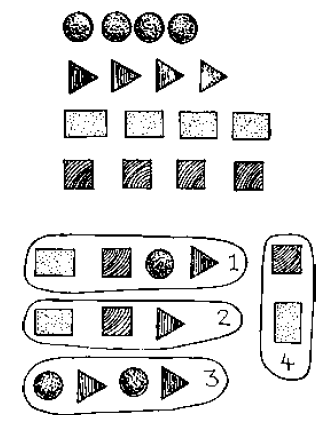
\includegraphics[width=0.4\textwidth]{./img/source/arranging-shapes.png}
\end{center}

\begin{description*}
%\item[Subtopic:]{}
\item[Materials:]{Paper/card, coloured pens/pencils}
%\item[Setup:]{}
\item[Procedure:]{Make four of each of the following shapes: squares (3 cm $\times$ 3 cm) triangle (3 cm sides)
rectangles (3 $\times$ 4 cm) circles (3 cm diameter). Mix the shapes and then sort them according to
a chosen feature.}
%\item[Hazards:]{}
\item[Questions:]{How many different ways can you find of grouping the shapes?}
\item[Observations:]{At least 4 can be found.}
\item[Theory:]{In Biology, classification is used to group things based on shared qualities (i.e. living and non-living things).}
%\item[Applications:]{}
%\item[Notes:]{}
\end{description*}

\vfill
\columnbreak

\subsection{Classification at the Duka} % Source 27

\begin{center}
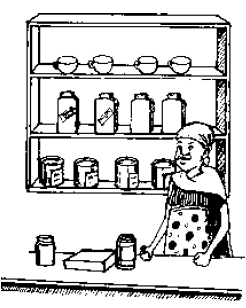
\includegraphics[width=0.38\textwidth]{./img/source/classification-duka.png}
\end{center}

\begin{description*}
%\item[Subtopic:]{}
%\item[Materials:]{}
%\item[Setup:]{}
\item[Procedure:]{Observe how goods at the local shop are arranged on the shelves.}
%\item[Hazards:]{}
\item[Questions:]{Can you find a pattern in the arrangements on the shelves?}
\item[Observations:]{The goods will be arranged firstly in large groups, i.e. foodstuffs, non-food stuffs (medicines,
etc.), and then into smaller groups such as foods in tins, foods in bottles, etc.}
\item[Theory:]{This concept of classification is also used in the study of Biology.}
%\item[Applications:]{}
%\item[Notes:]{}
\end{description*}

\subsection{Find a Missing Person}

\begin{center}
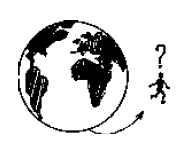
\includegraphics[width=0.35\textwidth]{./img/source/missing-person.png}
\end{center}

\begin{description*}
%\item[Subtopic:]{}
%\item[Materials:]{}
%\item[Setup:]{}
\item[Procedure:]{Imagine that you have been asked to find one particular person on earth.}
%\item[Hazards:]{}
\item[Questions:]{What information would you require?}
\item[Observations:]{Continent, country, region, district, ten cell block, house, name of person.}
\item[Theory:]{This procedure can be compared to the process of classifying organisms, firstly in large
groups (equivalent to a continent), then smaller groups (equivalent to country, region etc).}
%\item[Applications:]{}
%\item[Notes:]{}
\end{description*}

\subsection{Classifying Leaves} % Source 28

\begin{center}
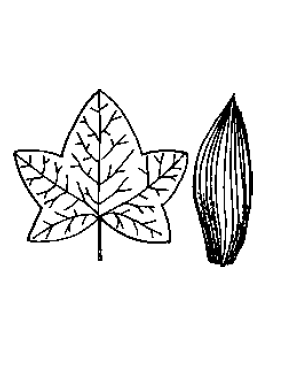
\includegraphics[width=0.4\textwidth]{./img/source/classify-leaves.png}
\end{center}

\begin{description*}
%\item[Subtopic:]{}
%\item[Materials:]{Various leaves}
%\item[Setup:]{}
\item[Procedure:]{Collect leaves from different plants. Make large groups and small groups using as many
different characteristics as possible.}
%\item[Hazards:]{}
\item[Questions:]{How many ways can you find to group the leaves?}
\item[Observations:]{Characteristics like shape, colour, vein pattern, leaf margin etc. can all be used.}
%\item[Theory:]{}
%\item[Applications:]{}
%\item[Notes:]{}
\end{description*}

\subsection{Scavenger Hunt} % Shika 223

%\begin{center}
%\includegraphics[width=0.4\textwidth]{./img/.png}
%\end{center}

\begin{description*}
%\item[Subtopic:]{}
%\item[Materials:]{}
%\item[Setup:]{}
\item[Procedure:]{Find different animals, plants, fungi etc. that are available around the school or at their homes (especially mosses in wet places and fungi near decaying material in the shade). Send students to find different specimen giving hints if necessary. When they return, have them classify what has been found.}
%\item[Hazards:]{}
%\item[Questions:]{}
%\item[Observations:]{}
%\item[Theory:]{}
%\item[Applications:]{}
%\item[Notes:]{}
\end{description*}

\vfill
\columnbreak

\subsection{Display Boards} % VSO 19, Source

\begin{center}
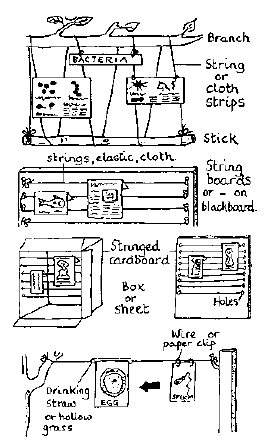
\includegraphics[width=0.49\textwidth]{./img/source/displays.png}
\end{center}

\begin{description*}
%\item[Subtopic:]{}
\item[Materials:]{String, sticks/branches, cardboard boxes, nails, tape}
%\item[Setup:]{}
\item[Procedure:]{Construct display boards as shown to present information about specimen collected. Students can present their displays to the class or as part of a science fair project.}
%\item[Hazards:]{}
%\item[Questions:]{}
%\item[Observations:]{}
%\item[Theory:]{}
%\item[Applications:]{}
\item[Notes:]{See more display ideas in \nameref{cha:displays} (p.~\pageref{cha:displays}).}
\end{description*}

%==================================================================================================%


\end{multicols}

\pagebreak

% Form II
\chapter{Biology Activities for Form II}
%\section{Classification of Living Things}

\begin{multicols}{2}


%\section*{}


\subsection{Investigating Kingdom Fungi} % LASM

%\begin{center}
%\includegraphics[width=0.4\textwidth]{./img/.png}
%\end{center}

\begin{description*}
%\item[Subtopic:]{}
\item[Materials:]{Petri dishes*, water drop microscope*, mushrooms/fungi of various types}
\item[Setup:]{}
\item[Procedure:]{}
\item[Hazards:]{}
\item[Questions:]{}
\item[Observations:]{}
\item[Theory:]{}
\item[Applications:]{}
\item[Notes:]{}
\end{description*}

%==================================================================================================%


\end{multicols}

\pagebreak
\section{Nutrition} \index{Nutrition}

\begin{multicols}{2}


%\section*{Human Nutrition}

%==================================================================================================%

\section*{Properties of Food Substances}


\subsection{Lipids - Fats and Oils} \index{Lipids} % VSO 26

\begin{center}
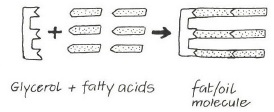
\includegraphics[width=0.45\textwidth]{./img/vso/lipids.jpg}
\end{center}

\begin{description*}
%\item[Subtopic:]{}
\item[Materials:]{Card, scissors}
\item[Setup:]{Cut out the shapes of the glycerol and fatty acid molecules. They can be
combined to form fat (lipid) molecules.}
\item[Procedure:]{Ask students to form fats of different types with the cards. }
%\item[Hazards:]{}
%\item[Questions:]{}
%\item[Observations:]{}
\item[Theory:]{Fats are made up of glycerol and fatty acids. The longer the fatty acid chains
the more solid the lipid. Oils have short chains of fatty acids, fats much
longer ones.}
%\item[Applications:]{}
%\item[Notes:]{}
\end{description*}

\subsection{Solubility of Fats and Oils} % Source 41

\begin{center}
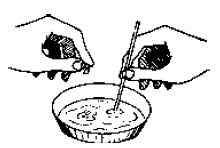
\includegraphics[width=0.4\textwidth]{./img/source/fats-oils-solubility.png}
\end{center}

\begin{description*}
%\item[Subtopic:]{}
\item[Materials:]{Oil, water, petrol, 2 containers}
%\item[Setup:]{}
\item[Procedure:]{Mix fats or oil with water. Then in a separate container mix fats or oils with a small amount
of petrol.}
%\item[Hazards:]{}
\item[Questions:]{Look through the two liquids. Is there a difference?}
\item[Observations:]{Oils and fats dissolve in organic solvents such as petrol or alcohol, but not in water.
However, vigorous shaking with water will produce a cloudy or milky emulsion of suspended
fat droplets.}
%\item[Theory:]{}
%\item[Applications:]{}
%\item[Notes:]{}
\end{description*}

\subsection{Carbohydrates} \index{Carbohydrates} % VSO 26

\begin{center}
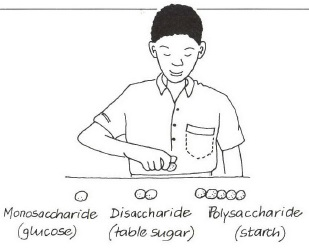
\includegraphics[width=0.4\textwidth]{./img/vso/carbohydrates.jpg}
\end{center}

\begin{description*}
%\item[Subtopic:]{}
\item[Materials:]{Peas, beans or other small identical items}
%\item[Setup:]{}
\item[Procedure:]{Arrange peas or other small objects to make carbohydrate chains of different lengths.}
%\item[Hazards:]{}
%\item[Questions:]{}
%\item[Observations:]{}
\item[Theory:]{Each pea is a monosaccharide,
e.g. glucose. Putting 2 together
makes a disaccharide, e.g. table
sugar, and a long chain of them a
polysaccharide, e.g. starch. 
}
%\item[Applications:]{Toilet
%roll provides another analogy of
%the way identical units combine in
%long chains to make a polysaccharide.}
\item[Notes:]{Not all di- and
polysaccharides consist of
identical units, e.g. sucrose is a
disaccharide of 2 monosaccharides
glucose and fructose.}
\end{description*}

\subsection{Simple Sugar Model} % Source 39

\begin{center}
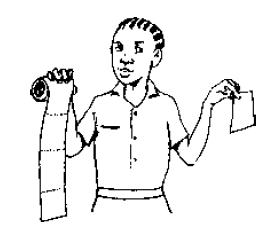
\includegraphics[width=0.4\textwidth]{./img/source/sugar-model.png}
\end{center}

\begin{description*}
%\item[Subtopic:]{}
%\item[Materials:]{}
%\item[Setup:]{}
\item[Procedure:]{To illustrate the long chain structure of polysaccharides use strings of beads, toilet roll or a
chain of pupils. Each long chain is formed by smaller units which represent simple sugars.}
%\item[Hazards:]{}
%\item[Questions:]{}
%\item[Observations:]{}
%\item[Theory:]{}
%\item[Applications:]{}
%\item[Notes:]{}
\end{description*}

\subsection{Protein Molecules} \index{Proteins} % VSO 26

\begin{center}
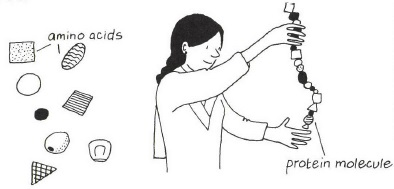
\includegraphics[width=0.49\textwidth]{./img/vso/proteins.jpg}
\end{center}

\begin{description*}
%\item[Subtopic:]{}
\item[Materials:]{Bottle caps, seeds, beans, fruits, paper/card, string, scissors}
%\item[Setup:]{}
\item[Procedure:]{A variety of different shaped and
sized items threaded on a string
show how different types of
amino acids join together to
make a protein molecule.
Students can collect their own
materials and make their own
models, or cut out
shapes from paper or card.}
%\item[Hazards:]{}
%\item[Questions:]{}
%\item[Observations:]{}
%\item[Theory:]{}
%\item[Applications:]{}
%\item[Notes:]{}
\end{description*}

%\subsection{Straightening Hair} % Source 44
%
%\begin{center}
%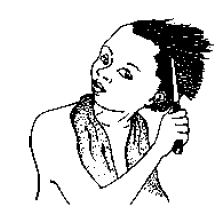
\includegraphics[width=0.35\textwidth]{./img/source/straight-hair.png}
%\end{center}
%
%\begin{description*}
%%\item[Subtopic:]{}
%%\item[Materials:]{}
%%\item[Setup:]{}
%%\item[Procedure:]{}
%%\item[Hazards:]{}
%\item[Observations:]{Some Tanzanian women use a hot comb to straighten their hair.}
%\item[Questions:]{Why can't a cold comb be used?}
%\item[Theory:]{The protein keratin, which is present in hair, has sulphur bonds between protein chains.
%Combing the hair with a hot comb can break these bonds temporarily and thus straighten the
%hair. The bonds soon rejoin and the hair becomes kinky again.}
%%\item[Applications:]{}
%%\item[Notes:]{}
%\end{description*}

%==================================================================================================%

\section*{Food Tests} \index{Food Tests}
%\textbf{*NECTA PRACTICAL*}


\subsection{Test for Lipids} \index{Lipids}% VSO 27, LASM 70

\begin{center}
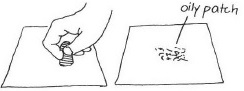
\includegraphics[width=0.45\textwidth]{./img/vso/food-test-lipids.jpg}
\end{center}

\begin{description*}
%\item[Subtopic:]{}
\item[Materials:]{Cooking oil, water, plastic bottles, \nameref{sec:testtubes}, iodine solution, straw}
%\item[Setup:]{}
\item[Procedure:]{Mix about 10 mL of cookingoil and about 100 mL of water in a plastic bottle and shake vigorously. Pour a small amount into a test tube or syringe. Add 3 drops of iodine solution using a straw and shake the tube.}
%\item[Hazards:]{}
%\item[Questions:]{}
\item[Observations:]{You should see the formation of a red ring at the top of the solution, indicating the presence of lipids.}
%\item[Theory:]{}
%\item[Applications:]{}
\item[Notes:]{Alternatively, rub a piece of food onto a piece of paper. Fat is present if there is a translucent stain.}
\end{description*}

\columnbreak

\subsection{Test for Protein} \index{Proteins} % VSO 27

\begin{center}
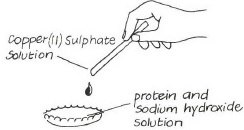
\includegraphics[width=0.45\textwidth]{./img/vso/food-test-protein.jpg}
\end{center}

\begin{description*}
%\item[Subtopic:]{}
\item[Materials:]{Copper (II) sulphate solution, sodium hydroxide solution, food sample (e.g. egg), bottle cap, straw}
%\item[Setup:]{}
\item[Procedure:]{Pour a small amount of egg white into a bottle cap. Add a few drops of sodium hydroxide solution, followed by a small amount of copper (II) sulphate solution.}
%\item[Hazards:]{}
%\item[Questions:]{}
\item[Observations:]{Purple colour indicates the presence of protein in the sample.}
%\item[Theory:]{}
%\item[Applications:]{}
%\item[Notes:]{}
\end{description*}

\subsection{Test for Starch} \index{Starch} % VSO 27

\begin{center}
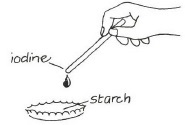
\includegraphics[width=0.4\textwidth]{./img/vso/food-test-starch.jpg}
\end{center}

\begin{description*}
%\item[Subtopic:]{}
\item[Materials:]{Maize flour, iodine solution, bottle cap, water, straw}
\item[Setup:]{Prepare a food sample solution by either saving the remaining water from boiling pasta/potatoes or by mixing 2 teaspoons of maize flour into a litre of water and heating to dissolve.}
\item[Procedure:]{Add a few drops of iodine solution to the sample and observe any changes.}
%\item[Hazards:]{}
%\item[Questions:]{}
\item[Observations:]{A blue-black colour confirms the presence of starch.}
%\item[Theory:]{}
%\item[Applications:]{}
%\item[Notes:]{}
\end{description*}


\columnbreak

\subsection{Test for Reducing Sugars} \index{Reducing sugars} % VSO 27

\begin{center}
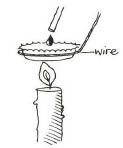
\includegraphics[width=0.25\textwidth]{./img/vso/food-test-reducing.jpg}
\end{center}

\begin{description*}
%\item[Subtopic:]{}
\item[Materials:]{Benedict's solution, \nameref{sec:heatsources}, bottle cap, straw, food sample (e.g. glucose or onions)}
%\item[Setup:]{}
\item[Procedure:]{Dissolve the food in water. Put
some into the bottle top and add
Benedict's solution.
Heat very gently for 1 minute.}
\item[Hazards:]{Safety goggles should be worn. }
%\item[Questions:]{}
\item[Observations:]{If
a precipitate develops - usually
green or brown - this confirms
the presence of sugar.}
%\item[Theory:]{}
%\item[Applications:]{}
%\item[Notes:]{}
\end{description*}

\subsection[Test for Non-Reducing Sugars]{Test for Non-Reducing \hfill \\ Sugars} \index{Non-reducing sugars}

%\begin{center}
%\includegraphics[width=0.4\textwidth]{./img/.png}
%\end{center}

\begin{description*}
%\item[Subtopic:]{}
\item[Materials:]{Benedict's solution, \nameref{sec:heatsources}, sodium hydroxide solution, citric acid, water, food sample (e.g. sugar/sugar cane), }
%\item[Setup:]{}
\item[Procedure:]{Dissolve the food in water. Add a small amount of citric acid and bring to a boil. Allow it to cool and add a small amount of NaOH to the solution and shake. Add a small amount of Benedict's solution and boil again. Allow it to cool and observe changes in appearance.}
%\item[Hazards:]{}
%\item[Questions:]{}
\item[Observations:]{A colour change from green to yellow, then to brick red precipitate indicates the presence of non-reducing sugars.}
%\item[Theory:]{}
%\item[Applications:]{}
%\item[Notes:]{}
\end{description*}

\columnbreak

%==================================================================================================%

\section*{Human Digestive System} \index{Digestive system}


\subsection{Models for Digestion} % VSO 27

\begin{center}
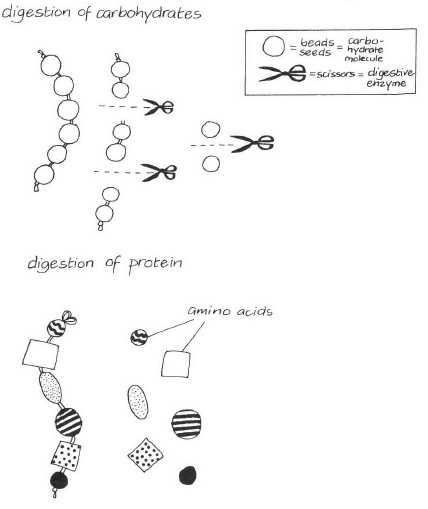
\includegraphics[width=0.49\textwidth]{./img/vso/digestion-models.jpg}
\end{center}

\begin{description*}
%\item[Subtopic:]{}
\item[Materials:]{Beads/seeds/cards, scissors, string}
%\item[Setup:]{}
\item[Procedure:]{String several beads or seeds together to make a chain. Or use toiler paper sheets or paper clips. Cut up or separate the models of food molecules to
demonstrate digestion.}
%\item[Hazards:]{}
\item[Questions:]{What action does cutting with scissors represent?}
\item[Observations:]{The scissor action represents the action of salivary amylase as it breaks down the long
starch chain to simple sugars (maltose).}
\item[Theory:]{Starch is a polysaccharide made up of many identical glucose molecules. 27
Proteins are made up from many different amino acids. During
digestion large molecules are broken down into smaller ones by
enzymes, e.g. starch is broken down into glucose, proteins into the
component amino acids.}
%\item[Applications:]{}
%\item[Notes:]{}
\end{description*}

\vfill
\columnbreak

\subsection{Digestive System Model} % VSO 28

\begin{center}
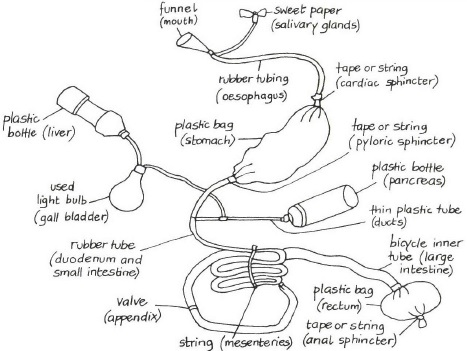
\includegraphics[width=0.49\textwidth]{./img/vso/digestive-sys-model.jpg} \\[6pt]
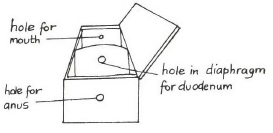
\includegraphics[width=0.4\textwidth]{./img/vso/digestive-sys-model-2.jpg}
\end{center}

\begin{description*}
%\item[Subtopic:]{}
%\item[Materials:]{}
%\item[Setup:]{}
\item[Procedure:]{Have students construct a model of a digestive system using the local materials shown. Colour and label the different sections and mount on a display board. }
%\item[Hazards:]{}
%\item[Questions:]{}
%\item[Observations:]{}
%\item[Theory:]{}
\item[Applications:]{Ask students to place inside a box to demonstrate how the intestine passes through the diaphragm.}
%\item[Notes:]{}
\end{description*}

%\subsection{Types of Teeth} % Source 53
%
%\begin{center}
%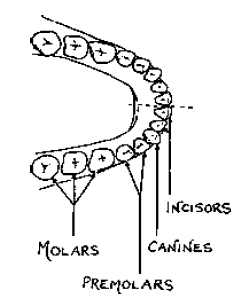
\includegraphics[width=0.3\textwidth]{./img/source/teeth-types.png}
%\end{center}
%
%\begin{description*}
%%\item[Subtopic:]{}
%%\item[Materials:]{}
%%\item[Setup:]{}
%\item[Procedure:]{Look into a friend's mouth. Examine the teeth and differentiate between them. Count the
%number of each type present. Try to identify the function of each.}
%%\item[Hazards:]{}
%\item[Questions:]{How many are there altogether of each type?}
%\item[Observations:]{There are four types of teeth in the buccal cavity and 32 teeth in all.}
%\item[Theory:]{The four different types of teeth perform different functions. The front ones, the incisors,
%are used for cutting. The canines are used for tearing. The premolars may have one or more
%points for cutting, or flat surfaces for grinding. Behind the premolars are the molars with flat
%surfaces for grinding. Molars are not present in young children.}
%%\item[Applications:]{}
%%\item[Notes:]{}
%\end{description*}

\subsection{Invisible Saliva Ink} \index{Saliva} % VSO 29, Source 61

\begin{center}
\includegraphics[width=0.4\textwidth]{./img/source/saliva-ink.png}
\end{center}

\begin{description*}
%\item[Subtopic:]{}
\item[Materials:]{Filter paper/toilet paper, starch solution, iodine solution, matches/cotton swabs}
\item[Setup:]{Prepare a starch solution by adding a teaspoon of maize/cassava flour to half a
cup of water. Bring to a boil, then allow to cool and filter the liquid through a cloth.}
\item[Procedure:]{Soak toilet paper in starch solution. Ask students to use saliva on a matchstick or cotton swab to write their names on the treated paper. Dip the paper in a very dilute iodine solution.}
%\item[Hazards:]{}
%\item[Questions:]{}
%\item[Observations:]{}
\item[Theory:]{The enzymes in the saliva digest the starch where it touches the paper.}
%\item[Applications:]{Enzyme action}
%\item[Notes:]{}
\end{description*}

\subsection{Salts in Saliva} % Source 62

\begin{center}
\includegraphics[width=0.4\textwidth]{./img/source/saliva-salts.png}
\end{center}

\begin{description*}
%\item[Subtopic:]{}
\item[Materials:]{Spoon, candle, dilute HCl}
%\item[Setup:]{}
\item[Procedure:]{Gently heat some saliva on a spoon until it is dry and observe. Then add a small amount of dilute hydrochloric acid.}
%\item[Hazards:]{}
%\item[Questions:]{}
\item[Observations:]{A white residue is left upon heating. Bubbles of carbon dioxide are given off when HCl is added.}
\item[Theory:]{Calcium carbonate is the residue and this reacts with the hydrochloric acid to produce
carbon dioxide.}
%\item[Applications:]{}
%\item[Notes:]{}
\end{description*}

\subsection{Swallowing Upside Down} \index{Peristalsis} % Shika 220, Source 64

\begin{center}
\includegraphics[width=0.35\textwidth]{./img/source/peristalsis.png}
\end{center}

\begin{description*}
%\item[Subtopic:]{}
\item[Materials:]{Drinking water/bread}
%\item[Setup:]{}
\item[Procedure:]{Drink a mouth full of water from a cup and swallow it. Then fill your mouth again, (without
swallowing) and with the help of two friends do a handstand. Then swallow while upside down. Also try with a small piece of bread}
%\item[Hazards:]{}
%\item[Questions:]{}
\item[Observations:]{You are able to swallow while upside down, but not as easily.}
\item[Theory:]{The peristalsis of the
esophagus works against the forces of gravity.}
%\item[Applications:]{}
%\item[Notes:]{}
\end{description*}

\subsection{Peristalsis Model} % VSO 29

\begin{center}
\includegraphics[width=0.4\textwidth]{./img/vso/peristalsis-model.jpg}
\end{center}

\begin{description*}
%\item[Subtopic:]{}
\item[Materials:]{Balloon, rubber band, orange/large seed, large tube}
%\item[Setup:]{}
\item[Procedure:]{A balloon gripped with the hand
pushes air along. You can also
move an object along a tube by
squeezing behind the `food' ball.}
%\item[Hazards:]{}
%\item[Questions:]{}
%\item[Observations:]{}
\item[Theory:]{Food is moved by the contraction
of the muscular walls of the gut.}
%\item[Applications:]{}
%\item[Notes:]{}
\end{description*}

\subsection{Intestine Length} % VSO 28, Source 71

\begin{center}
\includegraphics[width=0.4\textwidth]{./img/vso/intestine-length.jpg}
\end{center}

\begin{description*}
%\item[Subtopic:]{}
\item[Materials:]{Long piece of rope}
%\item[Setup:]{}
\item[Procedure:]{Ask pupils to draw on the ground the shapes of different animals (e.g. rabbit, man, cat/dog,
pig, cow). Try to draw them life size. Then coil string or strips of paper inside the abdominal
cavity area of the animal shape. Approximate lengths of intestines: rabbit 1~m
cat/dog 2~-~5~m, pig 24~m, horse 30~m, cow 50~m.}
%\item[Hazards:]{}
\item[Questions:]{Why do intestine lengths differ an why do herbivores have longer intestines than carnivores?}
%\item[Observations:]{}
\item[Theory:]{Length of intestine corresponds to the type of diet an animal eats. Herbivores have longer
intestines than carnivores in order to break down the plants that they eat.}
%\item[Applications:]{}
%\item[Notes:]{}
\end{description*}

\subsection{Absorption Model} % VSO 29

\begin{center}
\includegraphics[width=0.4\textwidth]{./img/vso/absorption-model.jpg}
\end{center}

\begin{description*}
%\item[Subtopic:]{}
\item[Materials:]{Old shirt sleeve, small objects (e.g. peas), water}
%\item[Setup:]{}
\item[Procedure:]{Place the shirt sleeve over a container to catch the water as it drips
through. Pour the mixture of water and peas down the tube. }
%\item[Hazards:]{}
%\item[Questions:]{}
\item[Observations:]{Water
will leak out, but the peas (undigested food) pass straight down. You
may need to tie off the end of the sleeve to slow the process down.}
%\item[Theory:]{}
%\item[Applications:]{}
\item[Notes:]{Extend the activity by using a semi-permeable plastic bag for the gut.
Pour starch and sugar into the tube and test to see what passed
through.}
\end{description*}

%==================================================================================================%

\section*{Disorders of the Digestive \hfill \\ System}


\subsection{Tooth Decay from Soda} % eggs in soda

\begin{center}
\includegraphics[width=0.35\textwidth]{./img/source/tooth-decay.png}
\end{center}

\begin{description*}
%\item[Subtopic:]{}
\item[Materials:]{Soda, glass, egg or baby tooth}
%\item[Setup:]{}
\item[Procedure:]{Place an egg or old baby tooth into a glass of soda (e.g. coke) and let it sit. Place another egg or tooth in water for comparison. After a while remove the eggs and observe.}
%\item[Hazards:]{}
%\item[Questions:]{}
\item[Observations:]{The soda has reacted with the egg shell or tooth enamel, digesting part of it.}
\item[Theory:]{When a person fails to brush their teeth properly, the food that remains on the teeth is acted
upon by the bacteria producing acids. These acids eat away the enamel and dentine causing
tooth decay.}
%\item[Applications:]{}
\item[Notes:]{Try with dilute HCl in place of soda.}
\end{description*}

%\subsection{Indigestion} % Source 67
%
%\begin{center}
%\includegraphics[width=0.4\textwidth]{./img/source/indigestion.png} % Source 67
%\end{center}
%
%\begin{description*}
%%\item[Subtopic:]{}
%\item[Materials:]{}
%\item[Setup:]{}
%\item[Procedure:]{}
%\item[Hazards:]{}
%\item[Questions:]{}
%\item[Observations:]{}
%\item[Theory:]{}
%\item[Applications:]{}
%\item[Notes:]{}
%\end{description*}

%==================================================================================================%

\section*{Nutrition in Plants} \index{Plants! nutrition}


\subsection{Nutrients from Soil} % Source 76

\begin{center}
\includegraphics[width=0.25\textwidth]{./img/source/nutrients-plants.png}
\end{center}

\begin{description*}
%\item[Subtopic:]{}
\item[Materials:]{2 containers, cardboard, soil, seeds}
%\item[Setup:]{}
\item[Procedure:]{Fill one container with pieces of card board or foam packing cut
into very small pieces. Fill another container with fertile soil and plant a few seeds (peas,
beans or maize) in each one. Water each container throughout the experiment. Examine daily.}
%\item[Hazards:]{}
%\item[Questions:]{}
\item[Observations:]{Seedlings grown in the container without soil are smaller and less healthy with yellow leaves.}
\item[Theory:]{As well as water, carbon dioxide and sunlight, plants require mineral salts in order to grow
and remain healthy. The seedlings grown without soil get only water and so are lacking these
salts.}
%\item[Applications:]{}
%\item[Notes:]{}
\end{description*}

\subsection{Photosynthesis Model} \index{Photosynthesis} % VSO 38

\begin{center}
\includegraphics[width=0.45\textwidth]{./img/vso/photo-model.jpg}
\end{center}

\begin{description*}
%\item[Subtopic:]{}
\item[Materials:]{Card/paper, matches}
%\item[Setup:]{}
\item[Procedure:]{Draw and cut out the symbols shown above. Then arrange them in the correct order to
show the chemical equation for photosynthesis. Use matchsticks for arrows and + symbols.}
%\item[Hazards:]{}
%\item[Questions:]{}
%\item[Observations:]{}
%\item[Theory:]{}
%\item[Applications:]{}
\item[Notes:]{Repeat the above procedure but replace the words in the shapes with the chemical
formulae of the substances involved. These may be written on the reverse side of the first set
of cards.}
\end{description*}

\subsection[Photosynthesis Equation Game]{Photosynthesis Equation \hfill \\ Game} % VSO 39

\begin{center}
\includegraphics[width=0.45\textwidth]{./img/vso/photo-game.jpg}
\end{center}

\begin{description*}
%\item[Subtopic:]{}
\item[Materials:]{Beans, stones, coins, bottle caps, etc.}
%\item[Setup:]{}
\item[Procedure:]{Arrange the items so they
represent the stages of
photosynthesis as shown in the
diagram.}
%\item[Hazards:]{}
%\item[Questions:]{}
%\item[Observations:]{}
%\item[Theory:]{}
%\item[Applications:]{}
%\item[Notes:]{}
\end{description*}

\subsection{Leaf Structure} % LASM 81 / Leaf Sketch Shika 239

\begin{center}
\includegraphics[width=0.4\textwidth]{./img/vso/leaf-structure.jpg}
\end{center}

\begin{description*}
%\item[Subtopic:]{}
\item[Materials:]{White paper, leaves, pencils}
%\item[Setup:]{}
\item[Procedure:]{Cover a leaf with a piece of paper and gently run a pencil over the paper to reveal the outline of the leaf. Repeat for different leaves and identify the different features of the leaves.}
%\item[Hazards:]{}
%\item[Questions:]{}
%\item[Observations:]{}
%\item[Theory:]{}
%\item[Applications:]{}
%\item[Notes:]{}
\end{description*}

\subsection{Plants Need Light} % Source 73

\begin{center}
\includegraphics[width=0.35\textwidth]{./img/source/plants-light.png}
\end{center}

\begin{description*}
%\item[Subtopic:]{}
\item[Materials:]{Stone/brick or black plastic bag}
%\item[Setup:]{}
\item[Procedure:]{Cover an area of grass with a large flat brick/stone or with a black plastic bag so that no
light reaches the plants. Examine the grass after a few days. An alternative is to place a black
plastic bag over green leaves at the end of a branch and seal it by using string, tape or wire.}
%\item[Hazards:]{}
\item[Questions:]{What changes take place in the appearance of the leaves?}
\item[Observations:]{The plants and leaves become pale green or yellow in colour and die eventually.}
\item[Theory:]{Plants need light for photosynthesis. When they lose their green chlorophyll no more light
can be absorbed and they die.}
%\item[Applications:]{}
%\item[Notes:]{}
\end{description*}

\subsection{Extracting Chlorophyll} \index{Chlorophyll} % Source 74

\begin{center}
\includegraphics[width=0.2\textwidth]{./img/source/chlorophyll-extract.png}
\end{center}

\begin{description*}
%\item[Subtopic:]{}
\item[Materials:]{Green leaves, 2 rocks}
%\item[Setup:]{}
\item[Procedure:]{Pick about 5, large soft green leaves. Cut these into small pieces and grind with a stone.
Add a little water to the pulp and pour the mixture into a glass jar or test tune. Leave to settle.}
%\item[Hazards:]{}
%\item[Questions:]{}
\item[Observations:]{The solid material settles out, leaving a green solution.}
\item[Theory:]{The green substance in the water is chlorophyll, which has been released from the cells by
mechanical breaking of the cell membranes by grinding.}
%\item[Applications:]{}
\item[Notes:]{The extraction of chlorophyll works better in alcohol or spirit.}
\end{description*}

\subsection[Chlorophyll and Photosynthesis]{Chlorophyll and \hfill \\ Photosynthesis} % VSO 39, LASM 87

\begin{center}
\includegraphics[width=0.4\textwidth]{./img/variegated-leaf.png}
\end{center}

\begin{description*}
%\item[Subtopic:]{}
\item[Materials:]{Variegated leaf, alcohol, water bath, \nameref{sec:heatsources}, iodine solution}
%\item[Setup:]{}
\item[Procedure:]{Find a leaf which is not all green. Draw the
leaf, carefully identifying the
green areas where chlorophyll is
present. Test the leaf for starch.
(Boil the leaf in alcohol first).
}
%\item[Hazards:]{}
%\item[Questions:]{}
\item[Observations:]{The areas which turn
blue-black during the test are the
areas of the leaf which were
green.}
%\item[Theory:]{}
%\item[Applications:]{}
%\item[Notes:]{}
\end{description*}

\subsection{$\mathrm{\textbf{C}\textbf{O}_\textbf{2}}$ and Photosynthesis} \index{Carbon dioxide! and photosynthesis} % VSO 39, LASM 84

\begin{center}
\includegraphics[width=0.35\textwidth]{./img/vso/co2-photo.jpg}
\end{center}

\begin{description*}
%\item[Subtopic:]{}
\item[Materials:]{Plant, clear plastic bag, rubber band/wire, sodium hydroxide, alcohol, water bath, \nameref{sec:heatsources}, iodine solution}
%\item[Setup:]{}
\item[Procedure:]{Place a clear plastic bag over one
leaf of a plant as shown and leave
it for a day. Test the leaf in the
bag for starch and also test
another on the plant. (Boil leaves
in alcohol before testing for
starch.) }
%\item[Hazards:]{}
%\item[Questions:]{}
\item[Observations:]{The leaf which has been
in the bag will not have starch in
it, i.e. no photosynthesis has
taken place.}
\item[Theory:]{Sodium hydroxide absorbs carbon dioxide.}
%\item[Applications:]{}
%\item[Notes:]{}
\end{description*}

\columnbreak

\subsection[Starch as a Product of Photosynthesis]{Starch as a Product of \hfill \\ Photosynthesis} \index{Starch! and photosynthesis}% Source 75

\begin{center}
\includegraphics[width=0.4\textwidth]{./img/source/photo-starch.png}
\end{center}

\begin{description*}
%\item[Subtopic:]{}
\item[Materials:]{2 potted plants, alcohol, iodine solution, \nameref{sec:heatsources}, straw}
%\item[Setup:]{}
\item[Procedure:]{Take two plants grown in pots and place one in sunlight and the other in a dark cupboard
for 2 days. Pick a leaf from each, but keep them separate. Heat each leaf in some alcohol for about 5 minutes to remove some of the green colour. Take each leaf out and lay it on
a flat surface. Add a few drops of iodine solution.}
%\item[Hazards:]{}
%\item[Questions:]{}
\item[Observations:]{The leaf from the plant grown in the light became a blue-black colour, whereas the one
from the dark was the pale brown colour of iodine.}
\item[Theory:]{When a leaf is exposed to light, photosynthesis occurs producing sugar, which is then
converted to starch for storage. This gives the blue/black colour with iodine. In the dark, no
photosynthesis can take place, so no starch is produced.}
%\item[Applications:]{}
%\item[Notes:]{}
\end{description*}

\vfill
\columnbreak

\subsection[Oxygen as a Product of Photosynthesis]{Oxygen as a Product of \hfill \\ Photosynthesis} \index{Oxygen! and photosynthesis} % Source 74

\begin{center}
\includegraphics[width=0.4\textwidth]{./img/source/photo-gas.png}
\end{center}

\begin{description*}
%\item[Subtopic:]{}
\item[Materials:]{Plastic bottle, large container, water, plants}
%\item[Setup:]{}
\item[Procedure:]{Cut the neck from a plastic bottle, leaving the screw cap in place. Place in a large
container of water making sure the bottle is completely filled with water. Place some aquatic
plants under the bottle and leave for a few days in sunlight.}
%\item[Hazards:]{}
%\item[Questions:]{}
\item[Observations:]{The water level goes down. }
\item[Theory:]{Oxygen produced by photosynthesis forms as bubbles on the
leaves, which rise and collect in the bottle neck.}
%\item[Applications:]{}
%\item[Notes:]{}
\end{description*}

%\subsection{Oxygen as a By-Product of Photosynthesis} % LASM 91
%
%\begin{center}
%\includegraphics[width=0.4\textwidth]{./img/oxygen-photo.png}
%\end{center}
%
%\begin{description*}
%%\item[Subtopic:]{}
%\item[Materials:]{}
%\item[Setup:]{}
%\item[Procedure:]{}
%\item[Hazards:]{}
%\item[Questions:]{}
%\item[Observations:]{}
%\item[Theory:]{}
%\item[Applications:]{}
%\item[Notes:]{}
%\end{description*}

%\subsection{Light and Photosynthesis} % VSO 39
%
%\begin{center}
%\includegraphics[width=0.4\textwidth]{./img/vso/photo-light.jpg}
%\end{center}
%
%\begin{description*}
%%\item[Subtopic:]{}
%\item[Materials:]{2 pot plants, dark cupboard, alcohol, \nameref{sec:heatsources}*, iodine solution}
%%\item[Setup:]{}
%\item[Procedure:]{Take 2 pot plants. Place one in
%sunlight and the other in a dark
%cupboard for 2-3 days. Pick a leaf
%from each plant and remove the
%green colour by heating the
%leaves for about 5 minutes in
%alcohol.
%Test each leaf for starch.}
%\item[Hazards:]{Do not heat the alcohol directly as it is a fire hazard.}
%%\item[Questions:]{}
%\item[Observations:]{The leaf receiving sunlight tests positive for starch, while the one in the cupboard does not.}
%%\item[Theory:]{}
%%\item[Applications:]{}
%%\item[Notes:]{}
%\end{description*}

%\subsection{Test for Starch in Leaves} % LASM 82 Move/combine above?
%
%\begin{center}
%\includegraphics[width=0.4\textwidth]{./img/starch-leaf.png}
%\end{center}
%
%\begin{description*}
%%\item[Subtopic:]{}
%\item[Materials:]{}
%\item[Setup:]{}
%\item[Procedure:]{}
%\item[Hazards:]{}
%\item[Questions:]{}
%\item[Observations:]{}
%\item[Theory:]{}
%\item[Applications:]{}
%\item[Notes:]{}
%\end{description*}

%==================================================================================================%

\section*{Food Preservation} \index{Preservatives}


\subsection{Food Preservatives} % Bill Nye

%\begin{center}
%\includegraphics[width=0.4\textwidth]{./img/.png}
%\end{center}

\begin{description*}
%\item[Subtopic:]{}
\item[Materials:]{4 glasses, bullion cubes, salt, sugar, vinegar, water}
%\item[Setup:]{}
\item[Procedure:]{Heat bullion cubes in water. Pour equal amounts into each of the four glasses. To the first glass, add a spoonful of salt; to another a spoonful of sugar; to another 3 spoonfuls of vinegar; and add nothing to the final glass. Label the glasses accordingly and set in a warm place for 2-3 days.}
%\item[Hazards:]{}
%\item[Questions:]{}
\item[Observations:]{After a couple days, the glass with nothing added is much cloudier than the others.}
\item[Theory:]{The other 3 glasses have been \emph{preserved} using food additives. The glass with no preservative allows more bacteria to grow in the bullion solution.}
\item[Applications:]{Canned foods, food processing}
\item[Notes:]{Conduct an experiment using slices of bread with different preservatives to see which is most effective.}
\end{description*}

%==================================================================================================%


\end{multicols}

\pagebreak
\section{Balance of Nature}

\begin{multicols}{2}


%==================================================================================================%

\section*{The Natural Environment}


\subsection{Disappearing Moths} % VSO 57

%\begin{center}
%\includegraphics[width=0.4\textwidth]{./img/.png}
%\end{center}

\begin{description*}
%\item[Subtopic:]{}
\item[Materials:]{Newspaper, white paper}
%\item[Setup:]{}
\item[Procedure:]{Cut moth shapes from newspaper
and white paper. Place both types
of moth onto newspaper, and
then onto white paper. Note
which moths are easier to see.}
%\item[Hazards:]{}
%\item[Questions:]{}
%\item[Observations:]{}
%\item[Theory:]{}
%\item[Applications:]{}
%\item[Notes:]{}
\end{description*}

\subsection{Camouflage and Protection} % VSO 57

\begin{center}
\includegraphics[width=0.45\textwidth]{./img/vso/camouflage-protection.jpg}
\end{center}

\begin{description*}
%\item[Subtopic:]{}
\item[Materials:]{Long piece of string, 4 pegs, matches, marker pens}
%\item[Setup:]{}
\item[Procedure:]{Mark out an area of grass with
the string and pegs. Colour the
matchsticks with different markers. Make some the same
colour as the grass and others in
very bright colours. Drop the
matches over the area of grass.
}
%\item[Hazards:]{}
\item[Questions:]{Which matches are easiest to
find?}
\item[Observations:]{The green matches blend into their surroundings and hence are safer from predators.}
%\item[Theory:]{}
\item[Applications:]{Discuss with students why
camouflage would be an
advantage to a small maggot and
why it would help a predator too.}
%\item[Notes:]{}
\end{description*}

\subsection{Reactions to Light} % VSO 57

\begin{center}
\includegraphics[width=0.3\textwidth]{./img/vso/reactions-light.jpg}
\end{center}

\begin{description*}
%\item[Subtopic:]{}
\item[Materials:]{2 plates, maggots}
%\item[Setup:]{}
\item[Procedure:]{Paint or cover one half of each of
the plates. Put the plates together
so that half is dark and half in
bright light. Put 10 maggots into
the centre of the bottom plate
and put the `lid' back. Count how
many maggots are in each side
every 10 minutes.}
%\item[Hazards:]{}
%\item[Questions:]{}
\item[Observations:]{The maggots prefer the light.}
%\item[Theory:]{}
%\item[Applications:]{}
%\item[Notes:]{}
\end{description*}

\subsection{Reactions to Humidity}

\begin{center}
\includegraphics[width=0.25\textwidth]{./img/vso/reactions-humidity.jpg}
\end{center}

\begin{description*}
%\item[Subtopic:]{}
\item[Materials:]{Plate, toilet paper, cloth}
%\item[Setup:]{}
\item[Procedure:]{Put dry toilet paper on one side of
a plate and damp paper on the
other. Put a plate on top and
cover it with a cloth so it is dark
underneath. Count how many
maggots are on each side every
10 minutes.}
%\item[Hazards:]{}
%\item[Questions:]{}
\item[Observations:]{The maggots prefer a humid environment.}
%\item[Theory:]{}
\item[Applications:]{Investigate several conditions at
once. For example, put damp
filter paper on one half of the 2
plates. ls the result the same if
both plates are in sunlight? Which
is more important, dampness or
darkness, i.e. do maggots Prefer
light and damp or dark and dry?}
%\item[Notes:]{}
\end{description*}

\subsection{Terrarium} % Shika 227 VSO 123 pic

\begin{center}
\includegraphics[width=0.4\textwidth]{./img/vso/terrarium.jpg}
\end{center}

\begin{description*}
%\item[Subtopic:]{}
\item[Materials:]{Square plastic bottle, sand, soil, rocks, plants, insects, fine gauze}
%\item[Setup:]{}
\item[Procedure:]{Cut a square plastic bottle in half lengthwise. Fill one side with soil, rocks, sticks, moss, insects, etc. and cover and tape with the top half. Poke a few holes for air to enter. Periodically add water by removing and replacing the top lid.}
%\item[Hazards:]{}
%\item[Questions:]{}
%\item[Observations:]{}
%\item[Theory:]{}
%\item[Applications:]{}
%\item[Notes:]{}
\end{description*}

%\subsection{Ant Farm} % Shika 227 PIC!!!
%
%%\begin{center}
%%\includegraphics[width=0.4\textwidth]{./img/.png}
%%\end{center}
%
%\begin{description*}
%%\item[Subtopic:]{}
%\item[Materials:]{}
%\item[Setup:]{}
%\item[Procedure:]{Place a }
%\item[Hazards:]{}
%\item[Questions:]{}
%\item[Observations:]{}
%\item[Theory:]{}
%\item[Applications:]{}
%\item[Notes:]{}
%\end{description*}

\subsection{Aquarium} % Shika 227 

\begin{center}
\includegraphics[width=0.45\textwidth]{./img/vso/aquarium.jpg}
\end{center}

\begin{description*}
%\item[Subtopic:]{}
\item[Materials:]{Cardboard box, clear plastic, tape, scissors, water}
%\item[Setup:]{}
\item[Procedure:]{Cut viewing windows in the sides of a box. Line the box with a large sheet of clear plastic and fill it with water. Attach the plastic firmly around the edges (e.g. with tape).}
%\item[Hazards:]{}
%\item[Questions:]{}
%\item[Observations:]{}
\item[Theory:]{Unlike the terrarium, the aquarium is not sustainable because aquatic organisms often require more oxygen dissolved  in the water than the container can hold. Adding aquatic plants increases the amount of oxygen in the aquarium.}
%\item[Applications:]{}
%\item[Notes:]{}
\end{description*}

%==================================================================================================%

\section*{Interaction of Living and Non-Living Things}


\subsection{Carbon Cycle Cards} % VSO 56

\begin{center}
\includegraphics[width=0.45\textwidth]{./img/vso/carbon-cycle.jpg}
\end{center}

\begin{description*}
%\item[Subtopic:]{}
\item[Materials:]{Cards, paper strips, string}
%\item[Setup:]{}
\item[Procedure:]{Cut out cards showing stages of
the carbon cycle. Link them
together with the paper strips or string to
make a balanced carbon cycle.
Discuss with students the
consequences of increasing one
stage, e.g. burning extra fossil
fuels.}
%\item[Hazards:]{}
%\item[Questions:]{}
%\item[Observations:]{}
%\item[Theory:]{}
%\item[Applications:]{}
\item[Notes:]{Cards can be made for other cycles as well (e.g. water cycle, nitrogen cycle).}
\end{description*}

\subsection{Water Cycle} 

\begin{center}
\includegraphics[width=0.4\textwidth]{./img/source/water-cycle.jpg}
\end{center}

\begin{description*}
%\item[Subtopic:]{}
\item[Materials:]{Cards, paper strips, string}
%\item[Setup:]{}
\item[Procedure:]{Prepare activity cards as with the carbon cycle.}
%\item[Hazards:]{}
%\item[Questions:]{}
%\item[Observations:]{}
%\item[Theory:]{}
%\item[Applications:]{}
\item[Notes:]{}
\end{description*}

\subsection{Nitrogen Cycle}

\begin{center}
\includegraphics[width=0.4\textwidth]{./img/source/nitrogen-cycle.jpg}
\end{center}

\begin{description*}
%\item[Subtopic:]{}
\item[Materials:]{Cards/manila, flip chart}
%\item[Setup:]{}
\item[Procedure:]{Prepare a wall chart of the natural nitrogen
circulation or make cards of the various steps for students to place. }
%\item[Hazards:]{}
%\item[Questions:]{}
%\item[Observations:]{}
\item[Theory:]{When proteins are broken down in
the body, combined nitrogen containing
compounds leave the body with the urine. These
compounds are broken down further by bacteria
to ammonia (NH$_4$) which makes for example
public places of urination smell very badly.
Dead plant and animal tissues are similarly
broken down. The ammonia formed is washed
into the soil, where it is acted upon by different
types of bacteria, eventually converting it into
nitrates and ammonium salts which are needed
by plants to produce proteins. Hence they are
important fertilizers.}
%\item[Applications:]{}
%\item[Notes:]{}
\end{description*}

%==================================================================================================%

\section*{Food Chains and Food Webs}


\subsection{Food Chain Links} % VSO 56

\begin{center}
\includegraphics[width=0.4\textwidth]{./img/vso/food-chain-links.jpg}
\end{center}

\begin{description*}
%\item[Subtopic:]{}
\item[Materials:]{Cardboard, scissors}
%\item[Setup:]{}
\item[Procedure:]{Cut links of the food chain from
stiff cardboard. Label each link
with one part of the food chain.
Put the links together to make a
chain. Make both simple and more complicated chains.}
%\item[Hazards:]{}
\item[Questions:]{What happens if one link in the middle is removed?}
\item[Observations:]{If a middle link is removed, many other links are impacted.}
\item[Theory:]{Removing a single species can have a dramatic impact on the entire ecosystem.}
%\item[Applications:]{}
%\item[Notes:]{}
\end{description*}

\subsection{Food Webs} % VSO 56

\begin{center}
\includegraphics[width=0.4\textwidth]{./img/vso/food-webs.jpg}
\end{center}

\begin{description*}
%\item[Subtopic:]{}
\item[Materials:]{Card, pictures of animals and plants (optional)}
%\item[Setup:]{}
\item[Procedure:]{Either draw pictures of animals
and plants on cards or stick on
pictures cut out from magazines
etc. Make arrows and write on
them the links shown. Arrange
the cards and arrows to make a
food web.}
%\item[Hazards:]{}
%\item[Questions:]{}
%\item[Observations:]{}
%\item[Theory:]{}
%\item[Applications:]{}
%\item[Notes:]{}
\end{description*}

\subsection{Food Web Connections} % Shika 225

%\begin{center}
%\includegraphics[width=0.4\textwidth]{./img/.png}
%\end{center}

\begin{description*}
%\item[Subtopic:]{}
\item[Materials:]{Long rope/string, students}
%\item[Setup:]{}
\item[Procedure:]{Organize students into a circle. Holding the rope tightly, throw the rope to another student. They pull it tight and throw to another (throws do not need to be adjacent). Once the chain is complete, have one student let go of the rope.}
%\item[Hazards:]{}
%\item[Questions:]{}
%\item[Observations:]{}
\item[Theory:]{The food web represents the different interconnected species in an ecosystem - each student is a member of the food chain. If one species becomes extinct (i.e. one student drops the rope), then it impacts the entire food chain. Other species lose connections (i.e. food) and are in threat of extinction themselves.}
%\item[Applications:]{}
\item[Notes:]{Alternatively, select students to sit down, meaning they have gone extinct as a species. This makes it more difficult for the others to remain standing, i.e. adds strain on their existence.}
\end{description*}

%==================================================================================================%


\end{multicols}

\pagebreak
\section{Transport of Materials in Living Things}

\begin{multicols}{2}


\section*{Diffusion}


\subsection{Diffusion in Liquids}

\begin{center}
\includegraphics[width=0.4\textwidth]{./img/vso/diffusion.jpg}
\end{center}

\begin{description*}
%\item[Subtopic:]{}
\item[Materials:]{Plastic water bottle, food colour (liquid or powder)}
%\item[Setup:]{}
\item[Procedure:]{Put a drop or small amount of powdered food colour into the water without shaking and observe what happens.}
%\item[Hazards:]{}
%\item[Questions:]{}
\item[Observations:]{The colour gradually spreads throughout the water.}
\item[Theory:]{This spreading is due to the motion of the particles of food colour. This process is called \emph{diffusion}.}
\item[Applications:]{Organisms utilize diffusion to balance nutrient concentrations in cells and to transfer oxygen into the bloodstream during respiration.}
%\item[Notes:]{}
\end{description*}

\subsection{Smelling Particles}

\begin{description*}
%\item[Subtopic:]{}
\item[Materials:]{Orange or other citrus fruit, box}
%\item[Setup:]{}
\item[Procedure:]{Peel and orange and have students raise their hands when they begin to smell it. Now place a box in front of the orange and repeat the test.}
%\item[Hazards:]{}
%\item[Questions:]{}
\item[Observations:]{Students in the front center of the room should be the first to raise their hands, followed by those near the sides and in the back. When the orange is peeled behind the box it takes longer for the smell to reach the students.}
\item[Theory:]{Tiny particles from the orange peel spread by diffusion to students' noses. The box hinders the motion of the particles and so they reach the students more slowly.}
\item[Applications:]{Air fresheners and other sprays}
%\item[Notes:]{}
\end{description*}

%==================================================================================================%

\section*{Osmosis}




\subsection{Semi-Permeable Membranes}

\begin{center}
\includegraphics[width=0.4\textwidth]{./img/vso/membrane.jpg}
\end{center}

\begin{description*}
%\item[Subtopic:]{}
\item[Materials:]{Glass jar, clear plastic bag, small beads or stones, beans, netting, string/rubber band}
\item[Setup:]{Place the mixture of beads and beans in the jar. Place the net and plastic bag over the top and tie them on securely.}
\item[Procedure:]{Shake the apparatus for a few seconds.}
%\item[Hazards:]{}
%\item[Questions:]{}
\item[Observations:]{Only the small beads pass through the netting. The beans remain in the jar.}
\item[Theory:]{The beads represent small molecules and the net is a semi-permeable membrane. The beans are too large to pass through and hence remain in the jar.}
%\item[Applications:]{Water filters, organism cell membranes}
%\item[Notes:]{}
\end{description*}

\subsection{Osmosis in Dead and Living Tissues}

\begin{center}
\includegraphics[width=0.35\textwidth]{./img/vso/osmosis-dead-living.jpg}
\end{center}

\begin{description*}
%\item[Subtopic:]{}
\item[Materials:]{Potato, knife, 2 dishes of water}
%\item[Setup:]{}
\item[Procedure:]{Cut the potato in half
and boil one piece. When it has
cooled, hollow out the centre of
both pieces and half fill
with the sugar solution.
Peel the lower half of both
pieces and then place each in a dish of water for an hour or so.}
%\item[Hazards:]{}
%\item[Questions:]{}
\item[Observations:]{Water will only enter the unboiled potato.}
\item[Theory:]{Boiling one potato kills its cells and so osmosis does not occur.}
%\item[Applications:]{}
%\item[Notes:]{}
\end{description*}

\columnbreak

\subsection{Vanilla Balloon}

\begin{center}
\includegraphics[width=0.35\textwidth]{./img/vso/osmosis-vanilla.jpg}
\end{center}

\begin{description*}
%\item[Subtopic:]{}
\item[Materials:]{Balloon/plastic bag, vanilla, straw/syringe}
%\item[Setup:]{}
\item[Procedure:]{Place a few drops of vanilla in a deflated balloon. Now blow up the balloon and tie it shut.}
%\item[Hazards:]{}
%\item[Questions:]{}
\item[Observations:]{You can smell the vanilla through the surface of the balloon.}
\item[Theory:]{The balloon acts as a \emph{semi-permeable membrane} which allows some of the vanilla particles to pass through and reach your nose. Other particles remain inside the balloon.}
%\item[Applications:]{}
%\item[Notes:]{}
\end{description*}

\subsection[Osmosis/Active Transport Model]{Osmosis/Active Transport \hfill \\ Model} % Source 79

\begin{center}
\includegraphics[width=0.45\textwidth]{./img/vso/active-transport.jpg}
\end{center}

\begin{description*}
%\item[Subtopic:]{}
\item[Materials:]{Cardboard tray, matchboxes, peas/beans, bottle caps, tape}
%\item[Setup:]{Tape the matchboxes to a tray. The gaps between them should allow small objects to pass (e.g. peas) but prevent
%movement of larger ones (soda bottle caps).}
\item[Setup:]{Tape the matchboxes to a tray, spaced as shown.}
\item[Procedure:]{Place ten soda caps and ten peas in one
side of the tray and twenty peas in the other side. Shake the tray gently. Count the
peas in each side.}
%\item[Hazards:]{}
%\item[Questions:]{}
%\item[Observations:]{}
\item[Theory:]{The
matchboxes represent a selectively
permeable membrane. The spaces
allow small objects through, but
not larger ones. The peas
represent water molecules which
move freely. The bottle caps
represent larger glucose
molecules which need to be
placed in the matchbox drawers
and actively pushed through to
the other side.}
%\item[Applications:]{}
%\item[Notes:]{}
\end{description*}

\columnbreak

\subsection{Potato Osmosis}

\begin{center}
\includegraphics[width=0.49\textwidth]{./img/vso/osmosis-potato-full.jpg}
\end{center}

\begin{description*}
%\item[Subtopic:]{}
\item[Materials:]{Potato, 2 water bottles, salt, water}
\item[Setup:]{Cut two equal size pieces of potato. Fill one bottle with fresh water and the other with a salt water solution.}
\item[Procedure:]{Put one piece of potato in each bottle. Observe over the next few hours.}
%\item[Hazards:]{}
%\item[Questions:]{}
\item[Observations:]{The potato in fresh water swells while the potato in salt water shrivels up.}
\item[Theory:]{Through osmosis, water moves from a region of low concentration to one of high concentration through a semi-permeable membrane (the potato). In fresh water, the potato has the higher salt concentration, so water enters in order to make a balance. In salt water, the concentration of the surrounding water is higher than that of the potato, so water inside the potato moves outside to dilute the salt solution.}
%\item[Applications:]{}
%\item[Notes:]{Try this experiment again with a boiled potato. Do you observe any differences?}
\end{description*}

%\subsection{Osmosis with Eggs} % VSO 25
%
%\begin{center}
%\includegraphics[width=0.4\textwidth]{./img/vso/osmosis-eggs.jpg}
%\end{center}
%
%\begin{description*}
%%\item[Subtopic:]{}
%\item[Materials:]{Empty eggshell, strong salt solution, jar of water}
%%\item[Setup:]{}
%\item[Procedure:]{Remove the hard outer shell at
%one end of the eggshell to
%expose the inner membrane. Half
%fill the egg with salt solution and
%place it in the jar so that the
%water level is above the exposed
%membrane and leave for a couple
%of hours. }
%%\item[Hazards:]{}
%\item[Observations:]{The level of
%the solution inside the egg rises,
%indicating water has crossed the
%membrane, i.e. osmosis has
%occurred.}
%%\item[Questions:]{What happens if you use sugar solution instead of salt? What if you put salt solution in the jar as well as the egg?}
%\item[Theory:]{Water travels from an area of low concentration to an area of high concentration of salts.}
%%\item[Applications:]{}
%%\item[Notes:]{}
%\end{description*}

\subsection{Guard Cells in Osmosis}

\begin{center}
\includegraphics[width=0.49\textwidth]{./img/vso/osmosis-guard-cells.jpg}
\end{center}

\begin{description*}
%\item[Subtopic:]{}
\item[Materials:]{2 long balloons, tape, rubber band}
%\item[Setup:]{}
\item[Procedure:]{Stick the adhesive tape down one
side of each balloon as shown.
When the balloons are both fully
inflated (turgid) the `stoma' is
open. If you let out some of the
air, (the 'guard cells' become
flaccid), the `stoma' closes.}
%\item[Hazards:]{}
%\item[Questions:]{}
%\item[Observations:]{}
%\item[Theory:]{}
%\item[Applications:]{}
%\item[Notes:]{}
\end{description*}

\columnbreak

%==================================================================================================%

\section*{Transport in Mammals}

%==================================================================================================%

\section*{The Mammalian Heart}


\subsection{Heart Pump Action} % VSO 32

\begin{center}
\includegraphics[width=0.49\textwidth]{./img/vso/heart-pump.jpg}
\end{center}

\begin{description*}
%\item[Subtopic:]{}
\item[Materials:]{2 bowls or buckets, rubber/plastic tubing}
%\item[Setup:]{}
\item[Procedure:]{Open and close your hands as
shown while they are in a bucket
or bowl of water. Now hold a
rubber tube as shown. Open and
close the palms again. }
%\item[Hazards:]{}
%\item[Questions:]{}
%\item[Observations:]{}
\item[Theory:]{The opening and closing of the palms represent the relaxation and contraction of the heart
muscles. Blood enters the chambers of the heart when the muscles relax and is forced out
into the vessels as they contract.}
%\item[Applications:]{}
%\item[Notes:]{}
\end{description*}

\subsection{Heart Model} % VSO 32

\begin{center}
\includegraphics[width=0.45\textwidth]{./img/vso/heart-model.jpg}
\end{center}

\begin{description*}
%\item[Subtopic:]{}
\item[Materials:]{Cardboard box, paper}
%\item[Setup:]{}
\item[Procedure:]{Make a model of the heart from a
cardboard box as shown. Thin
paper is used for the valves.}
%\item[Hazards:]{}
%\item[Questions:]{}
%\item[Observations:]{}
\item[Theory:]{The heart is a four-chambered muscular organ. The upper chambers are thin-walled atria,
which receive blood from the veins. The lower two chambers are the thick-walled ventricles
which pump blood into arteries.}
%\item[Applications:]{}
%\item[Notes:]{}
\end{description*}

%==================================================================================================%

\section*{Blood Vessels}

%==================================================================================================%

\subsection{Measuring Pulse} % VSO 32

\begin{center}
\includegraphics[width=0.4\textwidth]{./img/vso/measuring-pulse.jpg}
\end{center}

\begin{description*}
%\item[Subtopic:]{}
%\item[Materials:]{}
%\item[Setup:]{}
\item[Procedure:]{There are various places on the body where the pulse may be taken.
They are (a) under the ear beside the angle of the jaw, (b) at the wrists,
(c) at the temple, (d) behind the collar bone.
Ask students to find the pulse of a partner. If they have difficulty, they
should move their fingers around or apply a little more pressure.}
%\item[Hazards:]{}
%\item[Questions:]{}
%\item[Observations:]{}
%\item[Theory:]{}
\item[Applications:]{Students can compare a partner's pulse rate before and after exercise.}
%\item[Notes:]{}
\end{description*}

\subsection{Simple Stethoscope} % VSO 32

\begin{center}
\includegraphics[width=0.45\textwidth]{./img/vso/stethoscope.jpg}
\end{center}

\begin{description*}
%\item[Subtopic:]{}
\item[Materials:]{Newspaper, plastic bottle, rubber tube}
%\item[Setup:]{}
\item[Procedure:]{Roll a newspaper up into a hollow tube. Place one end of tube against another students rib
cage (in the area of the heart).}
%\item[Hazards:]{}
%\item[Questions:]{}
\item[Observations:]{The heartbeat can be heard.}
%\item[Theory:]{}
\item[Applications:]{A doctor uses a stethoscope to focus the sound from the heart. Another stethoscope idea
could use funnels and plastic tube.}
%\item[Notes:]{}
\end{description*}

%\subsection{Looking at Blood Vessels} % VSO 33
%
%\begin{center}
%\includegraphics[width=0.4\textwidth]{./img/vso/blood-vessels-ex.jpg}
%\end{center}
%
%\begin{description*}
%%\item[Subtopic:]{}
%%\item[Materials:]{}
%%\item[Setup:]{}
%%\item[Procedure:]{}
%%\item[Hazards:]{}
%%\item[Questions:]{}
%\item[Observations:]{The blood capillaries in the corner
%of the eye clearly show capillary
%size. Red meat has so many tiny
%capillaries they give it its colour.}
%%\item[Theory:]{}
%%\item[Applications:]{}
%%\item[Notes:]{}
%\end{description*}

\subsection{Blood Vessel Model} % VSO 33

\begin{center}
\includegraphics[width=0.4\textwidth]{./img/vso/blood-vessels.jpg}
\end{center}

\begin{description*}
%\item[Subtopic:]{}
\item[Materials:]{2 coloured ropes/strings (1 red, 1 blue)}
%\item[Setup:]{}
\item[Procedure:]{Untwist an end of each
rope until each end becomes a
mass of tiny thin strings. If you
twist the thin strings together
they form a mass of fine
capillaries.}
%\item[Hazards:]{}
%\item[Questions:]{}
%\item[Observations:]{}
%\item[Theory:]{}
%\item[Applications:]{}
%\item[Notes:]{}
\end{description*}

%==================================================================================================%

\section*{Blood}

%==================================================================================================%

\subsection{Blood as a Transporter} % VSO 30

\begin{center}
\includegraphics[width=0.49\textwidth]{./img/vso/blood-transport.jpg}
\end{center}

\begin{description*}
%\item[Subtopic:]{}
%\item[Materials:]{}
%\item[Setup:]{}
%\item[Procedure:]{}
%\item[Hazards:]{}
%\item[Observations:]{}
%\item[Theory:]{}
\item[Applications:]{Blood brings substances to the
cells, e.g. food and oxygen, and
removes others (waste and CO$_2$).
A food bar or shop has items
delivered, gives out items and
produces waste. This gives a good
analogy for the blood system.
Students can act out the role of
blood by picking up or putting
down items at different shops
(sites of the body).}
\item[Questions:]{Ask students what they pick up and put down at the following sites: lungs, liver, muscles, kidneys, etc.}
%\item[Notes:]{}
\end{description*}

\columnbreak

\subsection{Red and White Blood Cell Models} % VSO 30

\begin{center}
\includegraphics[width=0.49\textwidth]{./img/vso/red-white-model.jpg}
\end{center}

\begin{description*}
%\item[Subtopic:]{}
\item[Materials:]{Plasticine, clay or wooden rod, card or sponge}
\item[Setup:]{Red blood cells are biconcave discs with no nucleus. You can make
models from Plasticine or circles of wood. White blood cells could be
cut from thin sponge rubber sheet. They contain a nucleus which can
be drawn in on the sponge. Platelets, essential for clotting at open
wounds, can be made from smaller, irregular pieces of sponge, clay etc. }
\item[Procedure:]{Make red and white blood cells
by cutting shapes from cardboard,
paper or plastic.
Add platelets and then put
everything into water. Ask
students what the water
represents.}
%\item[Hazards:]{}
%\item[Questions:]{}
%\item[Observations:]{}
%\item[Theory:]{}
%\item[Applications:]{}
%\item[Notes:]{}
\end{description*}

\subsection{Engulfing Model} % VSO 31

\begin{center}
\includegraphics[width=0.49\textwidth]{./img/vso/engulfing.jpg}
\end{center}

\begin{description*}
%\item[Subtopic:]{}
\item[Materials:]{Clear plastic bag of water or cloth, stone or bean}
%\item[Setup:]{}
\item[Procedure:]{Partly fill a clear plastic bag with
water. Put a stone or bean inside
to represent the nucleus. By
shaping the bag, the action of a
white blood cell engulfing a
foreign body can be
demonstrated. You could use a
cloth, handkerchief or blanket as
a white blood cell. Shape the
cloth to show the pseudopodia
surrounding the foreign body.}
%\item[Hazards:]{}
%\item[Questions:]{}
%\item[Observations:]{}
%\item[Theory:]{}
%\item[Applications:]{}
%\item[Notes:]{}
\end{description*}

\columnbreak

\subsection{Germs and Antibodies} % Source 89

\begin{center}
\includegraphics[width=0.45\textwidth]{./img/source/antibodies-2.png}
\end{center}

\begin{description*}
%\item[Subtopic:]{}
\item[Materials:]{Card, scissors}
%\item[Setup:]{}
\item[Procedure:]{Prepare circles of card with different shapes on their edges as shown in the diagram. The
circles represent the germ and the edge shapes their antigens. Now cut strips of card and
alter one end of each so it matches the edge shapes of the ``germ circles''.}
%\item[Hazards:]{}
%\item[Questions:]{}
%\item[Observations:]{}
\item[Theory:]{The strips of card represent the antibodies produced by the body to combat the antigens of
the germs. The antibodies will be able to act on a specific antigen.}
\item[Applications:]{}
%\item[Notes:]{}
\end{description*}

\subsection{Blood Clotting} % Source 86

\begin{center}
\includegraphics[width=0.3\textwidth]{./img/source/blood-clots.png}
\end{center}

\begin{description*}
%\item[Subtopic:]{}
\item[Materials:]{Red and white beans, container, grass or paper strips}
%\item[Setup:]{}
\item[Procedure:]{Place some red and white beans in a container to represent red and white blood cells.
Move them around by gently shaking. Mix thin strips of grass or paper with the beans and
repeat the shaking action. }
%\item[Hazards:]{}
%\item[Questions:]{}
\item[Observations:]{The beans are packed more securely by the strips.}
\item[Theory:]{The strips
represent the fibrin network }
%\item[Applications:]{}
%\item[Notes:]{}
\end{description*}

\columnbreak

\subsection{Transfusion Checkers} % VSO 31

\begin{center}
\includegraphics[width=0.49\textwidth]{./img/vso/transfusion-checkers.jpg}
\end{center}

\begin{description*}
%\item[Subtopic:]{}
\item[Materials:]{Bottle caps (2 types), card, coloured pens}
%\item[Setup:]{}
\item[Procedure:]{Draw out a base grid as shown. Use 2 types of bottle caps or counters to
show `safe' or `clot' transfusions.}
%\item[Hazards:]{}
\item[Questions:]{Can you place the tops on the right square to show which blood groups are compatible?
Which ones aren't?}
%\item[Observations:]{}
\item[Theory:]{The main red blood cells contain antigens, classified as blood groups A, B or AB. Blood
group O cells do not have antigens. Antibodies in plasma clump blood cells together.}
%\item[Applications:]{}
%\item[Notes:]{}
\end{description*}

\subsection{Transfusion Card Game}

\begin{center}
\includegraphics[width=0.4\textwidth]{./img/vso/transfusion-card.jpg}
\end{center}

\begin{description*}
%\item[Subtopic:]{}
\item[Materials:]{Cards, pen}
\item[Setup:]{Cut out 20 cards and label 5 for each blood group. }
\item[Procedure:]{Shuffle the cards and turn one card face up.
This is the patient's blood group. The next card turned over is the
donor's blood group. If a transfusion is possible, players must call `safe'.
If a transfusion would be dangerous they call `clot'. The first player to
call correctly wins the 2 cards. The player with the most cards wins the game.}
%\item[Hazards:]{}
%\item[Questions:]{}
%\item[Observations:]{}
%\item[Theory:]{}
%\item[Applications:]{}
%\item[Notes:]{}
\end{description*}

\columnbreak

%==================================================================================================%

\section*{Blood Circulation}


\subsection{Circulation Game} % VSO 33
\label{sub:circulation-game}

\begin{center}
\includegraphics[width=0.49\textwidth]{./img/source/circulation-game.png}
%\includegraphics[width=0.49\textwidth]{./img/vso/circulation-game.jpg}
\end{center}

\begin{description*}
%\item[Subtopic:]{}
\item[Materials:]{String or chalk, red and blue flowers/papers, students}
\item[Setup:]{Mark out a model of the circulatory system on the ground using stones, string or chalk. Put
pieces of red flowers or paper in the area marked lungs and pieces of blue flowers or paper in
the area marked body tissues. }
\item[Procedure:]{To begin the game two or three pupils pick up blue petals at
the body tissues and follow the arrows through to the heart and on to the lungs. At the lungs
the pupils drop the blue flowers and pick up the red and return to the body tissues via the
other side of the heart.}
%\item[Hazards:]{}
%\item[Questions:]{}
\item[Observations:]{The pupils represent the flow of blood in the body. They must go through the heart twice
before completing the cycle of double circulation. }
\item[Theory:]{As blood flows it transports substances
such as oxygen (red flowers), carbon dioxide (blue flowers) and food materials. Pupils can
also act as heart valves.}
%\item[Applications:]{}
%\item[Notes:]{}
\end{description*}

%==================================================================================================%

\section*{Transport in Plants}


\subsection{Xylem and Phloem Game} % VSO 41

\begin{center}
\includegraphics[width=0.4\textwidth]{./img/vso/xylem-phloem.jpg}
\end{center}

\begin{description*}
%\item[Subtopic:]{}
\item[Materials:]{Chalk, card/paper, coloured markers}
%\item[Setup:]{}
\item[Procedure:]{Chalk 2 circles on the floor or
table. Cut out 20 discs from card
or paper. Colour 10 to represent
xylem vessels and 10 to represent
phloem tubes. Use the discs
to show the arrangement of
vascular tissue in a root and a
dicotyledon stem.}
%\item[Hazards:]{}
\item[Questions:]{What are the differences in arrangement between stem and root?}
%\item[Observations:]{}
\item[Theory:]{Vascular tissue forms a ring of bundles in the stem but a central column in the root.}
%\item[Applications:]{}
%\item[Notes:]{}
\end{description*}

\subsection{Root Hairs} % Source 98

\begin{center}
\includegraphics[width=0.3\textwidth]{./img/source/root-hairs.png}
\end{center}

\begin{description*}
%\item[Subtopic:]{}
\item[Materials:]{Pea/bean seeds, damp cloth}
%\item[Setup:]{}
\item[Procedure:]{Germinate some peas or bean seeds on a damp cloth or newspaper. Leave them until the
young root emerges. Observe the root tip using a hand lens if necessary.}
%\item[Hazards:]{}
%\item[Questions:]{}
\item[Observations:]{A fine covering of thin hair-like structures can be seen, just behind the root tip.}
\item[Theory:]{A root develops hairs just behind the growing tip. As the root gets older and larger the root
hairs are lost. Root hairs increase the surface area of the root for absorption of water and
mineral salts.}
%\item[Applications:]{}
%\item[Notes:]{}
\end{description*}

%\subsection{Capillarity}
%\begin{description*}
%%\item[Subtopic:]{}
%\item[Materials:]{Clear thin plastic straws with different diameters, shallow container (bottom of a water bottle/jar cap), various liquids, e.g. water, spirit and cooking oil}
%%\item[Setup:]{}
%\item[Procedure:]{Place one end of a straw into a container of water 1 cm deep so that the end is submerged but not touching the bottom. Mark the change in water level in the straw after about a minute. Repeat for different liquids and different size straws.}
%%\item[Hazards:]{}
%\item[Questions:]{Which liquid rises the farthest up the straw? Do liquids rise faster in wide or thin straws?}
%\item[Observations:]{The spirit rises to the greatest height while water rises the least. Liquids rise faster in thin straws compared to thick ones.}
%\item[Theory:]{Capillary rise results from adhesion, allowing the liquid to climb along the surface of the tube, as well as cohesion, which pulls the remainder of the liquid up. In a thin container, a larger proportion of liquid is attached to the side of the tube and a smaller proportion is being held by surface tension, so the adhesive force is strong enough to pull all the liquid up the tube.}
%%\item[Applications:]{}
%%\item[Notes:]{}
%\end{description*}

\columnbreak

\subsection{Capillary Rise}

\begin{center}
\includegraphics[width=0.4\textwidth]{./img/source/capillary-glass.jpg}
\end{center}

\begin{description*}
%\item[Subtopic:]{}
\item[Materials:]{2 glass sheets, match, rubber bands, water, food colour (optional)}
%\item[Setup:]{}
\item[Procedure:]{With the help of a rubber band and a matchstick, arrange two clean glass sheets as shown
in the diagram. Place the arrangement in a plate containing some water.}
%\item[Hazards:]{}
%\item[Questions:]{}
\item[Observations:]{Water rises to different heights along and between the glass sheets. }
\item[Theory:]{This is capillary
action. Capillary rise results from adhesion, allowing the liquid to climb along the surface of the glass, as well as cohesion, which pulls the remainder of the liquid up. Water rises more where the glass sheets are closer together.}
%\item[Applications:]{}
%\item[Notes:]{}
\end{description*}

%\subsection{Capillary Rise}
%
%\begin{center}
%\includegraphics[width=0.4\textwidth]{./img/source/capillary-rise.jpg}
%\end{center}
%
%\begin{description*}
%%\item[Subtopic:]{}
%\item[Materials:]{Straws/chalk of different sizes, bottle, food colour, various liquids, e.g. water, spirit, kerosene, cooking oil}
%\item[Setup:]{Cut the bottom of a bottle to make a small dish.}
%\item[Procedure:]{Place one end of a straw/chalk into a dish of water 1 cm deep. Mark the change in level of the food colour after about a minute. Repeat for different liquids and different size straws.}
%%\item[Hazards:]{}
%\item[Questions:]{Which liquid rises the farthest up the straw? Do liquids rise faster in wide or thin straws?}
%\item[Observations:]{The spirit rises to the greatest height while water rises the least. Liquids rise faster in thin straws compared to thick ones.}
%\item[Theory:]{%Capillary rise results from adhesion, allowing the liquid to climb along the surface of the tube, as well as cohesion, which pulls the remainder of the liquid up. 
%In a thin container, a larger proportion of liquid is attached to the side of the tube and a smaller proportion is being held by surface tension, so the adhesive force is strong enough to pull more liquid up the tube.}
%%\item[Applications:]{}
%%\item[Notes:]{}
%\end{description*}

%\subsection{Moving Matches}
%
%%\begin{center}
%%\includegraphics[width=0.4\textwidth]{./img/.png}
%%\end{center}
%
%\begin{description*}
%%\item[Subtopic:]{}
%\item[Materials:]{Matches, water, straw, plastic lid}
%%\item[Setup:]{}
%\item[Procedure:]{Break several matches near the middle, but not so that they come apart. They should make acute angles. Place them on the plastic lid and place a few drops of water on the broken joints of the matches using the straw.}
%%\item[Hazards:]{}
%%\item[Questions:]{}
%\item[Observations:]{The matches close and return to their original straight shape.}
%\item[Theory:]{Water gets absorbed in the wooden matchstick and causes it to expand.}
%\item[Applications:]{This is why it is difficult to open a wooden door after it rains. The water rises up the wood causing it to expand into its frame.}
%%\item[Notes:]{}
%\end{description*}
%
%\columnbreak

%\subsection{Measuring Capillary Rise}
%
%\begin{center}
%\includegraphics[width=0.4\textwidth]{./img/source/capillary-rise-meas.jpg}
%\end{center}
%
%\begin{description*}
%%\item[Subtopic:]{}
%\item[Materials:]{Paper, chalk, small dish/lid, water, food colour}
%\item[Setup:]{Cut off the bottom of a plastic bottle to make a water dish.}
%\item[Procedure:]{Place a strip of paper and a piece of chalk in a dish containing water. Leave the objects for some time and measure the rise in colour of each using a ruler.}
%%\item[Hazards:]{}
%%\item[Questions:]{}
%\item[Observations:]{The water rises faster in the chalk than in the paper.}
%\item[Theory:]{Chalk has smaller capillaries than paper, which allows water to rise faster.}
%%\item[Applications:]{}
%%\item[Notes:]{}
%\end{description*}

\subsection{Automatic Irrigation}

\begin{center}
\includegraphics[width=0.3\textwidth]{./img/source/irrigation.png}
\end{center}

\begin{description*}
%\item[Subtopic:]{}
%\item[Materials:]{}
%\item[Setup:]{}
%\item[Procedure:]{}
%\item[Hazards:]{}
%\item[Questions:]{}
%\item[Observations:]{}
%\item[Theory:]{}
\item[Applications:]{Capillary action can be used to provide automatic irrigation for plants. Students can perform irrigation by dipping a porous material such as paper or cotton cloth in water.}
%\item[Notes:]{}
\end{description*}

\subsection{Water Movement in Plants} % VSO 41

\begin{center}
\includegraphics[width=0.4\textwidth]{./img/vso/water-movement.jpg}
\end{center}

\begin{description*}
%\item[Subtopic:]{}
\item[Materials:]{Various plant stems, food colour/ink (not black), water, knife}
%\item[Setup:]{}
\item[Procedure:]{Place a variety of different types of plants in coloured ink or dye and
leave them for a few hours. Slice off sections of the stem with a sharp
knife and examine them under a hand lens. }
%\item[Hazards:]{}
%\item[Questions:]{}
\item[Observations:]{The colour is located in the
xylem vessels which shows water is transported in the xylem. Some very young plants, such as
Balsam, are so transparent that
you can see the colour move up
the stem.}
%\item[Theory:]{}
%\item[Applications:]{}
%\item[Notes:]{}
\end{description*}

\subsection{Transpiration} % VSO 40

\begin{center}
\includegraphics[width=0.4\textwidth]{./img/vso/transpiration.jpg}
\end{center}

\begin{description*}
%\item[Subtopic:]{}
\item[Materials:]{Potted plant, 2 small plastic bags, string, grease/Vaseline}
%\item[Setup:]{}
\item[Procedure:]{Place a polythene bag over the leaf of a living plant. Secure the bag to the stem with a
thread. Repeat the experiment with a greased leaf of the same size.}
%\item[Hazards:]{}
%\item[Questions:]{}
\item[Observations:]{Water droplets appear on the inside of the bag placed over the ungreased leaf. Very little
or no water collects in the other bag.}
\item[Theory:]{Water, which is absorbed from the soil by the plant, is lost through the pores (stomata) of the leaf. This is transpiration. There is no water loss from the greased leaf because the
grease blocks the pores.}
%\item[Applications:]{}
%\item[Notes:]{}
\end{description*}

%==================================================================================================%


\end{multicols}

\pagebreak
\section{Gaseous Exchange and Respiration} 

\begin{multicols}{2}


\section*{Gas Exchange in Mammals} \index{Gas exchange! in mammals} \index{Mammals! gas exchange in}


\subsection{Breathing Model} % VSO 34

\begin{center}
\includegraphics[width=0.49\textwidth]{./img/vso/breathing-model.jpg}
\end{center}

\begin{description*}
%\item[Subtopic:]{}
\item[Materials:]{Plastic bottle, balloons, plastic bag, string/rubber band, straw}
%\item[Setup:]{}
\item[Procedure:]{Cut the bottom off a plastic
bottle. Attach a balloon over the
bottle mouth so it hangs inside.
Fix a piece of plastic bag over the
cut base end using string or a rubber band. (Optional: Fix a straw through the bottle top and attach 1 or 2 balloons to the end inside the bottle.)}
%\item[Hazards:]{}
%\item[Questions:]{}
\item[Observations:]{Pulling the plastic bag down causes the balloon to inflate; pushing it up causes the balloon the deflate.}
\item[Theory:]{The balloon(s) represents the lung(s), the plastic bag the diaphragm, the bottle the thoracic cavity (and the straw the esophagus). Pulling the plastic sheet down causes an expansion of the cavity bringing about inspiration and causing the balloon to inflate. Pushing the sheet up reduces the volume of the cavity, causing expiration and the balloon to deflate.}
%\item[Applications:]{}
\item[Notes:]{Tell students that this model does not show the expansion and contraction of the rib cage with breathing.}
\end{description*}

\subsection{Lung Capacity} \index{Lung capacity}

\begin{center}
\includegraphics[width=0.4\textwidth]{./img/vso/lung-capacity.jpg}
\end{center}

\begin{description*}
%\item[Subtopic:]{}
\item[Materials:]{Large plastic bag, bucket, water, basin}
%\item[Setup:]{}
\item[Procedure:]{Fill the bucket to the brim with water and stand it in the basin. Blow
into an empty plastic bag or balloon. Submerge the bag in the bucket. Collect the
overflowing water and measure the volume. Do this for regular breaths, deep breaths and breaths after holding for 10 seconds.}
%\item[Hazards:]{}
%\item[Questions:]{}
\item[Observations:]{A regular breath may be around 0.5 L, while a full breath can exceed 3 L.}
%\item[Theory:]{}
%\item[Applications:]{}
%\item[Notes:]{}
\end{description*}

%\subsection{Lung Capacity}
%
%\begin{center}
%\includegraphics[width=0.4\textwidth]{./img/source/lung-capacity.png}
%\end{center}
%
%\begin{description*}
%%\item[Subtopic:]{}
%\item[Materials:]{1.5 L bottle, basin, water, plastic tubes/straws, soap, marker, ruler}
%\item[Setup:]{Make a scale on the bottle using a marker and ruler (e.g. 100 mL increments). Prepare a soap solution for washing the tubes/straws.}
%\item[Procedure:]{Fill a basin with water. Fill a 1.5 L bottle with water and invert it in the basin so that the mouth of the bottle is underneath the water. Place one end of the tube/straw inside the bottle under water. Blow into the tube. Repeat for normal breaths, deep breaths and breaths after holding your breath for 10 seconds.}
%\item[Hazards:]{Wash the tube/straw after each student's use.}
%%\item[Questions:]{}
%\item[Observations:]{The exhaled air displaces water in the bottle. Note the starting and finishing points on the scale to find the \emph{difference}, which is equal to the volume of air exhaled.}
%\item[Theory:]{When we breath in air, our bodies use the oxygen and produce carbon dioxide in a process called \emph{respiration}. Oxygen is transported in our blood throughout our bodies. When we hold our breath, oxygen is not circulated throughout our bodies and we begin to feel lightheaded.}
%%\item[Applications:]{}
%%\item[Notes:]{}
%\end{description*}

\subsection{Gas Exchange Game} % VSO 35

\begin{center}
\includegraphics[width=0.45\textwidth]{./img/vso/gas-exchange-students.jpg}
\end{center}

\begin{description*}
%\item[Subtopic:]{}
\item[Materials:]{Cards, table}
%\item[Setup:]{}
\item[Procedure:]{The table represents the alveolus.
Students wear either an `R' or `P'
card and so act as red blood cells
(R) or plasma (P). When going
round the table the `R' students
pick up cards with `O'(oxygen)
on them. The `P' students put down the
`CO$_2$' (carbon dioxide) cards.}
%\item[Hazards:]{}
%\item[Questions:]{}
%\item[Observations:]{}
%\item[Theory:]{}
\item[Applications:]{Link this activity with \nameref{sub:circulation-game} (p.~\pageref{sub:circulation-game}).}
%\item[Notes:]{}
\end{description*}

\columnbreak

\subsection{Gas Exchange Board Game}

\begin{center}
\includegraphics[width=0.5\textwidth]{./img/vso/gas-exchange-game.jpg}
\end{center}

\begin{description*}
%\item[Subtopic:]{}
\item[Materials:]{Large sheet of paper, bottle caps, seeds, stones}
%\item[Setup:]{}
\item[Procedure:]{Draw the capillary and alveolus as
shown. Students arrange the
stones (oxygen), seeds (carbon
dioxide) and bottle caps (red
blood cells) on the drawing. Colour the bottle caps red inside and blue outside.}
%\item[Hazards:]{}
%\item[Questions:]{}
%\item[Observations:]{}
\item[Theory:]{As the caps (red blood cells) enter the capillary, most are turned to blue to show they contain no stone (oxygen). Stones are placed inside the alveolus which get moved into the capillary and transported away inside red upturned bottle caps (oxygenated red blood cells). The seeds (carbon dioxide) are moved from the capillary plasma area into the alveolus.}
%\item[Applications:]{}
%\item[Notes:]{}
\end{description*}

%==================================================================================================%

\section*{Gas Exchange in Plants} \index{Gas exchange! in plants} \index{Plants! gas exchange in}


\subsection{Germinating Seeds} \index{Germination} % Source 113

\begin{center}
%\includegraphics[width=0.4\textwidth]{./img/source/germinating-seeds.png}
\includegraphics[width=0.3\textwidth]{./img/vso/respiration-co2.jpg}
\end{center}

\begin{description*}
%\item[Subtopic:]{}
\item[Materials:]{Glass jar, limewater, plastic bag, peas}
%\item[Setup:]{}
\item[Procedure:]{Put some lime water into a wide-mouthed glass jar and hang a perforated plastic bag,
containing soaked and germinating peas. Make sure that the peas are separated from the
liquid. Seal the jar well and leave it to stand for a few hours.}
%\item[Hazards:]{}
%\item[Questions:]{}
\item[Observations:]{The limewater becomes cloudy.}
\item[Theory:]{The germinating peas respire, giving out carbon dioxide.}
%\item[Applications:]{}
%\item[Notes:]{}
\end{description*}

\columnbreak

%==================================================================================================%

\section*{Respiration} \index{Respiration}


\subsection{Respiration Cards} % VSO 36

\begin{center}
\includegraphics[width=0.49\textwidth]{./img/vso/respiration-cards.jpg}
\end{center}

\begin{description*}
%\item[Subtopic:]{}
\item[Materials:]{Cards}
%\item[Setup:]{}
\item[Procedure:]{Cut out cards to represent the substances involved in respiration. Label
some cards with a `+' or an arrow. Mix up the cards and ask students to
arrange them correctly as shown.}
%\item[Hazards:]{}
%\item[Questions:]{}
%\item[Observations:]{}
%\item[Theory:]{}
%\item[Applications:]{}
%\item[Notes:]{}
\end{description*}

\subsection{Respiration Plates}

\begin{center}
\includegraphics[width=0.49\textwidth]{./img/vso/respiration-plates.jpg}
\end{center}

\begin{description*}
%\item[Subtopic:]{}
\item[Materials:]{Various seeds, bottle caps, coins, etc., plates, card}
%\item[Setup:]{}
\item[Procedure:]{Choose 3 different types of seed, coin or bottle cap to represent carbon,
hydrogen and oxygen. Arrange 4 plates or boxes on a table as shown.
Ask students to place the correct number of seeds etc. on the plates.
When the seeds are placed correctly the card carrying the `E' for energy
is added.}
%\item[Hazards:]{}
%\item[Questions:]{}
%\item[Observations:]{}
%\item[Theory:]{}
\item[Applications:]{Demonstrate that the reverse equation is the process of
photosynthesis.}
%\item[Notes:]{}
\end{description*}

\subsection{Exhaling \textbf{CO}$_\textbf{2}$} \index{Carbon dioxide! in respiration} % VSO 34 Shika 107

\begin{center}
\includegraphics[width=0.4\textwidth]{./img/vso/exhale-co2.jpg}
\end{center}

\begin{description*}
%\item[Subtopic:]{}
\item[Materials:]{Straw or pen tube, limewater}
%\item[Setup:]{}
\item[Procedure:]{Breathe out through a straw or the barrel of a ball point pen into filtered limewater.}
%\item[Hazards:]{}
%\item[Questions:]{}
\item[Observations:]{The limewater goes cloudy then later clear.}
\item[Theory:]{The exhaled carbon dioxide reacts with the calcium hydroxide solution (lime water) making a precipitation, which later dissolves by more carbon dioxide to soluble calcium hydrogen
carbonate.}
%\item[Applications:]{}
%\item[Notes:]{}
\end{description*}

\subsection{Yeast Balloons} % Shika 221 PIC!!!

\begin{center}
\includegraphics[width=0.3\textwidth]{./img/vso/yeast-balloon.jpg}
\end{center}

\begin{description*}
%\item[Subtopic:]{}
\item[Materials:]{Bottle, balloon, warm water, sugar, yeast}
%\item[Setup:]{}
\item[Procedure:]{Fill a bottle partly with a warm water/sugar solution. Add a small amount of yeast into a balloon. Stretch the mouth of the balloon over the bottle, then lift the balloon to empty its contents into the bottle.}
%\item[Hazards:]{}
%\item[Questions:]{}
\item[Observations:]{After a few hours, the balloon inflates.}
\item[Theory:]{Yeast is a an organism that eats sugar and breaks it down into alcohols and carbon dioxide. The carbon dioxide gets collected in the balloon.}
\item[Applications:]{This process is the basis for making beers, wines and other alcoholic beverages.}
%\item[Notes:]{}
\end{description*}

\columnbreak

\subsection{Fermenting Fruits} \index{Fermentation} % Source 114

\begin{center}
\includegraphics[width=0.4\textwidth]{./img/source/fermenting-fruits.png}
\end{center}

\begin{description*}
%\item[Subtopic:]{}
\item[Materials:]{Fruit pulp (e.g. pawpaw), sugar, water, container}
%\item[Setup:]{}
\item[Procedure:]{Prepare a pulp of paw paw. Put the pulp into a glass. Let it stand for some time in a warm
place.}
%\item[Hazards:]{}
%\item[Questions:]{}
\item[Observations:]{Gas bubbles are formed in the pulp}
\item[Theory:]{The pulp is fermented because the sugar contained in it is acted on by wild yeast, which
grows on the skin of the fruit. Yeasts are also found in air.}
\item[Applications:]{Making local brews (e.g. pombe)}
%\item[Notes:]{}
\end{description*}

\subsection{Fermenting Sugar}

\begin{center}
\includegraphics[width=0.4\textwidth]{./img/vso/fermentation.jpg}
\end{center}

\begin{description*}
%\item[Subtopic:]{}
\item[Materials:]{Yeast, sugar, bottle, tube, water, limewater (optional)}
\item[Setup:]{Poke a hole through a bottle cap using a hot nail and insert a plastic tube. Seal with super glue.}
\item[Procedure:]{Place some yeast in a solution of sugar and water. Cap the bottle and feed the free end of the tube into a dish containing limewater or another bottle full of liquid.}
%\item[Hazards:]{}
%\item[Questions:]{}
\item[Observations:]{The limewater turns cloudy or air bubbles can be seen escaping from the liquid in the dish.}
\item[Theory:]{The yeast organisms break down the sugar and produce carbon dioxide gas through respiration.}
%\item[Applications:]{}
%\item[Notes:]{}
\end{description*}


\end{multicols}

\pagebreak

% Form III
\chapter{Biology Activities for Form III}
%\section{Classification of Living Things}

\begin{multicols}{2}


\section*{}


\subsection{}

\begin{center}
\includegraphics[width=0.4\textwidth]{./img/.png}
\end{center}

\begin{description*}
%\item[Subtopic:]{}
\item[Materials:]{}
\item[Setup:]{}
\item[Procedure:]{}
\item[Hazards:]{}
\item[Questions:]{}
\item[Observations:]{}
\item[Theory:]{}
\item[Applications:]{}
\item[Notes:]{}
\end{description*}

%==================================================================================================%


\end{multicols}

\pagebreak
\section{Movement}

\begin{multicols}{2}


\section*{Human Skeleton}


\subsection{Paper Skeleton} % VSO 44

\begin{center}
\includegraphics[width=0.4\textwidth]{./img/source/skeleton-full.png}
\end{center}
Construct a paper skeleton as shown using 8 sheets of A4 paper. Pin or staple the skeleton together or mount it on a hanging mat.
%\begin{description*}
%%\item[Subtopic:]{}
%\item[Materials:]{8 sheets of paper}
%%\item[Setup:]{}
%\item[Procedure:]{To make the paper skeleton
%shown here you will need 8 pages
%of A4 paper or pages from a large
%writing book used by students.
%Fold and cut out the shapes as
%illustrated for each part of the
%body. The final result should look
%like the one shown.}
%%\item[Hazards:]{}
%%\item[Questions:]{}
%%\item[Observations:]{}
%%\item[Theory:]{}
%%\item[Applications:]{}
%\item[Notes:]{Pin or staple the skeleton together or mount it on a hanging mat.}
%\end{description*}

\subsubsection{Skull and Pelvis}

\begin{center}
\includegraphics[width=0.49\textwidth]{./img/source/skeleton-skull-pelvis.png}
\end{center}

\begin{description*}
%\item[Subtopic:]{}
%\item[Materials:]{}
%\item[Setup:]{}
\item[Skull:]{Cut around the dotted line after
drawing. The teeth and mouth
can be cut without removing any
paper.}
\item[Pelvis:]{Draw half of the pelvis and cut out the basic shape when the paper is
folded}
%\item[Questions:]{}
%\item[Observations:]{}
%\item[Theory:]{}
%\item[Applications:]{}
%\item[Notes:]{}
\end{description*}

\columnbreak

\subsubsection{Limbs}

\begin{center}
\includegraphics[width=0.49\textwidth]{./img/source/skeleton-limbs.png}
\end{center}
The lower limbs are cut out from one piece of paper. The upper limbs
all fit onto another piece.
%\begin{description*}
%%\item[Subtopic:]{}
%%\item[Materials:]{}
%%\item[Setup:]{}
%%\item[Procedure:]{}
%%\item[Hazards:]{}
%%\item[Questions:]{}
%%\item[Observations:]{}
%%\item[Theory:]{}
%%\item[Applications:]{}
%%\item[Notes:]{}
%\end{description*}

\subsubsection{Rib Cage}

\begin{center}
\includegraphics[width=0.49\textwidth]{./img/source/skeleton-ribs.png}
\end{center}
Fold the paper twice and then cut along alternate lines. Use a ruler to
measure accurately if you want to have the exact number of ribs. You
can cut the ribs out of the paper lengthwise instead.
%\begin{description*}
%%\item[Subtopic:]{}
%%\item[Materials:]{}
%%\item[Setup:]{}
%%\item[Procedure:]{}
%%\item[Hazards:]{}
%%\item[Questions:]{}
%%\item[Observations:]{}
%%\item[Theory:]{}
%%\item[Applications:]{}
%%\item[Notes:]{}
%\end{description*}

\subsubsection{Backbone}

\begin{center}
\includegraphics[width=0.2\textwidth]{./img/source/skeleton-backbone.png}
\end{center}
Cut out 2 strips for the backbone
to give extra strength. 
%Stick one
piece to each side of the skeleton.
%\begin{description*}
%%\item[Subtopic:]{}
%%\item[Materials:]{}
%%\item[Setup:]{}
%%\item[Procedure:]{}
%%\item[Hazards:]{}
%%\item[Questions:]{}
%%\item[Observations:]{}
%%\item[Theory:]{}
%%\item[Applications:]{}
%%\item[Notes:]{}
%\end{description*}

\subsubsection{Hands and Feet}

\begin{center}
\includegraphics[width=0.49\textwidth]{./img/source/skeleton-hands-feet.png}
\end{center}
Fold the paper in half and draw around a hand. Use
another piece of paper for the feet.
%\begin{description*}
%%\item[Subtopic:]{}
%%\item[Materials:]{}
%%\item[Setup:]{}
%%\item[Procedure:]{}
%%\item[Hazards:]{}
%%\item[Questions:]{}
%%\item[Observations:]{}
%%\item[Theory:]{}
%%\item[Applications:]{}
%%\item[Notes:]{}
%\end{description*}

\subsection{Robotic Hand}

\begin{center}
\includegraphics[width=0.49\textwidth]{./img/robotic-hand-use.jpg}
\end{center}

\begin{description*}
%\item[Subtopic:]{}
\item[Materials:]{Rubber bands, straws, cardboard, string, masking tape, scissors}
%\item[Setup:]{}
%\item[Procedure:]{}
%\item[Hazards:]{}
%\item[Questions:]{}
%\item[Observations:]{}
%\item[Theory:]{}
%\item[Applications:]{}
%\item[Notes:]{}
\end{description*}

\subsubsection{Hand Structure}

\begin{center}
\includegraphics[width=0.49\textwidth]{./img/robotic-hand-1.jpg}
\end{center}

\begin{description*}
%\item[Subtopic:]{}
%\item[Materials:]{}
%\item[Setup:]{}
\item[Procedure:]{Cut a piece of cardboard about 10~cm $\times$ 10~cm. This is the ``palm'' of the hand. Cut three pieces of cardboard about 2 cm $\times$ 9 cm. These are the ``fingers''. Cut one finger into three equal pieces. Place the three finger pieces back together and put a piece of tape over the two
finger joints. Label the tape ``inside''.}
%\item[Hazards:]{}
%\item[Questions:]{}
%\item[Observations:]{}
%\item[Theory:]{}
%\item[Applications:]{}
%\item[Notes:]{}
\end{description*}

\columnbreak

\subsubsection{Fingers}

\begin{center}
\includegraphics[width=0.45\textwidth]{./img/robotic-hand-finger.jpg}
\end{center}

\begin{description*}
%\item[Subtopic:]{}
%\item[Materials:]{}
%\item[Setup:]{}
\item[Procedure:]{Cut a piece of elastic about 5 cm long. Turn the finger over (inside facing down) and place the elastic across the middle of the first joint. Tape the elastic on either side of the joint, leaving the ends of the elastic untaped (rip tape to make it thin). Bend the ends of the elastic as shown and tape firmly. This will help prevent the elastic from slipping. Repeat for the second joint.}
%\item[Hazards:]{}
%\item[Questions:]{}
%\item[Observations:]{}
%\item[Theory:]{}
%\item[Applications:]{}
%\item[Notes:]{}
\end{description*}

\subsubsection{Attach Fingers}

\begin{center}
\includegraphics[width=0.45\textwidth]{./img/robotic-hand-3.jpg}
\end{center}

\begin{description*}
%\item[Subtopic:]{}
%\item[Materials:]{}
%\item[Setup:]{}
\item[Procedure:]{Tape the finger (inside up) onto the palm. Turn the hand over and fasten the last finger joint to the palm using the same method as above.}
%\item[Hazards:]{}
%\item[Questions:]{}
%\item[Observations:]{}
%\item[Theory:]{}
%\item[Applications:]{}
%\item[Notes:]{}
\end{description*}

\columnbreak

\subsubsection{Moving Joints}

\begin{center}
\includegraphics[width=0.49\textwidth]{./img/robotic-hand-4.jpg}
\end{center}

\begin{description*}
%\item[Subtopic:]{}
%\item[Materials:]{}
%\item[Setup:]{}
\item[Procedure:]{Cut a piece of string about 35 cm long and tape one end firmly over the end of
the finger. Cut four pieces of straw each about 2 cm long and thread them onto the string. Tape three of the straws in the middle of each of the finger sections. Tape the last straw to the palm as shown. }
%\item[Hazards:]{}
%\item[Questions:]{}
%\item[Observations:]{}
%\item[Theory:]{}
%\item[Applications:]{}
%\item[Notes:]{}
\end{description*}

\subsubsection{Completing the Hand}

\begin{center}
\includegraphics[width=0.45\textwidth]{./img/robotic-hand-final.jpg}
\end{center}

\begin{description*}
%\item[Subtopic:]{}
%\item[Materials:]{}
%\item[Setup:]{}
\item[Procedure:]{Repeat the steps above for the last two fingers. When finished, operate the hand by pulling the strings. You should be able to pick up empty soda cans and other light objects with your hand.}
%\item[Hazards:]{}
%\item[Questions:]{}
%\item[Observations:]{}
%\item[Theory:]{}
%\item[Applications:]{}
%\item[Notes:]{}
\end{description*}

%==================================================================================================%

\section*{Joints}


\subsection{Ball and Socket}

\begin{center}
\includegraphics[width=0.45\textwidth]{./img/vso/ball-socket.jpg}
\end{center}

\begin{description*}
%\item[Subtopic:]{}
\item[Materials:]{Light bulb, coconut shell, stick}
%\item[Setup:]{}
\item[Procedure:]{The hip joint, which allows the
thigh to move, is a ball and socket
joint. You can demonstrate such a
joint by cupping your hands or
making one as shown.}
%\item[Hazards:]{}
%\item[Questions:]{}
%\item[Observations:]{}
%\item[Theory:]{}
%\item[Applications:]{}
%\item[Notes:]{}
\end{description*}

\subsection{Hinge Joint}

\begin{center}
\includegraphics[width=0.3\textwidth]{./img/vso/hinge-joint.jpg}
\end{center}

\begin{description*}
%\item[Subtopic:]{}
\item[Materials:]{Stick, round piece of wood or can, plastic bottle or can}
%\item[Setup:]{}
\item[Procedure:]{The elbow and knee are both
hinge joints and allow movement
in only one direction - like a
hinge. You can make a model of a
hinge joint as shown.}
%\item[Hazards:]{}
%\item[Questions:]{}
%\item[Observations:]{}
%\item[Theory:]{}
%\item[Applications:]{}
%\item[Notes:]{}
\end{description*}

\subsection{Sliding Joint}

\begin{center}
\includegraphics[width=0.35\textwidth]{./img/vso/sliding-joint.jpg}
\end{center}

\begin{description*}
%\item[Subtopic:]{}
\item[Materials:]{String, cans/cotton reels, sponge or card}
%\item[Setup:]{}
\item[Procedure:]{The joints between vertebrae
allow movement of the spine.
Make a model of the spine as
shown.}
%\item[Hazards:]{}
%\item[Questions:]{}
%\item[Observations:]{}
%\item[Theory:]{}
%\item[Applications:]{}
%\item[Notes:]{}
\end{description*}

%==================================================================================================%

\section*{Muscles}


\subsection{Forearm Lever}

\begin{center}
\includegraphics[width=0.49\textwidth]{./img/vso/forearm.jpg}
\end{center}

\begin{description*}
%\item[Subtopic:]{}
\item[Materials:]{Card, string, 2 strong straight sticks}
%\item[Setup:]{}
\item[Procedure:]{Make a model of the forearm as
shown.}
%\item[Hazards:]{}
%\item[Questions:]{}
\item[Observations:]{Notice that the arm
can only be bent by shortening
one `muscle' at a time.}
\item[Theory:]{Muscles can only pull, which in turn causes the motion of complementary muscle groups.}
%\item[Applications:]{}
\item[Notes:]{Try using rubber bands
instead of string.}
\end{description*}

\subsection{Muscles Work in Pairs}

\begin{center}
\includegraphics[width=0.45\textwidth]{./img/vso/muscle-pairs.jpg}
\end{center}

\begin{description*}
%\item[Subtopic:]{}
\item[Materials:]{Rod, rope/string, small tin}
%\item[Setup:]{}
\item[Procedure:]{Tie the string to the rod as shown
and ask pairs of students to
manoeuvre the stick into the tin,
or onto a chalk mark on the floor.
}
%\item[Hazards:]{}
%\item[Questions:]{}
%\item[Observations:]{}
\item[Theory:]{The rope can only pull the rod,
not push it. Muscles can only pull
as well.}
%\item[Applications:]{}
%\item[Notes:]{}
\end{description*}

\subsection{Effect of Load on Muscle}

\begin{center}
\includegraphics[width=0.49\textwidth]{./img/vso/load-muscle.jpg}
\end{center}

\begin{description*}
%\item[Subtopic:]{}
\item[Materials:]{2 tins filled with sand, ruler, rubber band, 2 strong sticks, weights}
%\item[Setup:]{}
\item[Procedure:]{Make a model arm as shown. Use a light weight to begin with and then
increase the load. Discuss what happens to the
muscle as you increase the load
(weights) on the lever (arm) and
the effect of the position of the
weight on the `arm'.
}
%\item[Hazards:]{}
%\item[Questions:]{}
%\item[Observations:]{}
%\item[Theory:]{}
\item[Applications:]{Students should move their arms
to correspond to the model.
Discuss with them where they
usually carry loads on their arms
and why.}
%\item[Notes:]{}
\end{description*}

\subsection{Support of the Spinal Column}

\begin{center}
\includegraphics[width=0.45\textwidth]{./img/vso/spine.jpg}
\end{center}

\begin{description*}
%\item[Subtopic:]{}
%\item[Materials:]{}
%\item[Setup:]{}
%\item[Procedure:]{}
%\item[Hazards:]{}
%\item[Questions:]{}
%\item[Observations:]{}
\item[Theory:]{The diagrams show the position of the spinal column in relation
to the legs. Ask students to load the
`backbone' by adding weights
to it and discuss the effect on
the joints.
Discuss the role of muscles in
maintaining the posture of
each animal.}
%\item[Applications:]{}
%\item[Notes:]{}
\end{description*}

%==================================================================================================%


\end{multicols}

\pagebreak
\section{Coordination}

\begin{multicols}{2}


\section*{The Nervous System}


\subsection{Nerve Model} % VSO 48

\begin{center}
\includegraphics[width=0.45\textwidth]{./img/vso/nerve-model.jpg}
\end{center}

\begin{description*}
%\item[Subtopic:]{}
\item[Materials:]{Pencils, paper, newspaper}
%\item[Setup:]{}
\item[Procedure:]{Use a pencil to represent a nerve fibre. Roll many pencils in a sheet of paper to represent a bundle of fibres. Roll many bundles in a newspaper to represent a nerve.}
%\item[Hazards:]{}
%\item[Questions:]{}
%\item[Observations:]{}
%\item[Theory:]{}
%\item[Applications:]{}
\item[Notes:]{Use sticks, straws or grasses as substitutes for pencils.}
\end{description*}

\subsection{Neuron Models}

\begin{center}
\includegraphics[width=0.49\textwidth]{./img/neuron-model.jpg}
\end{center}

\begin{description*}
%\item[Subtopic:]{}
\item[Materials:]{Straight stick/bamboo skewer, straws, tape, balloon, steel wool, cotton swabs, scissors}
%\item[Setup:]{}
\item[Procedure:]{Cut several short lengths of straw and place them over a bamboo skewer or straight stick. Fill a balloon slightly and tape it a few centimetres from one end. Draw a large black dot on the balloon. Attach steel wool and cotton swabs to the ends as shown.}
%\item[Hazards:]{}
%\item[Questions:]{}
%\item[Observations:]{}
%\item[Theory:]{}
%\item[Applications:]{}
\item[Notes:]{Use similar materials to make models of other types of neurons.}
\end{description*}

%==================================================================================================%

\section*{Reflex Actions}


%\subsection{Light in the Eye}
%
%\begin{center}
%\includegraphics[width=0.25\textwidth]{./img/vso/light-eye.jpg}
%\end{center}
%
%\begin{description*}
%%\item[Subtopic:]{}
%%\item[Materials:]{}
%%\item[Setup:]{}
%\item[Procedure:]{Cover one eye and look into a
%bright light. After the uncovered
%eye has adjusted to the light
%uncover the other eye. Quickly
%compare the sizes of the pupils in
%each eye.}
%%\item[Hazards:]{}
%%\item[Questions:]{}
%%\item[Observations:]{}
%\item[Theory:]{The size of the pupil is
%adjusted by a reflex action. In
%bright light the circular muscles of
%the iris diaphragm contract and
%the pupil becomes smaller.}
%%\item[Applications:]{}
%%\item[Notes:]{}
%\end{description*}

\subsection{Blinking Reflex}

\begin{center}
\includegraphics[width=0.4\textwidth]{./img/vso/blinking.jpg}
\end{center}

\begin{description*}
%\item[Subtopic:]{}
\item[Materials:]{Plastic sheet, paper ball}
%\item[Setup:]{}
\item[Procedure:]{One student holds a clear piece of
plastic to protect his or her eyes.
The plastic from a large plastic
bottle is suitable. Another student
throws a crumpled ball of paper
at the plastic. }
%\item[Hazards:]{}
%\item[Questions:]{}
\item[Observations:]{The first student
blinks. Blinking is a reflex
reaction.}
%\item[Theory:]{}
%\item[Applications:]{}
%\item[Notes:]{}
\end{description*}

\subsection{Knee Jerk}

\begin{center}
\includegraphics[width=0.4\textwidth]{./img/vso/knee-jerk.jpg}
\end{center}

\begin{description*}
%\item[Subtopic:]{}
%\item[Materials:]{}
%\item[Setup:]{}
\item[Procedure:]{Cross one leg over the other. Tap
just below the knee cap as shown.
}
%\item[Hazards:]{}
%\item[Questions:]{}
\item[Observations:]{The tapped leg kicks up in an
involuntary reflex response.}
%\item[Theory:]{}
%\item[Applications:]{}
%\item[Notes:]{}
\end{description*}

\columnbreak

%==================================================================================================%

\section*{Sense Organs}


\subsection{Taste Map}

\begin{center}
\includegraphics[width=0.35\textwidth]{./img/vso/taste-map.jpg}
\end{center}

\begin{description*}
%\item[Subtopic:]{}
\item[Materials:]{4 glasses, spoon, coffee, vinegar, salt, sugar, water}
\item[Setup:]{Prepare the 4 taste solutions as follows:
\begin{itemize}
\item Bitter: Lemon peel, coffee dissolved in water or strong cold tea
\item Sour:Vinegar or lime juice
\item Salty: Salt dissolved in water
\item Sweet: Sugar dissolved in water
\end{itemize}}
%\item[Bitter:]{Lemon peel, coffee dissolved in water or strong cold tea}
%\item[Sour:]{Vinegar or lime juice}
%\item[Salty:]{Salt dissolved in water}
%\item[Sweet:]{Sugar dissolved in water}
\item[Procedure:]{Use a spoon to pour a small amount of each solution in students' hands, one at a time. Have them taste the solution and describe the taste, as well as where on their tongues the taste in found.}
%\item[Questions:]{}
%\item[Observations:]{}
\item[Theory:]{The tongue has receptors for different tastes in different places. Make a diagram of the tongue as shown to display in the class.}
%\item[Applications:]{}
%\item[Notes:]{}
\end{description*}

\subsection{Coordination Fluid}

%\begin{center}
%\includegraphics[width=0.4\textwidth]{./img/.jpg}
%\end{center}

\begin{description*}
%\item[Subtopic:]{}
\item[Materials:]{Plastic bottle, water}
%\item[Setup:]{}
\item[Procedure:]{Have students bend over and spin in place, then try to walk in a straight line. Swirl a bottle of water around to represent the fluid in their ears being displaced by the spinning.}
%\item[Hazards:]{}
%\item[Questions:]{}
\item[Observations:]{Students feel dizzy and disoriented after spinning in circles and are not able to walk in a straight line.}
\item[Theory:]{Coordination fluid is located in the ears and its displacement causes disorientation and decreased coordination. Just as the fluid in the bottle is displaced by swirling, the fluid in your ears is also displaced by the centrifugal force of spinning around in circles.}
%\item[Applications:]{}
%\item[Notes:]{}
\end{description*}

%\subsection{Tasteless Food}
%
%%\begin{center}
%%\includegraphics[width=0.4\textwidth]{./img/.jpg}
%%\end{center}
%
%\begin{description*}
%%\item[Subtopic:]{}
%\item[Materials:]{Onion, apple or other fruit}
%%\item[Setup:]{}
%\item[Procedure:]{Cut an onion and an apple into small pieces. Blindfold the person to be
%tested and make them hold their nose.}
%%\item[Hazards:]{}
%%\item[Questions:]{}
%\item[Observations:]{They will find the apple and
%onion taste the same! If students can detect the difference, try giving
%them the smell of onion as they eat the apple!}
%\item[Theory:]{Smell is very important
%in identifying foods. A cold or a blocked nose makes it difficult to taste
%properly.}
%%\item[Applications:]{}
%%\item[Notes:]{}
%\end{description*}

\columnbreak

\subsection{Sound and Direction}

\begin{center}
\includegraphics[width=0.4\textwidth]{./img/vso/sound-direction.jpg}
\end{center}

\begin{description*}
%\item[Subtopic:]{}
\item[Materials:]{Cloth/kanga}
%\item[Setup:]{}
\item[Procedure:]{One student is blindfolded and
stands in a circle made by the
others. One at a time each person
in the circle makes a small noise.
At each noise the blindfolded
student points to the direction of
the sound.}
%\item[Hazards:]{}
\item[Questions:]{How accurately can students
detect the direction of the sound?}
%\item[Observations:]{}
%\item[Theory:]{}
%\item[Applications:]{}
\item[Notes:]{Cover one ear (with cotton wool
or a cloth).}
\end{description*}

\subsection{Sight and Balance}

\begin{center}
\includegraphics[width=0.25\textwidth]{./img/vso/sight-balance.jpg}
\end{center}

\begin{description*}
%\item[Subtopic:]{}
%\item[Materials:]{}
%\item[Setup:]{}
\item[Procedure:]{Try balancing on one leg with
both eyes closed. Now try with
the eyes open. }
%\item[Hazards:]{}
%\item[Questions:]{}
\item[Observations:]{It is easier to
balance with the eyes open -
sight is an aid to balance.}
%\item[Theory:]{}
\item[Applications:]{Ask students to spin round and
discuss whether it is easier to
regain balance when the eyes are
open.}
%\item[Notes:]{}
\end{description*}

\columnbreak

%==================================================================================================%

\section*{Coordination in Plants}


\subsection{Phototropism}

\begin{center}
\includegraphics[width=0.49\textwidth]{./img/vso/phototropism.jpg}
\end{center}

\begin{description*}
%\item[Subtopic:]{}
\item[Materials:]{Cardboard box, seedlings in small pots}
%\item[Setup:]{}
\item[Procedure:]{Make a light maze box as shown. Lift the lid daily to watch progress.}
%\item[Hazards:]{}
%\item[Questions:]{}
%\item[Observations:]{}
%\item[Theory:]{}
\item[Applications:]{Farmers and gardeners see leaves turning to the Sun after disturbance
or transplanting. Place a house plant next to a window letting in
sunlight. Leave it for a few days. Now rotate the pot and note the
position of the leaves. Examine the plant over the next few days. The
leaves turn towards the light as the plant grows.}
%\item[Notes:]{}
\end{description*}

\subsection{Geotropism - Roots}

\begin{center}
\includegraphics[width=0.45\textwidth]{./img/geotropism.png}
\end{center}

\begin{description*}
%\item[Subtopic:]{}
\item[Materials:]{Cotton wool, bean seeds, plastic bottle}
%\item[Setup:]{}
\item[Procedure:]{Cut the bottom of a plastic bottle to act as a petri dish. Place damp cotton wool at the bottom and a few bean seeds on top.}
%\item[Hazards:]{}
%\item[Questions:]{}
\item[Observations:]{Plant roots will grow towards gravity, showing positive geotropism.
The stems will grow away from gravity, thus showing negative geotropism.}
%\item[Theory:]{}
%\item[Applications:]{}
%\item[Notes:]{}
\end{description*}

\columnbreak

\subsection{Geotropism - Shoots}

\begin{center}
\includegraphics[width=0.45\textwidth]{./img/vso/geotropism-shoots.jpg}
\end{center}

\begin{description*}
%\item[Subtopic:]{}
%\item[Materials:]{}
%\item[Setup:]{}
\item[Procedure:]{Lean a pot plant at an angle.
Leave it for a week. Notice that
after this time the leaves turn
upwards.}
%\item[Hazards:]{}
%\item[Questions:]{}
%\item[Observations:]{}
%\item[Theory:]{}
%\item[Applications:]{}
%\item[Notes:]{}
\end{description*}

\subsection{Hydrotropism}

\begin{center}
\includegraphics[width=0.45\textwidth]{./img/vso/hydrotropism.jpg}
\end{center}

\begin{description*}
%\item[Subtopic:]{}
\item[Materials:]{Large dish, porous pot, soil, water, seedlings}
%\item[Setup:]{}
\item[Procedure:]{Fill the porous pot with water as shown.}
%\item[Hazards:]{}
%\item[Questions:]{}
\item[Observations:]{The seedlings' roots will grow
towards the porous pot (source of water).}
%\item[Theory:]{}
%\item[Applications:]{}
%\item[Notes:]{}
\end{description*}

\subsection{Hothouses}

\begin{center}
\includegraphics[width=0.4\textwidth]{./img/vso/hothouses.jpg}
\end{center}

\begin{description*}
%\item[Subtopic:]{}
\item[Materials:]{Plastic bags, wire/stick supports, plastic bottles}
%\item[Setup:]{}
\item[Procedure:]{Use plastic bags supported by
sticks or wire to form a hothouse
over any container. Or cut a door in a plastic bottle and
plant seeds inside the mini-hothouse.}
%\item[Hazards:]{}
%\item[Questions:]{}
%\item[Observations:]{}
\item[Theory:]{Hothouses are warmer than the
outside air and so crops, such as
lettuce or tomatoes will grow
faster.}
%\item[Applications:]{}
%\item[Notes:]{}
\end{description*}

%==================================================================================================%


\end{multicols}

\pagebreak
%\section{Excretion}

\begin{multicols}{2}


\section*{}


\subsection{}

\begin{center}
\includegraphics[width=0.4\textwidth]{./img/.png}
\end{center}

\begin{description*}
%\item[Subtopic:]{}
\item[Materials:]{}
\item[Setup:]{}
\item[Procedure:]{}
\item[Hazards:]{}
\item[Questions:]{}
\item[Observations:]{}
\item[Theory:]{}
\item[Applications:]{}
\item[Notes:]{}
\end{description*}

%==================================================================================================%


\end{multicols}

\pagebreak
\section{Regulation}

\begin{multicols}{2}


\section*{}


\subsection{}

\begin{center}
\includegraphics[width=0.4\textwidth]{./img/.png}
\end{center}

\begin{description*}
%\item[Subtopic:]{}
\item[Materials:]{}
\item[Setup:]{}
\item[Procedure:]{}
\item[Hazards:]{}
\item[Questions:]{}
\item[Observations:]{}
\item[Theory:]{}
\item[Applications:]{}
\item[Notes:]{}
\end{description*}

%==================================================================================================%


\end{multicols}

\pagebreak
\section{Reproduction} \index{Reproduction}

\begin{multicols}{2}


\subsection{Meiosis Models} \index{Meiosis}% PIC!!!

\begin{center}
\includegraphics[width=0.2\textwidth]{./img/vso/cross-over.jpg}
\end{center}

\begin{description*}
%\item[Subtopic:]{}
\item[Materials:]{Manila paper, cotton swabs, tape, string, markers}
%\item[Setup:]{}
\item[Procedure:]{Construct models of the different stages of meiosis using cotton swabs or toothpicks. Overlap two and tape together to show crossing over.}
%\item[Hazards:]{}
%\item[Questions:]{}
%\item[Observations:]{}
\item[Theory:]{In
meiosis pairs of chromosomes
come to lie next to each other. At
points called chiasmata, parts of
chromosomes are exchanged. This
crossing over results in exchange
of genes.}
%\item[Applications:]{}
%\item[Notes:]{}
\end{description*}

%\subsection{Crossing Over} % VSO 53
%
%\begin{center}
%\includegraphics[width=0.2\textwidth]{./img/vso/cross-over.jpg}
%\end{center}
%
%\begin{description*}
%%\item[Subtopic:]{}
%\item[Materials:]{Clay/Plasticine}
%%\item[Setup:]{}
%\item[Procedure:]{Make 2 chromosomes of different
%colours in clay or Plasticine. }
%%\item[Hazards:]{}
%%\item[Questions:]{}
%%\item[Observations:]{}
%\item[Theory:]{In
%meiosis pairs of chromosomes
%come to lie next to each other. At
%points called chiasmata, parts of
%chromosomes are exchanged. This
%crossing over results in exchange
%of genes.}
%%\item[Applications:]{}
%%\item[Notes:]{}
%\end{description*}

%==================================================================================================%

\section*{Reproduction in Flowering \hfill \\  Plants} \index{Plants! reproduction in} 


\subsection{Flower Structure} % VSO 51

\begin{center}
\includegraphics[width=0.4\textwidth]{./img/vso/flower-structure.jpg}
\end{center}

\begin{description*}
%\item[Subtopic:]{}
\item[Materials:]{Card or plastic, sticks, stones paper, clay or Plasticine}
%\item[Setup:]{}
\item[Procedure:]{Make the major parts of a flower from card or plastic, sticks and clay.
Petals can be made from paper.}
%\item[Hazards:]{}
%\item[Questions:]{}
%\item[Observations:]{}
%\item[Theory:]{}
\item[Applications:]{Look at a variety of flowers, fruit and seeds from the local environment.}
%\item[Notes:]{}
\end{description*}

\columnbreak

\subsection{Anthers and Pollen}

\begin{center}
\includegraphics[width=0.4\textwidth]{./img/vso/anthers-pollen.jpg}
\end{center}

\begin{description*}
%\item[Subtopic:]{}
\item[Materials:]{Paper, sticks}
%\item[Setup:]{}
\item[Procedure:]{Make a model of an anther as shown. Lightly glue small pieces of card
or stick onto paper to represent pollen. Alternatively draw circles to
represent the pollen. }
%\item[Hazards:]{}
%\item[Questions:]{}
%\item[Observations:]{}
\item[Theory:]{When the paper is folded it represents anthers
full of pollen. They are ready to burst open and shed pollen into the
wind or onto insects.}
\item[Applications:]{Look at a variety of flowers, fruit and seeds from the local environment.}
%\item[Notes:]{}
\end{description*}

%==================================================================================================%

\section*{Reproduction in Mammals} \index{Mammals! reproduction in}


\subsection{Sperm and Egg} % VSO 50

\begin{center}
\includegraphics[width=0.4\textwidth]{./img/vso/sperm-egg.jpg}
\end{center}

\begin{description*}
%\item[Subtopic:]{}
\item[Materials:]{Football, bean}
%\item[Setup:]{}
%\item[Procedure:]{}
%\item[Hazards:]{}
%\item[Questions:]{}
%\item[Observations:]{}
\item[Theory:]{The football represents the
human egg, the bean a human
sperm}
%\item[Applications:]{}
%\item[Notes:]{}
\end{description*}

\columnbreak

\subsection{Sperm Model}

\begin{center}
\includegraphics[width=0.49\textwidth]{./img/vso/sperm-model.jpg}
\end{center}

\begin{description*}
%\item[Subtopic:]{}
\item[Materials:]{Plastic bag, tape, string, thread/steel wool, clay}
%\item[Setup:]{}
\item[Procedure:]{Construct a simple sperm model as shown.}
%\item[Hazards:]{}
%\item[Questions:]{}
%\item[Observations:]{}
%\item[Theory:]{}
%\item[Applications:]{}
%\item[Notes:]{}
\end{description*}

\subsection{Amniotic Sac Protection}

\begin{center}
\includegraphics[width=0.49\textwidth]{./img/vso/amniotic-sac.jpg}
\end{center}

\begin{description*}
%\item[Subtopic:]{}
\item[Materials:]{Doll, clear plastic bag, water}
%\item[Setup:]{}
\item[Procedure:]{Place a plastic doll into an empty,
clear plastic bag. Fill the plastic
bag with water, place the doll
inside and knot the opening so it
is sealed. Pass the water-filled bag
around and discuss with students
what protects a baby inside the
mother.}
%\item[Hazards:]{}
%\item[Questions:]{}
%\item[Observations:]{}
%\item[Theory:]{}
%\item[Applications:]{}
%\item[Notes:]{}
\end{description*}

\columnbreak

\subsection{Fertilisation}

\begin{center}
\includegraphics[width=0.45\textwidth]{./img/vso/fertilisation.jpg}
\end{center}

\begin{description*}
%\item[Subtopic:]{}
\item[Materials:]{2 bottle lids, thread, string, large plate}
%\item[Setup:]{}
\item[Procedure:]{Make the sperm and egg cell as shown. Note that the lids represent the
nuclei of the female and male cells. The plate represents the egg cell.
The fine threads represent chromosomes. Move the sperm towards the
egg cell until it touches the nucleus of the egg cell. Mix the threads
from both lids. This represents the sperm head bursting and the mixing
of chromosomes.}
%\item[Hazards:]{}
%\item[Questions:]{}
%\item[Observations:]{}
%\item[Theory:]{}
%\item[Applications:]{}
%\item[Notes:]{}
\end{description*}


\end{multicols}

\pagebreak

% Form IV
\chapter{Biology Activities for Form IV}
\section{Growth}

\begin{multicols}{2}


\section*{}


\subsection{}

\begin{center}
\includegraphics[width=0.4\textwidth]{./img/.png}
\end{center}

\begin{description*}
%\item[Subtopic:]{}
\item[Materials:]{}
\item[Setup:]{}
\item[Procedure:]{}
\item[Hazards:]{}
\item[Questions:]{}
\item[Observations:]{}
\item[Theory:]{}
\item[Applications:]{}
\item[Notes:]{}
\end{description*}

%==================================================================================================%


\end{multicols}

\pagebreak
\section{Genetics}

\begin{multicols}{2}


\section*{Genetic Materials}


\subsection{Chromatid Models} % VSO 53

\begin{center}
\includegraphics[width=0.45\textwidth]{./img/vso/chromatid.jpg}
\end{center}

\begin{description*}
%\item[Subtopic:]{}
\item[Materials:]{Clothespin, wire, washer/button, paper strips}
%\item[Setup:]{}
\item[Procedure:]{Construct the chromatid models as shown.}
%\item[Hazards:]{}
%\item[Questions:]{}
%\item[Observations:]{}
\item[Theory:]{During the late stage of prophase in mitosis each chromosome can be
seen as 2 parts, called chromatids. These chromatids are joined
together by the centromere.}
%\item[Applications:]{}
%\item[Notes:]{}
\end{description*}

\subsection{DNA Zipper} % VSO 52

\begin{center}
\includegraphics[width=0.4\textwidth]{./img/vso/dna-zipper.jpg}
\end{center}

\begin{description*}
%\item[Subtopic:]{}
\item[Materials:]{Zipper}
%\item[Setup:]{}
%\item[Procedure:]{}
%\item[Hazards:]{}
%\item[Questions:]{}
%\item[Observations:]{}
\item[Theory:]{DNA is wound in a double helix.
The strands of the helix are chains
of sugars and phosphates. The 2
strands of the helix are linked
together by bridges made of pairs
of organic nitrogenous bases
which are joined to the sugar
molecules. A zip provides a good
visual analogy.}
%\item[Applications:]{}
%\item[Notes:]{}
\end{description*}

\subsection{DNA Model Game} % VSO 52

\begin{center}
\includegraphics[width=0.4\textwidth]{./img/dna-game.jpg}
\end{center}

\begin{description*}
%\item[Subtopic:]{}
\item[Materials:]{Card/paper, scissors}
\item[Setup:]{Cut out pieces of card to
represent the paired bases, sugars and phosphate groups.}
\item[Procedure:]{Construct a DNA model by correctly joining the parts of the nucleotide. The phosphate group (P) should be atop the deoxyribose sugar (S) and the
base pairs should bond to the deoxyribose sugar as shown. Students must match the bases to
`zip up' the DNA molecule.}
%\item[Hazards:]{}
%\item[Questions:]{}
\item[Observations:]{The bases
always combine in the same pairs:
thymine with adenine and
cytosine with guanine.}
\item[Theory:]{DNA is a double-stranded helical (spiral) molecular chain that is found in the nucleus of the cell. It contains the genetic information of organisms. DNA is made up of many \emph{nucleotides}. The components of a DNA nucleotide are a deoxyribose sugar, phosphoric acid, and an organic base. The four bases of DNA are guanine, cytosine, adenine, and thymine. In humans, DNA determines physical features such as the colour of the skin, eyes, and hair as well as a person's height and the presence or absence of genetic disorders.}
%\item[Applications:]{}
%\item[Notes:]{}
\end{description*}

\subsection{DNA Extraction} % Shika 230 PIC!!!

%\begin{center}
%\includegraphics[width=0.4\textwidth]{./img/.jpg}
%\end{center}

\begin{description*}
%\item[Subtopic:]{}
\item[Materials:]{Salt, soap, water, methylated spirit, bottle}
%\item[Setup:]{}
\item[Procedure:]{Prepare a salt solution by mixing with water. Have students swish the solution in their mouths for about a minute and then spit into a container. Add this to a soap solution and gently swirl for a few minutes. Pour methylated spirit down the inside of the container to form a layer on top.}
%\item[Hazards:]{}
%\item[Questions:]{}
\item[Observations:]{Transparent strands of DNA should precipitate at the boundary between the two layers. Strands can be picked up with a toothpick.}
\item[Theory:]{The enzymes in the soap break down the lipids of the nuclear membranes, releasing the DNA. Salt neutralizes the DNA by providing `+' ions. The DNA slowly rises to the alcohol layer above the water.}
%\item[Applications:]{}
%\item[Notes:]{}
\end{description*}

%==================================================================================================%

\section*{Inheritance}


\subsection{Mendelian Inheritance} % Shika 231 PIC!!!

%\begin{center}
%\includegraphics[width=0.4\textwidth]{./img/.jpg}
%\end{center}

\begin{description*}
%\item[Subtopic:]{}
\item[Materials:]{Many beans and maize seeds}
%\item[Setup:]{}
\item[Procedure:]{Provide many of each seed to each student or group. Beans represent a dominant allele (Z) and maize seeds represent a recessive allele (z). Have students cross two heterozygotes (e.g. Zz $\times$ Zz) by making a mixture of Zz (50\% beans and 50\% maize) for both the mother and father. To make an offspring, take one seed from each pile. Repeat at least 20 times and record each offspring and its genotype.}
%\item[Hazards:]{}
%\item[Questions:]{}
\item[Observations:]{Several combinations are possible: ZZ, Zz, zZ and zz}
\item[Theory:]{In sexual reproduction, each parent gives the offspring one copy of each gene. If the offspring has even one dominant allele (ZZ, Zz or zZ), it will show the dominant trait Z. A combination of zz reveals the recessive trait.}
\item[Applications:]{Repeat the activity for different heterozygotes (e.g. ZZ $\times$ zz, Zz $\times$ zz, etc.). Have students calculate the probability of an offspring carrying each combination and exhibiting each genotype.}
%\item[Notes:]{}
\end{description*}

%==================================================================================================%

\section*{Sex Determination}


\subsection{Determining Sex of a Child}

\begin{center}
\includegraphics[width=0.4\textwidth]{./img/vso/sex-determination.jpg}
\end{center}

\begin{description*}
%\item[Subtopic:]{}
\item[Materials:]{Card/paper}
%\item[Setup:]{}
\item[Procedure:]{Cut out 2 shapes, one to
represent a male (labeled XY), the
other a female (labeled XX). Cut
out 4 small circles. Label 3 of
them X and label the other Y.
These shapes represent the
gametes. Move sperm and eggs
together to represent fertilisation
and sex determination.}
%\item[Hazards:]{}
%\item[Questions:]{}
%\item[Observations:]{}
\item[Theory:]{An offspring having 2 X gametes will be a female, while a Y gamete results in a male.}
%\item[Applications:]{}
%\item[Notes:]{}
\end{description*}

%==================================================================================================%

%\section*{Variation}
%
%
%\subsection{Mutation Models} % [New - PIC!!!] Bio F4 77
%
%%\begin{center}
%%\includegraphics[width=0.4\textwidth]{./img/.jpg}
%%\end{center}
%
%\begin{description*}
%%\item[Subtopic:]{}
%\item[Materials:]{}
%\item[Setup:]{}
%\item[Procedure:]{}
%\item[Hazards:]{}
%\item[Questions:]{}
%\item[Observations:]{}
%\item[Theory:]{}
%\item[Applications:]{}
%\item[Notes:]{}
%\end{description*}

%==================================================================================================%


\end{multicols}

\pagebreak
%\section{Classification of Living Things}

\begin{multicols}{2}


%\section*{}


\subsection{Investigating Phylum Arthropoda} % LASM 59

\begin{center}
\includegraphics[width=0.4\textwidth]{./img/arthropoda.png}
\end{center}

\begin{description*}
%\item[Subtopic:]{}
\item[Materials:]{}
\item[Setup:]{}
\item[Procedure:]{}
\item[Hazards:]{}
\item[Questions:]{}
\item[Observations:]{}
\item[Theory:]{}
\item[Applications:]{}
\item[Notes:]{}
\end{description*}

\subsection{Dissection of a Rat} % LASM 64

\begin{center}
\includegraphics[width=0.4\textwidth]{./img/dissection-rat.png}
\end{center}

\begin{description*}
%\item[Subtopic:]{}
\item[Materials:]{}
\item[Setup:]{}
\item[Procedure:]{}
\item[Hazards:]{}
\item[Questions:]{}
\item[Observations:]{}
\item[Theory:]{}
\item[Applications:]{}
\item[Notes:]{}
\end{description*}

%==================================================================================================%


\end{multicols}

\pagebreak
\section{Evolution}

\begin{multicols}{2}


%\section*{}


\subsection{Natural Selection Game} % NEW - PIC!!!

%\begin{center}
%\includegraphics[width=0.4\textwidth]{./img/.png}
%\end{center}

\begin{description*}
%\item[Subtopic:]{}
\item[Materials:]{Rice, beans, 3 bottles, 6 clothespins, 6 plastic forks, 6 plastic spoons}
%\item[Setup:]{}
%\item[Procedure:]{Get 6 students. Give 2 of them forks, 2 of them spoons, and 2 of them clothespins. Give each pair a beaker or cut off bottle. Spread the beans and rice in the middle of the table. Each team has 20 seconds to collect beans and rice and place them into the beakers. The two teams with the most beans and rice in their beakers will advance to the next round. Continue with round 2 for 20 seconds. The team with the most beans and rice in their beaker wins.}
\item[Procedure:]{\hfill
\begin{enumerate}
\item Split participants into groups of 6. Give 2 participants forks, 2 participants spoons, and 2 participants clothespins. Each group will have one beaker, so 3 beakers total will be needed. 
\item Spread the beans and rice in the middle of the table. 
\item Each team has 20 seconds to collect beans and rice and place them into the beakers. The two teams with the most beans and rice in their beakers will advance to the next round. 
\item Continue with round 2 for 20 seconds. The team with the most beans and rice in their beaker wins. 
\end{enumerate} 
}
%\item[Hazards:]{}
%\item[Questions:]{}
\item[Observations:]{Students using spoons should be able to gather the most beans and rice.}
\item[Theory:]{There is always competition or struggle between organisms for limited resources such as food, space, etc. Only well adapted organisms survive while the less adapted are eliminated (survival of the fittest).}
%\item[Applications:]{}
%\item[Notes:]{}
\end{description*}

\vfill
\columnbreak
\vfill
\pagebreak

%==================================================================================================%


\end{multicols}


%\section[HIV/AIDS and STIs]{Human Immunodeficiency Virus (HIV)/Acquired Immune Deficiency Syndrome (AIDS) and Sexually Transmitted Infections (STIs)}

\begin{multicols}{2}


\section*{}


\subsection{}

%\begin{center}
%\includegraphics[width=0.4\textwidth]{./img/.png}
%\end{center}

\begin{description*}
%\item[Subtopic:]{}
\item[Materials:]{}
\item[Setup:]{}
\item[Procedure:]{}
\item[Hazards:]{}
\item[Questions:]{}
\item[Observations:]{}
\item[Theory:]{}
\item[Applications:]{}
\item[Notes:]{}
\end{description*}

%==================================================================================================%


\end{multicols}

\pagebreak


% Biology Student Practical Worksheets
%\part{Student Practical Worksheets}
\settocdepth{chapter} % Only show to Chapter level in ToC starting here
\setcounter{secnumdepth}{-1} % Only show counting to Part level starting here

% Remove display of "Chapter X" for SPW's to save space and for printing purposes
\titlespacing*{\chapter}{0pt}{-50pt}{20pt}
\titleformat{\chapter}{\normalfont\huge\bfseries}{}{0pt}{\Huge}


\appendix
\addcontentsline{toc}{part}{Appendix}
\settocdepth{chapter}

% Materials and Equipment
\phantomsection
\addcontentsline{toc}{part}{Materials and Equipment}
\part*{Materials and Equipment}

\chapter{Local Materials List}
\label{cha:local-materials}

In order to gain a thorough understanding of science, students must be able to make a connection between classroom learning and the outside world. The application of scientific concepts to daily life is a critical component of a student's science education. The following is a list of locally available materials which may be used to substitute conventional materials and apparatus for various activities. These materials have the following advantages: 
\begin{itemize*}
\item They are readily available in the village or a nearby town;
\item They are cheaper than conventional materials; 
\item They may safely substitute the conventional materials without fear of losing accuracy or understanding; 
\item They help students to draw a connection between science education and the world around them.
\end{itemize*}
Imagination and innovativeness is encouraged on the part of the student and teacher to find other suitable local substitutions. \\

\noindent Throughout this book you will see materials that have been marked with an asterisk (*). These are locally available materials which can be made or purchased for your laboratory or classroom. The guide for using and making these local materials is found in this section.  

%\section{}
%\vspace{-10pt}
%\textbf{Use:} \\
%\textbf{Materials:} \\
%\textbf{Procedure:} 


\chapter{Low Tech Microscopy} \index{Microscope! low tech}
\label{cha:microscopy}

\begin{multicols}{2}

Microscopes are powerful tools for teaching biology, and many of their benefits are hard to replace with local fabrications. However, simple materials can be used to achieve sufficient magnification to greatly expands students' understanding of the very small. They may view up close the anatomy of insects and even see cells.

\section{Water as a lens}
Water refracts light much the way glass does; a water drop with perfect curvature can make a powerful lens. A simple magnifier can be made by twisting a piece of wire around a nail and dipping the loop briefly into some water. Students can observe the optical properties of the trapped drop of water.

\section{Perfect circles}
Better imaging can be had if the drop is more perfect in shape -- the asymmetry of the wire twisting distorts the image. Search for a piece of thin but stiff plastic -- water bottles work well. Cut a small piece of this plastic, perhaps $1 \times 2$ centimeters. Near one end, make a hole, the more perfect the better. The best hole-cutting tool is a paper hole punch, available in many schools. With care, fine scissors or a pen knife will suffice; remove all burrs.
\begin{center}
%\includegraphics[width=8cm]{./img/vso/water-drop.jpg}
\includegraphics[width=0.45\textwidth]{./img/vso/water-drop-2.jpg}
\end{center}

\section{Slides}
A slide and even cover slip may be made from the same plastic water bottles, although being hydrophobic they will not have the same properties of glass when making wet mounts. Improvise a method for securing the punctured plastic over the slide; ideally the vertical spacing can be closely adjusted to focus.
\begin{center}
%\includegraphics[width=4cm]{./img/vso/slide-cover-slip.jpg}
\includegraphics[width=0.45\textwidth]{./img/vso/slide-cover-slip.jpg}
\end{center}

\section{Backlighting}
On a bright day, there may not be any need for additional lighting, but in most classrooms the image will be too dim to be easily seen. The sun is a powerful light source, though not always convenient. Flashlights are generally inexpensive and available; many cell phones have one built in the end. To angle the light into the slide, find either a piece of mirror glass, wrinkle-free aluminum foil, the metalized side of a biscuit wrapper, etc.

Experiment with a variety of designs to see what works best given the materials available to your school. If you use a slide of onion cells stained with iodine solution
%(see \nameref{cha:sourcesofchemicals}, p.~\pageref{cha:sourcesofchemicals})
, your students should be able to see cell walls and nuclei.

\vfill
\columnbreak

\section{Simple Microscopes and \hfill \\ Magnifiers}

\subsection{Clear-Container Magnifiers}
\begin{center}
\includegraphics[width=0.4\textwidth]{./img/vso/container-microscope-2.jpg}
\end{center}

Any of these containers filled with water will make good magnifiers.

\subsection{Simple Microscope}
\begin{center}
%\includegraphics[width=0.49\textwidth]{./img/source/simple-microscope.jpg}
\includegraphics[width=0.49\textwidth]{./img/source/simple-microscope-2.png}
\end{center}

Construct a small wooden box from plywood as
shown (or use a small cardboard carton such as
a light bulb box). Make a round hole of 2 cm
diameter, at the top. Fit a small mirror (glass or
polished metal) in the box, angled to reflect light
up through the hole. Make a small hole (about 6
mm) in a strip of metal. Remove the round top
from a pen-torch bulb and secure it in the strip
using adhesive tape. Carefully cut off the tape
where it may cover the lens. Bend the strip, then
fix it to the side of the box, so that it can be
moved up and down. Drawing pins or nails
could be used for this. The object is focused by
moving this strip. Note the eye should be placed
as near as possible to the lens when viewing.

\vfill
\columnbreak

\subsection{Simple Compound \hfill \\ Microscope}
\begin{center}
\includegraphics[width=0.4\textwidth]{./img/vso/compound-microscope.jpg}
\end{center}

\begin{itemize*}
\item Using 2 lenses together allows much greater magnification. 
\item Use a hand lens to make a water drop into a more powerful magnifier. 
\item Try using a hand lens with a lens from a torch bulb to make another simple compound microscope.
\end{itemize*}


\subsection{Card Bridge Microscope}
\begin{center}
\includegraphics[width=0.4\textwidth]{./img/vso/card-microscope.jpg}
\end{center}

\begin{itemize*}
\item Place a water drop in the card `bridge'. 
\item Place this on a sheet of glass as shown. 
\item Place the object you are looking
at on the glass. This
arrangement is most suitable
for thin items, e.g. sections of leaves. 
\item Experiment with the angle of
the mirror so that light shines
up through the specimen.
\item Use this arrangement with a
hand lens to produce a
compound microscope.
\end{itemize*}

\vfill

\end{multicols}
\chapter{Pastes and Modeling Materials} \index{Modeling}

\begin{multicols}{2}

\section{Papier M\^{a}ch\'{e}} \index{Papier M\^{a}ch\'{e}}
\label{sec:paper-mache}

\begin{center}
\includegraphics[width=0.4\textwidth]{./img/vso/papier-mache.jpg}
\end{center}

\begin{itemize}
\item Soak pieces of paper or card in
water for half a day.
\item Mash, grind, stir or pound the
mix to a smooth fine pulp.
\item Squeeze or press out excess
water.
\item Mix in a little flour paste and work the
material into a sticky modeling
consistency.
\end{itemize}


\section{Papier M\^{a}ch\'{e} Layering}

\begin{center}
\includegraphics[width=0.45\textwidth]{./img/vso/papier-mache-layering.jpg}
\end{center}

\begin{itemize}
\item Soak small pieces, or narrow
strips, of newspaper in paste.
\item Use crumpled newspaper as a
core or skeleton for the model.
\item Build up the model in layers of
strips and pieces.
\item After drying, sandpaper smooth
and paint or varnish.
\end{itemize}


\section{Modeling Clay}

\begin{center}
\includegraphics[width=0.4\textwidth]{./img/vso/modeling-clay.jpg}
\end{center}

\begin{itemize}
\item Dig out or collect your clay. Seek local advice on where to find
suitable deposits.
\item Add water and stir to a creamy consistency.
\item Filter through cloth or a sieve.
\item Allow the filtered material to settle.
\item Decant excess water.
\item Dry the filtered material on newspaper until it becomes a powder.
\item Mix in glycerine to give a plastic texture.
\item Knead well and add Vaseline to soften if necessary.
\item Adding paste (see page 118) to the clay helps stop it cracking as it
dries.
\end{itemize}


\section{Paste and Sand Cement} \index{Pastes}

\begin{center}
\includegraphics[width=0.4\textwidth]{./img/vso/cement.jpg}
\end{center}

\begin{itemize}
\item Mix evenly together dry sand
and flour paste
or commercial glue.
\item The wet cement moulds very
easily and dries hard.
\end{itemize}


\section{Flour Paste} %recipe? - see Flour Paste VSO 118

\begin{center}
\includegraphics[width=0.4\textwidth]{./img/vso/dough.jpg}
\end{center}

\begin{itemize}
\item Sift flour to remove lumps. Maize, wheat and cassava flours are all
suitable.
\item Mix the flour with water a little at a time to avoid lumps. It should be
the consistency of thin cream.
\item Cook the mixture gently until it thickens. Keep stirring to ensure the
paste remains smooth and of even texture.
\item Allow the paste to cool.
\item Add insecticide to the paste if needed.
\item Store in a clearly labeled container with a good lid, preferably in a
cool place.
\item Cold method paste is made by simply stirring sifted flour into water.
\end{itemize}


\section{Casein Glue}

\begin{center}
\includegraphics[width=0.4\textwidth]{./img/vso/casein-glue.jpg}
\end{center}

\begin{itemize}
\item Mix milk with vinegar or lemon
juice. Add just enough vinegar
or lemon juice to curdle the
milk. The amounts will vary
according to the type of milk
used.
\item Heat while stirring
continuously. Soft lumps will
form.
\item Strain out the lumps using a
cloth.
\item Add a teaspoon of sodium
hydrogen carbonate
(bicarbonate of soda) to the
lumps and mix with a little
water to produce casein glue.
\end{itemize}

\vfill


\end{multicols}
\chapter{Sources of Chemicals}

The following is a list of chemicals you will need in the biology laboratory. For each we note local sources of these chemicals, low cost industrial sources of
these chemicals, methods to manufacture these chemicals at your school, and/or functional alternatives to these chemicals. We also list information like other names, common uses, and hazards. 
Chemicals are generally listed alphabetically by IUPAC name.

\begin{flushleft}
\textbf{Citric Acid}\\
IUPAC Name: 2-hydroxypropane-1, 2, 3-tricarboxlyic acid\\
Formula: \ce{C6H8O7} = \ce{CH2(COOH)COH(CHOOH)CH2COOH}\\
Local Name: Ndimu ya unga\\
Description: White crystals soluble in water\\
Use: All purpose weak acid, manufacture of Benedict's solution\\
Hazard: Keep out of eyes\\
Source: Markets, Supermarkets\\
\end{flushleft}


\begin{flushleft}
\textbf{Copper Sulfate}\\
IUPAC Name: Copper (II) Sulphate pentahydrate\\
Formula: \ce{CuSO4}\\
Local Name: Mruturutu\\
Description: white (anhydrous) or blue (pentahydrate) crystals\\
Use: Manufacture of Benedict's solution, test for Proteins\\
Source: Local medicine supply shops\\
\end{flushleft}

\begin{flushleft}
\textbf{Gentian Violet (GV)}
\end{flushleft}
\vspace{-10pt}
Description: Purple Liquid\\
Uses: Staining xylem cells\\
Sources: Pharmacies or hospitals\\

\begin{flushleft}
\textbf{Glucose}
\end{flushleft}
\vspace{-10pt}
Formula: \ce{C6H12O6}\\
Description: White powder\\
Uses: Food test\\
Sources: Shops or pharmacies\\
Note: For food tests, the vitamins added to most glucose products will not cause
a problem.

\begin{flushleft}
\textbf{Iodine}
\end{flushleft}
\vspace{-10pt}
Formula: \ce{I2}$_{(s)}$\\
Description: Brown liquid\\
Uses: Food test for starch and lipids\\
Sources: Pharmacies
Note: Pyrodine iodine tincture without ethanol is the best option. An iodine tincture containing ethanol might not work for some uses.

\begin{flushleft}
\textbf{Sodium Carbonate}
\end{flushleft}
\vspace{-10pt}
Formula: \ce{Na2CO3}\\
Local name: Soda ash, washing soda\\
Description: White powder completely soluble in water\\
Use: Manufacturing Benedict's solution\\
Hazard: Caustic, corrosive\\
Source: Commercial and industrial chemical supply companies or Batik manufacturers\\

\begin{flushleft}
\textbf{Sodium Hydroxide}
\end{flushleft}
\vspace{-10pt}
Formula: \ce{NaOH}\\
Local name: Caustic soda\\
Description: White deliquescent crystals \\
Uses: Food tests for protein, absorbs carbon dioxide in photosynthesis experiments\\
Hazard: Corrodes metal, burns skin, and can blind if it gets in to the eyes\\
Source: Industrial supply shops, supermarkets, hardware stores (drain cleaner)\\

\begin{flushleft}
\textbf{Sodium Hydrogen Carbonate}
\end{flushleft}
\vspace{-10pt}
Formula: \ce{NaHCO3}\\
Local name: Baking soda\\
Description: White powder \\
Uses: To add \ce{CO2} in photosynthesis experiments\\
Hazard: Corrodes metal, burns skin, and can blind if it gets in to the eyes\\
Source: Industrial supply shops, supermarkets, hardware stores (drain cleaner)

\chapter{Making Biology Solutions} \index{Solutions, making}
Activities in the topics of Nutrition and Respiration require specific analytical solutions. In this section you will find materials and instructions on how to prepare common solutions for the Biology laboratory.

%For local and low cost sources of the chemicals mentioned in these preparations, see the section on Sources of Chemicals.

\begin{flushleft}
\textbf{Benedict's Solution} \index{Benedict's solution}
\end{flushleft}
\vspace{-9pt}
Description: Bright blue solution\\
Use: To test for reducing and non-reducing sugars\\
Result: Gives orange precipitate when boiled with reducing sugar\\
Hazard: Copper ions are poisonous if they enter the body. Use tools to avoid contact between copper (II) sulphate and skin. Wash hands after using this chemical.\\
Procedure: Dissolve 5 teaspoons of sodium carbonate, 3 teaspoons of citric acid,
and one teaspoon of copper sulphate in half a litre of water. Shake until everything is fully dissolved.\\Note: The addition of the citric acid and sodium carbonate should be done slowly as they cause effervescence when mixed quickly.\\

\begin{flushleft}
\textbf{Calcium Hydroxide Solution (Lime Water)} \index{Calcium hydroxide} \index{Lime water|see{Calcium hydroxide}}
\end{flushleft}
\vspace{-9pt}
Description: Opaque white liquid\\
Use: To test for \ce{CO2}\\
Result: This liquid will change from clear to cloudy if \ce{CO2} is present.\\
Procedure: Add 3 spoonfuls of white cement into about half a litre of water. Stir the solution and let it settle. Decant the clear solution and transfer it to a reagent bottle.\\

%need this hack to get citric acid title on the next page
%\newpage
\begin{flushleft}
\textbf{Citric Acid Solution} \index{Citric acid}
\end{flushleft}
\vspace{-9pt}
Description: Colourless solution\\
Use: To hydrolyse non-reducing sugars to reducing sugars\\
Procedure: Dissolve 2 1/2 spoonfuls of citric acid in half a litre of water.\\


\begin{flushleft}
\textbf{Copper Sulphate Solution} \index{Copper sulphate}
\end{flushleft}
\vspace{-9pt}
Description: Light blue solution\\
Use: To test for proteins, to prepare Benedict's Solution\\
Result: Gives a purple colour when combined with \ce{NaOH} in protein solution\\
Hazard: Copper ions are poisonous if they enter the body. Use tools to avoid contact between copper (II) sulphate and skin. Wash hands after using this chemical.\\
Procedure: Dissolve 1 spoonful of \ce{CuSO4} crystals in 1/2 litre of water. Dissolve the \ce{CuSO4} completely.\\

\begin{flushleft}
\textbf{Iodine Solution} \index{Iodine}
\end{flushleft}
\vspace{-9pt}
Description: Light brown solution\\
Use: To test for starch and lipids\\
Result: Gives a red ring with lipids and a black-blue with starch\\
Procedure: Dilute 1 part concentrated iodine tincture with 9 parts water. Keep the solution in a labelled reagent bottle.\\

%\begin{figure}[h]
%\begin{center}
%\def\svgwidth{2cm}
%\input{./img/reagent-bottle.pdf_tex}
%\caption{Iodine solution can be easily prepared and stored for later use.}
%\label{fig:iodine}
%\end{center}
%\end{figure}

%one more hack to keep titles tidy
%\newpage
\begin{flushleft}
\textbf{Sodium Hydroxide Solution} \index{Sodium hydroxide}
\end{flushleft}
\vspace{-9pt}
Description: Slightly cloudy white solution\\
Use: To test for proteins\\
Result: Gives a purple colour when combined with \ce{CuSO4} in protein solution\\
Hazard: Corrodes metal, burns skin, and can blind if it gets into the eyes\\
Procedure: Combine 1 spoon of \ce{NaOH} with 1/2 litre of water.\\
Local manufacture: Burn dry grass and collect the ash. Dissolve 3 spoonfuls of ash into a litre of water. Stir the solution and let it settle. Decant the solution, then place the solution in a labelled reagent bottle.\\
Note: Local manufacture is not very practical because it will make a very dilute solution. This can be performed just to demonstrate the nature of ashes. It is best to buy industrial caustic soda.\\
 %???
\chapter{Collecting Specimens} \index{Specimens! collecting}% see BIO LASM


\section{Methods of Collecting and Displaying} \index{Displays} \index{Visual aids}

\begin{multicols}{2}

\subsection{Pitfall Traps}

\begin{center}
\includegraphics[width=0.45\textwidth]{./img/vso/pitfall.jpg}
\end{center}

\begin{itemize}
\item Make a few holes in the bottom
of a tin to let water escape.
\item Bury the tin up to its rim in the
soil.
\item Cover the tin to keep out rain.
\item Try out different types of food
as bait.
\item Check the trap regularly and
remove it when finished with!
\end{itemize}


\subsection{Worm Jar}

\begin{center}
\includegraphics[width=0.4\textwidth]{./img/vso/worm-jar.jpg}
\end{center}

\begin{itemize}
\item Fill a plastic or glass vessel with soil and add the worms.
\item Wrap black or dark paper
around the jar to keep light
away from the burrowing
worms.
\item Remove the paper to reveal the
burrows.
\item Make sure the soil is kept moist
and never dries out.
\end{itemize}


\subsection{Collecting Nets}

\begin{center}
\includegraphics[width=0.45\textwidth]{./img/vso/nets.jpg}
\end{center}

\begin{itemize}
\item Collecting nets can be made easily from sticks, some wire and
mosquito netting.
\item For collecting small water creatures use a fine net with a small jar
attached to the blind end as shown.
\item River nets can be used to catch small animals disturbed from stones
and mud by a stick.
\end{itemize}


\subsection{Soil Life}

\begin{center}
\includegraphics[width=0.35\textwidth]{./img/vso/soil-life.jpg}
\end{center}

\begin{itemize}
\item Collect a sample of soil and
place it in a funnel with a piece
of gauze across its neck.
\item Shine a bright light down onto
the soil.
\item Soil organisms usually prefer
dark, damp and cool conditions
so the heat and light drives
them downwards until they
drop into the collecting jar.
\item Return organisms to the soil
after examination, as many may
dehydrate and die.
\end{itemize}


\subsection{Flying Insect Cage}

\begin{center}
\includegraphics[width=0.45\textwidth]{./img/vso/fly-cage.jpg}
\end{center}

\begin{itemize}
\item Insects can be kept in many
types of cage.
\item Mosquitoes and other insects
benefit from having water,
vegetation and room to fly. The
cage shown provides all these.
\end{itemize}


\subsection{Reptile Cage}

\begin{center}
\includegraphics[width=0.45\textwidth]{./img/vso/reptile-cage.jpg}
\end{center}

\begin{itemize}
\item What would you need to add to
this jar to make it suitable for
keeping and observing lizards
or other reptiles?
\end{itemize}

\columnbreak

\subsection{Aquarium Box} \index{Aquarium}

\begin{center}
\includegraphics[width=0.49\textwidth]{./img/vso/aquarium.jpg}
\end{center}

\begin{itemize}
\item Cut viewing windows in the
sides of a box.
\item Line the box with a large sheet
of transparent plastic and fill it
with water.
\item Attach the plastic firmly,
making sure it does not slip
down from around the rim of
the box.
\end{itemize}


\subsection{Caring for Animals}

\begin{center}
\includegraphics[width=0.49\textwidth]{./img/vso/caring-animals.jpg}
\end{center}

\begin{itemize}
\item Always treat animals with care.
\item Some animals are dangerous,
some scare easily.
\item After study return animals to
the place you found them.
\end{itemize}

\end{multicols}







\pagebreak

\setcounter{secnumdepth}{3}
%\setlength{\parskip}{0.1cm plus0cm minus0cm}
%\onehalfspacing


\section{O-Level Biology Specimens} \index{Specimens! O-level} \index{Classification}

When teaching Classification, we will need a variety of organisms that may not always be available. Below is information about each Kingdom, Phylum, and Class on the O-level syllabus  and how to collect, preserve, kill, and dissect examples in each.

\subsection{Kingdom Fungi} \index{Kingdom! Fungi}
The following are features of Kingdom Fungi:
\begin{enumerate}
\item{They have no roots, stems, or leaves.}
\item{They lack chlorophyll, are non-photosynthetic and have to get their own food by feeding on dead plants or animals. (Notice the lack of green colour, because of lack of chlorophyll)}.
\item{Most fungi have cell walls made of chitin, which is a polysaccharide.}
\item{Their body is made of a network of small, tube-like filaments called hyphae.}
\item{Fungi store carbohydrates as glycogen.}
\item{Fungi reproduce asexually by small structures called spores.} 
\end{enumerate}

There are 3 major phyla in Kingdom Fungi. These are Phylum Basidiomycota, Zygomycota, and Ascomycota.

\begin{multicols}{2}

\subsubsection{Phlyum Basidiomycota}

\textbf{Mushrooms and Toadstools (Uyoga)}\\
Basidiomycota is the most common division of the Fungi Kingdom. Mushrooms and toadstools are in this division. The part of the mushroom that grows above the ground is the reproductive body and is divided into a stem, cap, and gills. Spores are released from the gills and are dispersed by wind.

\paragraph{Collection}
Mushrooms should be collected during the rainy season. Mushrooms can be found on dead and decaying materials like logs in the forest. Mushrooms may also be purchased in supermarkets.

\paragraph{Preservation} 
Dry mushrooms in sunlight or preserve them in alcohol (a clear methylated spirit that is 70 \% alcohol and 30 \% water).

\paragraph{Dissection}
For the dissection of a mushroom, remove the cup of the mushroom and observe the gills. Cut the stem vertically with a razor blade and observe the inside.

\subsubsection{Phylum Zygomycota}

\textbf{Bread Mould and Mucor (Ukungu wa mkate, ukungu wa muhogo)}\\
Zygomycota grows on rotting material and looks like small white thread. An example of Zygomycota is bread mould or mucor.

\paragraph{Collection}

Bread mould may be cultured by exposing some slices of bread to moisture. If you live in a dry area, add a few drops of water to the bread and close in a clear bag.
For mucor culture from fruits like tomatoes, keep in warm and moist conditions. In dry areas, enclose in clear bags. 

\subsubsection{Phylum Ascomycota}

\textbf{Yeast (Hamira)}\\
Ascomycota are single-celled organisms called yeast that grow on the surface of rotting fruit and reproduce by budding. Yeast is used to bake bread and create alcohol.

\paragraph{Collection}
Yeast can be purchased at any shop.

\paragraph{Preservation} 
Keep yeast in an air-tight container.

\end{multicols}

\pagebreak

\subsection{Kingdom Plantae} \index{Kingdom! Plantae}
Organisms in Kingdom Plantae are eukaryotic. Kingdom Plantae is very large and contains many plants.
Although organisms in this group look very different, they all get their nutrition from a process called photosynthesis. Photosynthesis is a way to manufacture food from simple materials with the help of the sun.
 The following are features of Kingdom Plantae:
\begin{enumerate}
\item{In all plants, the cell walls are made up of cellulose.}
\item{They demonstrate autotrophic nutrition -- they manufacture their own food through photosynthesis.}
\item{They have chlorophyll.}
\item{They are multicellular and the plant body is separated into tissues, organs, and systems.}
\end{enumerate}

There are 4 major divisions in Kingdom plantae. These are Division Bryophyta, Filiciniophyta, Coniferophyta, and Angiospermophyta.

\begin{multicols}{2}

\subsubsection{Division Bryophyta}
\textbf{Mosses and Liverworts}\\
Bryophyta are mosses and liverworts. They live on the land, but can only grow in wet places because they have no way to carry water. They also need water to reproduce.\\
These are the features of Division Bryophyta:
\begin{enumerate}
\item{They have no true roots, stems, or leaves.}
\item{They have no vascular tissue.}
\item{They reproduce by using spores.}
\end{enumerate}

\paragraph{Collection}
In dry places, moss should be collected during the rainy season. Moss and liverwort can be found on rocks or trees in moist climates or in rocky riverbanks. 

\paragraph{Preservation} 
Once moss or liverwort has been collected, it can be kept for several days on a rock placed in a container with water.

\subsubsection{Division Filicinophyta}
\textbf{Ferns}\\
Division Filicinophyta are ferns. Ferns grow in moist, shady environments like ground beds of forests. \\
The following are the features of Division Filicinophyta:
\begin{enumerate}
\item{They have true roots, stems, and leaves.}
\item{They have vascular tissue (xylem and phloem).}
\item{The leaves make sori which will later produce spores so the fern can reproduce.}
\item{The leaves are called fronds.}
\item{They grow in damp and shady places.}
\end{enumerate}

\paragraph{Collection}
Ferns can be found in shady and humid environments, usually in forests. 

\paragraph{Preservation} 
Ferns can be dried inside a book for future use. Place a fern between two pieces of paper and then place them into a book. Add more weight on top of the book and wait a few weeks. These specimens will be very delicate but will last a long time.

\subsubsection{Division Coniferophyta}
\textbf{Pine Trees (Mivinje)}\\
 Coniferophyta is a division of Kingdom Plantae. Coniferophyta are cone bearing plants with needle-shaped leaves. The male cones are smaller and produce a yellow powder called pollen. The female cones are larger and have small seed-like structures called ovules.\\
The following are the features of Division Coniferophyta:
\begin{enumerate}
\item{They are mostly shrubs and trees with needle shaped leaves.}
\item{Their reproductive structures are cones.}
\item{The ovule are not enclosed inside an ovary wall.}
\item{The majority are evergreens, which means they keep their leaves all year round.}
\end{enumerate}

\paragraph{Collection}
Coniferophyta can be found in cooler, higher climates like Mbeya, Iringa, and Lushoto. Choose a branch that includes both needle shaped leaves and a cone.

\paragraph{Preservation} 
Coniferophyta can be dried in the sun and stored in a dry place for future use.

\subsubsection{Division Angiospermophyta}
\textbf{Flowering Plants (mimea itoayo maua)}\\ 
Division Angiospermophyta consists of all flowering plants. \\
The following are the features of Division Angiospermophyta:
\begin{enumerate}
\item{Their reproductive structures are flowers.} 
\item{Ovules are enclosed in an ovary and seeds are enclosed in a fruit.}
\end{enumerate}

Division Angiospermophyta can be divided into two classes; Monocotyledons and Diocotyledons.

\setcounter{secnumdepth}{4}

\paragraph{\textbf{Monocotyledons}}
Monocotyledon seeds have only one cotyledon. Monocots have a fibrous root system, leaves with parallel venation, three part floral systems, and vascular bundles which are scattered. Examples of monocotyledons are maize and grasses.

\begin{center}
\includegraphics[width=0.45\textwidth]{./img/monocotyledon.png}
\end{center}

\columnbreak

\paragraph{\textbf{Dicotyledons}}
Dicotyledons seeds have two cotyledons. They also have a tap root system, leaves with net-like veins, floral parts in four or fives, and vascular bundles which form a ring in the stem. Examples of dicotyledons are mangoes, cashews, beans, and okra.

\subparagraph{Collection}
Angiosperms are easily found in your surrounding environment. Monocotyledons are organisms like maize plants and grasses. Dicotyledons are organisms like mango trees, cashew nut trees, and okra.

\subparagraph{Preservation} 
Flowers and leaves can be dried in a book. Place the flower or leaf between two sheets of paper and then press these in the centre of a book. Place the book in a safe place and add more books on top. Leave for a few weeks and then remove.

\subparagraph{Dissection}
Hibiscus flowers can be easily dissected using a razor blade to identify the reproductive parts.

\begin{center}
\includegraphics[width=0.45\textwidth]{./img/dicotyledon.png}
\end{center}

\end{multicols}

\setcounter{secnumdepth}{3}

\pagebreak

\subsection{Kingdom Animalia} \index{Kingdom! Animalia}
Organisms in Kingdom Animalia are eukaryotic. There are many organisms and phyla in Kingdom Animalia. However, for practical purposes, students will only study Phylum Platyhelminthes, Annelida, Nematoda, Arthropda, and Chordata.\\
The following are the features of Kingdom Animalia:
\begin{enumerate}
\item{Animals are multicellular.}
\item{Animals are differentiated into tissues.}
\item{Animals are heterotrophic feeders.}
\item{Animals are capable of locomotion.}
\item{Animals have a nervous system (with the exception of sponges.)}
\end{enumerate}


\begin{multicols}{2}

\subsubsection{Phylum Platyhelminthes}
\textbf{Flatworms}\\ 
Phylum Platyhelminthes defining characteristic is that their bodies are dorso-ventrally flattened and most are parasitic and feed off other organisms.\\
This phylum is divided into three classes: Trematoda (Flukes), Cestoda (Tapeworms), and Turbellaria.
\begin{enumerate}
\item{Class Trematoda or flukes (minyoo bapa) are parasitic. They are flat and use suckers to feed.}
\item{Class Cestoda or tapeworms (minyoo yenye pingili) are flat, tape-like and have segmented or divided bodies. They are parasitic and use suckers and hooks to feed. Tapeworms live in the human intestines and affect humans by absorbing partly digested food. They can cause disease as well as malnutrition.}
\item{Class Turbellaria are flat and have cilia which help them move.}
\end{enumerate}

\paragraph{Collection}
 Flukes can be collected when a cow, pig, or sheep is slaughtered by examining the liver or intestines. There are some species of flatworm that can be found in shallow tide pools along the beach. 

\paragraph{Preservation} 
Organisms in Phylum Platyhelminthes can be kept in labelled air-tight containers with formaldehyde solution.

\paragraph{Killing}
Place the Platyhelminthes into a formaldehyde solution.

\paragraph{Dissection}
You can observe the unbranched gut of a Plathelminthes by making a lateral cut along the body and observing the internal structure of the organism.

\subsubsection{Phylum Nematoda or \hfill \\ Ascehelminthyes}
\textbf{Roundworms}\\
Phylum Nematoda, also known as Aschelminthyes, includes round parasitic worms that cause infections in humans.\\
The following are the features of the Phylum Nematoda 
\begin{enumerate}
\item{They have unsegmented, cylindrical bodies with pointed ends.}
\item{Their body is covered in a cuticle of protein.}
\item{They have an unbranched gut from mouth to anus.}
\end{enumerate}

\paragraph{Collection}
Roundworms can be found in the stomach of fish, in soil or stagnant water, or in the intestines of locally raised chicken.

\paragraph{Preservation} 
Organisms in Phylum Nematoda can be kept in labelled air-tight containers with formaldehyde solution.

\paragraph{Killing}
Place the Nematoda into a formaldehyde solution.

\paragraph{Dissection}
You can observe the unbranched gut of a Nematoda by making a lateral cut along the body and observing the internal structure of the organism.

\subsubsection{Phylum Annelida}\hfill \\
\textbf{Earthworms (Chambo) and Leeches (Ruba)}

Phylum Annelida are eukaryotic organisms. Earthworms have a mouth at their anterior end and anus at the posterior end with a bulge called a clitellum in the middle that holds eggs. The earthworm uses bristles (small hair like structures) to burrow through the dirt. 

\columnbreak

\begin{center}
\includegraphics[width=0.45\textwidth]{./img/earthworm.png}
\end{center}

The following are the features of the Phylum Annelida:

\begin{enumerate}
\item{They are segmented. They have separate internal organs and body walls.}
\item{They have a thin, moist, non-chitinous cuticle.}
\item{Their body has external bristles.}
\end{enumerate}

\paragraph{Collection}
Earthworms can be found after a rain by digging under rocks or in other damp places. Leeches can be found in a river.

\paragraph{Preservation} 
You can keep earthworms in a container with fresh soil to preserve live specimens. If killed, these organisms can be preserved in ethanol alcohol for a few months. 

\paragraph{Killing}
Place the Annelida into a closed bottle in which is suspended a ball of cloth or mosquito net soaked in methylated spirits. Avoid direct contact with the spirit

\paragraph{Dissection}
You can observe the internal structures of an earthworm by making a lateral cut along the body.

%\begin{figure}[h]
%\centering
%%\includegraphics[width=0.45\textwidth]{./img/earthworm.png}
%\def\svgwidth{8cm}
%\input{./img/worm-dissection.pdf_tex}
%\caption{Dissection of Earthworm}
%\label{fig:worm-dissection}
%\end{figure}

\subsubsection{Phylum Arthropoda}
Organisms in this phylum have jointed appendages and an exoskeleton made of chitin. There are 5 classes in this phylum: Insecta, Crustecea, Arachnida, Diplopoda, and Chilopoda.

\setcounter{secnumdepth}{4}

\columnbreak

\paragraph{Class Insecta}\hfill \\
\textbf{Beetles, Houseflies (Nzi), Grasshoppers (Panzi), Ants (Sisimizi), and Termites (Mchwa)}

\begin{center}
\includegraphics[width=0.49\textwidth]{./img/grasshopper.png}
\end{center}

The following are the features of Class Insect:
\begin{enumerate}
\item{Insects have a head, thorax, and abdomen.}
\item{They have one pair of antennae.}
\item{They have three pairs of jointed legs.}
\item{Most adult insects have wings.}
\end{enumerate}

\subparagraph{Collection}
Many insects can be caught in a field using a sweep net. 

\subparagraph{Preservation} 
Live insects can be kept in a clear bottle and fed grass clippings. Dead insects can be preserved for a few months by placing them in methylated spirits.

\subparagraph{Killing}
Seal in an airtight container until the insect suffocates.

\subparagraph{Dissection}
First remove wings, antenae, and legs of the insect. Then cut down the sides of the insect to open the body cavity and observe the digestion and reproductive systems.
	
\paragraph{Class Crustacea}\hfill \\
\textbf{Crabs (Kaa), Prawns (Kamba), and Lobsters (Kamba Kochi)}

\begin{center}
\includegraphics[width=0.4\textwidth]{./img/crab.png}
\end{center}

The following are the features of Class Crustacea:
\begin{enumerate}
\item{Crustacea have bi-forked appendages.}
\item{They have 2 pairs of antennae.}
\end{enumerate}

%\begin{figure}[h]
%\begin{center}
%\def\svgwidth{6cm}
%\input{./img/crab.pdf_tex}
%\caption{Crabs are an example of Class Crustacea}
%\label{fig:crab}
%\end{center}
%\end{figure}

\subparagraph{Collection}
Fresh water crabs, prawns, and shrimp can be found in most rivers, lakes, dams and swamps. Otherwise, they can be purchased in many markets.


\subparagraph{Preservation} 
Crustacea can be preserved in methylated spirits. Crustacea can also be dried for preservation purposes.

\subparagraph{Killing}
Crustesea can be killed by being left in an airtight container or boiled in water.

\subparagraph{Dissection}
For crabs, turn it so that its abdomen is facing up. Wedge a knife under the triangular abdomen and twist, so that the abdomen opens. Examine the internal organs.
		
\paragraph{Class Arachnida} \hfill \\
\textbf{Spiders (Buibui) and Scorpions (Nge)}

\begin{center}
\includegraphics[width=0.35\textwidth]{./img/spider.png}
\end{center}

The following are the features of Class Arachnida:
\begin{enumerate}
\item{Arachnids have four pairs of jointed legs.}
\item{Arachnids have a cephalothorax (head and thorax) and abdomen.}
\end{enumerate}

%\begin{figure}[h]
%\begin{center}
%\def\svgwidth{6cm}
%\input{./img/spider.pdf_tex}
%\caption{Spiders are an example of Class Arachnida.}
%\label{fig:fish}
%\end{center}
%\end{figure}

\subparagraph{Collection}
Spiders can be found in almost any environment. Scorpions can be found in dark, dry and cool areas, usually at night.

\subparagraph{Preservation} 
Arachnida can be dried or preserved in methylated spirits.

\subparagraph{Killing}
To kill Archnida, place them in an airtight container for a few days or use insecticide.
		
\paragraph{Class Chilopoda}\hfill \\
\textbf{Centipedes (Tandu)}

\begin{center}
\includegraphics[width=0.4\textwidth]{./img/centipede.png}
\end{center}

The following are the features of Class Chilopoda:
\begin{enumerate}
\item{Chilopoda have long bodies consisting of many segments.}
\item{Each segment contains a pair of legs.}
\end{enumerate}

%\begin{figure}[h]
%\begin{center}
%\def\svgwidth{8cm}
%\input{./img/centipede.pdf_tex}
%\caption{A centipede}
%\label{fig:centipede}
%\end{center}
%\end{figure}

\subparagraph{Collection}
Centipedes can be found under rocks, in tree bark, and in leaf litter.

\subparagraph{Preservation} 
Chilopoda can be dried or preserved in methylated spirits.

\subparagraph{Killing}
To kill Chilopoda, place them in an airtight container for a few days or use insecticide.

\paragraph{Class Diplopoda} \hfill \\
\textbf{Millipedes (Jongoo)}

\begin{center}
\includegraphics[width=0.4\textwidth]{./img/millipede.png}
\end{center}

The following are the features of Class Diplopoda:
\begin{enumerate}
\item{Diplopoda have long bodies consisting of many segments.}
\item{Each segment contains 2 pair of legs.}
\end{enumerate}

\subparagraph{Collection}
Milipedes can be found under rocks, in tree bark, and in leaf litter.

\subparagraph{Preservation} 
Diplopoda can be dried or preserved in methylated spirits.

\subparagraph{Killing}
To kill Diplopoda, place them in an airtight container for a few days or use insecticide.

%\begin{figure}[h]
%\begin{center}
%\def\svgwidth{6cm}
%\input{./img/millipede.pdf_tex}
%\caption{Class Diplopoda contains organisms like millipedes.}
%\label{fig:Diplopoda}
%\end{center}
%\end{figure}


\subsubsection{Phylum Chordata}
Chordata are eukaryotic organisms that contain a backbone. These organisms have 4 distinct features:
\begin{enumerate}
\item{They have a notochord in the embryonic stage. In most chordates this will be replaced with a vertebral column.}
\item{They have a nerve chord.}
\item{They have gill slits during the embryonic stage.}
\item{They have a tail which is behind the anus.}
\end{enumerate}

In this phylum, there are 6 classes: Chondrichthyes, Osteichthyes, Amphibia, Aves, Reptilia, and Mammalia.

\paragraph{Class Chondrichthyes}\hfill \\
\textbf{Sharks (Papa), Skates (Taa), and Rays}\\
Chondrichthyes are also known as cartilagous fish. Chondrichthyes include sharks, skates, and rays.

\begin{center}
\includegraphics[width=0.4\textwidth]{./img/shark.png}
\end{center}

The features of Class Chondrichthyes are:
\begin{enumerate}
\item{The skeleton is made of cartilage.}
\item{The body is covered with placoid scales.}
\item{The tail fin is asymmetrical.}
\item{The gill slits are visible.}
\item{The mouth and two nostrils are centrally placed.}
\item{They are cold blooded or ectothermic. This means their body temperature changes with the environment.}
\end{enumerate}

\subparagraph{Collection}
Chondrichthyes can be found in most fish markets by the ocean. 

\subparagraph{Preservation} 
Chondrichthyes can be preserved in a formaldehyde solution.

\subparagraph{Killing}
Chondrichthyes can be killed by removing them from water. 

\subparagraph{Dissection}
For sharks, make a lateral cut from the mouth down to the anus. Make another cut from the left pectoral fin to the right. Peel back the layer of skin and examine the internal organs. You can also examine the brain by shaving off thin layers from the top of the head until you reach the brain.

%\begin{figure}[h]
%\begin{center}
%\def\svgwidth{6cm}
%\input{./img/shark.pdf_tex}
%\caption{A shark}
%\label{fig:shark}
%\end{center}
%\end{figure}

\paragraph{Class Osteichthyes}\hfill \\
\textbf{Tilapia (Sato) and small fish (Dagaa)}

\begin{center}
\includegraphics[width=0.4\textwidth]{./img/fish.png}
\end{center}

Osteichthyes are also known as bony fish. The following are the characteristics of Class Osteichthyes:
\begin{enumerate}
\item{The skeleton is made of bone.}
\item{The body is covered with scales.}
\item{The gills are covered by an operculum.}
\item{The tail fin is symmetrical.}
\item{Most have an air sac or swim bladder.}
\item{They are cold blooded or ectothermic. This means their body changes temperature with the environment.}
\end{enumerate}

\subparagraph{Collection}
 Osteichthyes can be found in both fresh water and the ocean. Fresh killed fish can also be purchased at the fish market.

\subparagraph{Preservation} 
Osteichthyes can be preserved in a formaldhyde solution. Ostechithyes can also be dried and smoked. 
To smoke a fish, make a fire and put fish on a rack over the fire. Smoke the fish until it is dry. This takes from hours to days depending on the size of the fish.

%\begin{figure}[h]
%\begin{center}
%\def\svgwidth{6.5cm}
%\input{./img/fish-gills.pdf_tex}
%\caption{Have students observe and identify the gills of a fish.}
%\label{fig:fish  gills}
%\end{center}
%\end{figure}

\subparagraph{Killing}
Osteichthyes can be killed by removing them from water. 

\subparagraph{Dissection}
Make a lateral cut from the mouth to the anus of the fish. Open the cut and observe the digestive system. Then, peel back the gill cover, operculum, and observe the structure of the gills.

\paragraph{Class Amphibia}\hfill \\
\textbf{Frog (Chura wa majini), Toad (Chura wa nchi kavu), and Salamander (Boromondo au Tunutunu)}

\begin{center}
\includegraphics[width=0.4\textwidth]{./img/frog.png}
\end{center}

The features of this class are:
\begin{enumerate}
\item{They have to spend part of their life in water during the larva stage.}
\item{Their skin is always moist and without scales.}
\item{Their life cycle involves a form called a tadpole.}
\item{They are cold-blooded or ectothermic.}
\end{enumerate}

\subparagraph{Collection}
These organisms can be found near rivers or ponds. Toads can also be collected at night during the rainy season. Use cages or sweep nets to capture amphibians.

\subparagraph{Preservation} 
Make an aquarium or pond for live specimens, providing small insects for food and a source of water. For the preservation of dead specimens inject formaldehyde or leave in the sun for a few days until they are dried.

\subparagraph{Killing}
To kill Amphibians, keep them in an airtight container or prick their head with a nail or pin.

\subparagraph{Dissection}
For frogs, make a lateral cut from the mouth to the anus. Then make two intersecting cuts, one that is under the arms and one that is above the legs. Peel back the layer of skin and observe the internal organs.

%\begin{figure}[h]
%\begin{center}
%\def\svgwidth{6cm}
%\input{./img/frog.pdf_tex}
%\caption{Frogs have moist skin and are ectothermic.}
%\label{fig:anae-resp3}
%\end{center}
%\end{figure}

\paragraph{Class Reptilia}\hfill \\
\textbf{Lizards (Mjusi), Crocodiles (Mamba), Snakes (Nyoka), Turtles (Kasa), and Tortoise (Kobe)}

\begin{center}
\includegraphics[width=0.4\textwidth]{./img/snake.png}
\end{center}

The following are the features of Class Reptilia:
\begin{enumerate}
\item{They have dry skin with horny scales.}
\item{They are cold blooded or ectothermic.}
\item{They lay their eggs on land and the eggs have a soft shell.}
\end{enumerate}

\subparagraph{Collection}
Reptiles can be found on rocks or in caves, inside cracks in the wall, forests, and in or nearby rivers and lakes.They can be collected by using sweep nets, traps, or fishing nets.

\subparagraph{Preservation} 
Live specimens can be held inside a cage or aquarium. Snakes should be fed small rodents and turtles can be given grass or leaves. For dead specimens, preserve them by placing them in an airtight container with formaldhyde solution.

%\begin{figure}[h]
%\begin{center}
%\def\svgwidth{8cm}
%\input{./img/snake.pdf_tex}
%\caption{Snakes are an example of a reptile.}
%\label{fig:snake}
%\end{center}
%\end{figure}

\subparagraph{Killing}
Reptiles can be killed by placing them in an airtight container, submerging them in bucket of water, or hitting the back of their head with a pin or nail.

\subparagraph{Dissection}
For dissection, follow the same guidelines as amphibian dissection.

\paragraph{Class Aves}\hfill \\
\textbf{Eagle (Tai), Owl (Bundi), Crow (Kunguru), and Chicken (Kuku)}

\begin{center}
\includegraphics[width=0.4\textwidth]{./img/bird.png}
\end{center}

Class Aves contains the organisms commonly known as birds. The following are the features of Class Aves:\\
\begin{enumerate}
\item{Their body is covered with feathers.}
\item{They have wings.}
\item{They have a bill or beak.}
\item{They lay hard-shelled eggs.}
\item{They are warm blooded or homothermic, which means they maintain a constant body temperature.}
\end{enumerate}

%\begin{figure}
%\begin{center}
%\def\svgwidth{6cm}
%\input{./img/bird.pdf_tex}
%\caption{Organism in Class Aves}
%\label{fig:bird}
%\end{center}
%\end{figure}

\subparagraph{Collection}
Chicken are kept domestically and can be easily purchased or raised. Wild birds usually live in the forest and can be killed using a sling shot or captured live with the use of a sweep net or fishing net.

\subparagraph{Preservation} 
To preserve dead specimens, place them in an airtight container with formaldehyde solution. You can also keep and dry bones of dead bird for studying.

\subparagraph{Killing}
 To kill birds, break their neck, drown them in water, or use a slingshot.

\subparagraph{Dissection}
Make a lateral cut starting at the lower abdomen up to the sternum. Cut through the rib cage and pin it back to the dissection tray to examine the heart, respriatory system, and digestive system.

\paragraph{Class Mammalia}\hfill \\
\textbf{Rats (Panya), Cats (Paka), Goats (Mbuzi), Bats (Popo), Whale (Nyangumi), and Humans (Binadamu)}

The following are the features of Class Mammalia:
\begin{enumerate}
\item{They have a developed brain.}
\item{They have hair or fur on their body.}
\item{They have mammary glands which in females, produce milk.}
\item{They have teeth.}
\item{They have a diaphragm.}
\item{They are viviparous, which means the fetus develops inside the mother’s body.}
\item{They have sweat glands.}
\item{They are warm blooded or homoeothermic.}
\end{enumerate}

\columnbreak

\begin{center}
\includegraphics[width=0.4\textwidth]{./img/rat.png}
\end{center}

\subparagraph{Collection}
Rats can be captured overnight using a trap. Bats can be collected during the day, when they are sleeping, by using a sweep net.

%\begin{figure}[h]
%\begin{center}
%\def\svgwidth{6cm}
%\input{./img/rat.pdf_tex}
%\caption{Rats are a common example of a mammal and can be used in many dissection activities.}
%\label{fig:rat}
%\end{center}
%\end{figure}

\subparagraph{Preservation} 
Mammals can be preserved in a formaldhyde solution.

\subparagraph{Killing}
Specimens should be killed by drowning. Place the mammal inside a cage or trap and submerge in a bucket of water. Wait at least 10 minutes. After the animal is dead, add one cap full of bleach for every five litres of water in the bucket (e.g. 2 caps of bleach for a 10 litre bucket). Stir the contents of the bucket. Wait 20 minutes. The bleach will kill harmful organisms on the outside of the specimen.

\subparagraph{Dissection}
Make a lateral cut from the mouth to the anus. Then make 2 cuts, one from hand to hand and another from foot to foot so that both cuts cross the first lateral cut. Separate the skin and pin it to the dissection tray to examine the internal organs.

\begin{center}
\includegraphics[width=0.49\textwidth]{./img/dissection-rat.png}
\end{center}

\end{multicols}

\setcounter{secnumdepth}{2}
\input{./tex/preservation-of-specimens.tex}
\chapter{Storage of Materials} \index{Storage}

\begin{multicols}{2}

\section{The Science Box}

\begin{center}
\includegraphics[width=0.33\textwidth]{./img/source/science-box-alt.jpg}
%\includegraphics[width=0.35\textwidth]{./img/source/science-tray-alt.jpg}
\end{center}

\begin{itemize}
\item Use a metal storage trunk to organize all of your new, locally-made science equipment.
\item Metal or cardboard sheets can be used as dividers. Tape firmly in place.
\item Use the lid as a science tray for safely and easily moving liquids and chemicals.
\end{itemize}


\section{Card and Picture Boxes}

\begin{center}
\includegraphics[width=0.49\textwidth]{./img/vso/card-boxes.jpg}
\end{center}

\begin{itemize}
%\item Select suitably-shaped boxes.
\item Cards and pictures can be stored
in all sorts of boxes. Store
according to syllabus topic or
alphabetically.
\item Dividers and compartments can
be made from cardboard.
\end{itemize}


\section{Matchbox Drawers}

\begin{center}
\includegraphics[width=0.3\textwidth]{./img/vso/matchbox-drawer.jpg}
\end{center}

\begin{itemize}
\item Drawers to store small items can
be made from matchboxes
glued together as shown.
\item Small pieces of string, wire or
buttons can be used as handles.
\end{itemize}


\section{Dividing Boxes}

\begin{center}
\includegraphics[width=0.45\textwidth]{./img/vso/dividing-boxes.jpg}
\end{center}

\begin{itemize}
\item Cut down the sides of boxes for
displays.
\item Samples can be sorted, then
displayed or stored in cardboard
boxes as shown.
\item The flaps from the top of the
box may be cut off and used as dividers for the same box.
\end{itemize}


\section{Envelopes and Bags}

\begin{center}
\includegraphics[width=0.49\textwidth]{./img/vso/envelopes-bags.jpg}
\end{center}

\begin{itemize}
\item Envelopes and bags of different
sizes can be used for storage.
Clearly label all containers.
\end{itemize}


%\section{Tins, Cups and Bottles}
%
%\begin{center}
%\includegraphics[width=0.49\textwidth]{./img/vso/tins-cups.jpg}
%\end{center}
%
%\begin{itemize}
%\item Tins, cups and bottles make good storage containers. Some items do
%not need lids, others do.
%\end{itemize}

\end{multicols}

%\section{Fold-Away Posters}
%
%\begin{center}
%\includegraphics[width=0.8\textwidth]{./img/vso/folding-posters.jpg}
%\end{center}
%
%\begin{itemize}
%\item Make your posters fold into the size of a book. It is easier if the
%poster is made from paper of the right size.
%\item After use, fold the poster along the original `book folds' and store in
%a cover.
%\end{itemize}



% Interactive Learning
\clearpage
\phantomsection
\addcontentsline{toc}{part}{Interactive Learning}
\part*{Interactive Learning}

\chapter{Visual Aids and Displays}
\label{cha:displays}


\section{Science Corner}

\begin{center}
\includegraphics[width=0.99\textwidth]{./img/vso/science-corner.jpg}
\end{center}

\begin{itemize}
\item A table pushed into a corner can be the start of a science corner in
the classroom.
\item A few nails or strips of wood can be added above the table to hang
posters and specimens.
\item The corner could be the focus for science club or science fair activities.
\end{itemize}

\vfill
\pagebreak

%============================================================================================%

\begin{multicols}{2}

\section{Cardboard Box Displays}

\begin{center}
\includegraphics[width=0.49\textwidth]{./img/vso/cardboard-box-2.jpg}
\end{center}

\begin{itemize}
\item Pin display work on the sides of
the box.
\item Sew or tape cardboard sheets
together to make a box.
\item A box can show 8 sides.
\end{itemize}


\subsection{Zigzag Multiboards}

\begin{center}
\includegraphics[width=0.49\textwidth]{./img/vso/zigzag.jpg}
\end{center}

\begin{itemize}
\item A portable zigzag board can hold and display many items.
\end{itemize}

\vfill
\columnbreak

\subsection{Portability}

\begin{center}
\includegraphics[width=0.4\textwidth]{./img/vso/zigzag-portability.jpg}
\end{center}

\begin{itemize}
\item Fold the outer wings in,
close the board.
\item The boards can be made from
plywood, hardwood or
cardboard.
\item Fastenings can be made from
many materials.
\end{itemize}

%\subsection{Variations}
%
%\begin{center}
%\includegraphics[width=0.45\textwidth]{./img/vso/zigzag-variations.jpg}
%\end{center}
%
%\begin{itemize}
%\item Experiment with different angles and presentation techniques.
%\item Try different combinations in one board.
%\end{itemize}

%============================================================================================%

\section{Hanging Displays}


\subsection{Display Beams and Hooks}

\begin{center}
\includegraphics[width=0.49\textwidth]{./img/vso/display-beams-hooks.jpg}
\end{center}

\begin{itemize}
\item Make a beam supported by 2 nails or loops of wire.
It can be hung on the wall, or suspended from a beam.
\item Hooks of wire allow easy and swift display.
\end{itemize}

\subsection{Display Charts}

\begin{center}
\includegraphics[width=0.4\textwidth]{./img/vso/display-charts-alt.jpg}
\end{center}

\begin{itemize}
\item Display charts can be made
from durable cement bags,
cloth, cardboard boxes, sleeping
mats and blankets.
\item To make the chart hang flat,
attach a strip of wood to the
top and either another strip of
wood or weights to the bottom.
\item Strips at top and bottom will
strengthen the chart and make
it last longer.
\item Attach items to be displayed to
the chart with office pins, cactus
needles or sharpened
matchsticks.
\end{itemize}

%\subsection{Hanging Mats}
%
%\begin{center}
%\includegraphics[width=12cm]{./img/vso/hanging-mats.jpg}
%\end{center}

\subsection{String Display Lines}

\begin{center}
\includegraphics[width=0.49\textwidth]{./img/vso/string-display.jpg}
\end{center}

\begin{itemize}
\item String can be used in many ways to display items. Some ideas are given here.
\item Hollow tubes, e.g. drinking
straws, or paper clips will allow
the display to slide up and
down the string.
\end{itemize}

\vfill
\columnbreak

\subsection{Carrier Bag Display}

\begin{center}
\includegraphics[width=0.4\textwidth]{./img/vso/carrier-bag.jpg}
\end{center}

\begin{itemize}
%\item Open out a plastic carrier bag
%and tidy the edges.
\item Attaching a wooden stick at the
top and bottom of the carrier
bag adds strength and makes it
hang flat.
\item Permanent or temporary marker pens can be
used to draw onto the plastic.
\item Use Sellotape tabs to attach
pieces to the display chart.
These can be movable pieces.
\end{itemize}

%============================================================================================%

%\section{Fold-Away Posters}
%
%\begin{center}
%\includegraphics[width=12cm]{./img/source/fold-away-poster.jpg}
%\end{center}

%============================================================================================%

\section{Transparent Flip-Sheets}

\begin{center}
\includegraphics[width=0.49\textwidth]{./img/vso/transparent-display.jpg}
%\includegraphics[width=0.49\textwidth]{./img/source/transparent-display.jpg}
\end{center}

\begin{itemize}
\item You will need plastic sheets (from a stationery store), a bar of wood and some nails or pins.
%\item You can put together as many sheets as you want.
% ref in Bio circulation overlay chart (VSO 33)
\item Lift up different sheets to show the combinations you want.
\end{itemize}

\vfill
\columnbreak

%============================================================================================%

\section{Clothing Posters}

\begin{center}
\includegraphics[width=0.45\textwidth]{./img/vso/clothing-poster.jpg}
\end{center}

\begin{itemize}
\item Body organs could be drawn,
painted or pinned onto gloves,
T-shirts or trousers.
\end{itemize}

%\vfill
%\columnbreak

%============================================================================================%

\section{Magnet Boards}

\begin{center}
\includegraphics[width=0.4\textwidth]{./img/vso/magnet-board.jpg}
\end{center}

\begin{itemize}
\item Use a thin metal sheet. Paint it black to act as a blackboard too.
\item Metal could come from old cans or car panels, fridge doors, filing
cabinets, steel shelves, flattened corrugated sheet, storage trunks.
\item Tape over the edges of the sheet, or hammer the edges over for
safety.
\item Magnetize small pieces of metal to attach pictures to
the metal sheet.
% ref in Physics to magnetization
\item Painting the metal pieces white makes them less noticeable. Glue the
magnetic pieces to the back of pictures used regularly.
\end{itemize}


\end{multicols}
\chapter{Science Outside the Classroom}

\begin{multicols}{2}

\section{Science Clubs}

\begin{center}
\includegraphics[width=0.45\textwidth]{./img/source/science-clubs.jpg}
\end{center}

A science club is an association of young
people, with one or more adult sponsors,
organised to carry out extra-curricular science
activities. The nature of this out-of-school
science education should be such that it both
complements and supplements science
education in school. 

It should include those
activities that are not easily provided at school,
and also those that the constraints of the
curriculum or time usually exclude. Out-of-school
science education can emphasize the
role of science in the community or encourage
creativity among young people and be a valuable
means of linking education with productive
work.


\subsection{Organizing a Club}

\begin{center}
\includegraphics[width=0.25\textwidth]{./img/source/organizing-club.jpg}
\end{center}

The ideas for a new science or JETS (Junior
Engineers, Technologists and Scientists) club
may come from students or the teacher. Before
rushing into establishing the club the following
questions must be considered:

\begin{itemize}
\item Is it for science alone
or could it include other areas (engineering and
technology)?
\item Are they any other clubs/ Has
there been a science club in the past? If so, why
did it fail?
\item Are there any regulations (school or
elsewhere) which might affect the formation of
the club?
\item Does the constitution have to be
approved?
\item Where and when can the club meet?
\item Does the club need funds to operate? Where will
this money come from?
\item What do other staff
members think? Do others want to be involved?
\end{itemize}

The teacher or sponsor should call the first
meeting to establish the structure and scope of
the club. It is better to start off with a small club
with modest aims than to be over ambitious.
While the adult sponsor is vital to the success of
a club, she/he cannot and should not be expected
to do all the work. She/he should act as an
adviser helping when needed. Nevertheless
sponsors must be willing to give generously of
her/his time. A real interest and enthusiasm are
the keys to success! Enthusiasm is contagious,
but so is lack of enthusiasm!

\subsection{Activities Record Book}

\begin{center}
\includegraphics[width=0.45\textwidth]{./img/source/record-book-alt.jpg}
\end{center}

The club should keep a detailed record of the
science activities carried out at each meeting.
These should include judgments on the success
or failure of an activity. Many teachers keep
their own personal note book record of successful
activities, which they are able to add to
throughout their teaching career. Most of the
activities described in the \emph{Shika Express} companion manuals are ideal for use as out-of-
school activities.

\subsection{Science Notice Board}

\begin{center}
\includegraphics[width=0.49\textwidth]{./img/source/notice-board.jpg}
\end{center}

Display newspaper and magazine articles on
a science notice board. Notices giving dates and
times of regular meetings and special events can
be included. Why not hold a poster competition
to see who can create the most attractive or
imaginative work. Why not ask club members
to write essays on science topics for the board?

\subsection{Science in the News Book}

\begin{center}
\includegraphics[width=0.45\textwidth]{./img/source/science-news.jpg}
\end{center}

Keep up with current scientific affairs and
general knowledge by keeping all selected
newspaper and magazine cuttings in a permanent
album. Build up a library of cuttings over your
school years.

Newspaper cuttings are an ideal source of
information for essays or quiz questions.

\subsection{Personal Science Kits}

\begin{center}
\includegraphics[width=0.45\textwidth]{./img/source/science-kits.jpg}
\end{center}

Students could start to collect items for their
own science kits. Why not hold a science kit
competition? Ask groups of students to collect
low or no cost materials from the local
environment which could be used for science
activities.

\subsection{Collections and Research}

\begin{center}
\includegraphics[width=0.45\textwidth]{./img/source/collections-research.jpg}
\end{center}

Students can make collections of a wide
variety of objects. Here are some ideas: rocks
and minerals; shells; types of wood; leaves;
flowers; bones; natural and artificial fabrics;
metals; stamps; types of paper and card.
Collections can be mounted labeled and
displayed in the science corner.

\subsection{Additional Practicals}

\begin{center}
\includegraphics[width=0.45\textwidth]{./img/source/extra-practicals.jpg}
\end{center}

Students get the opportunity to do interesting
science practicals which may not be in their text
books or syllabus.


\section{Science Fairs}

\begin{center}
\includegraphics[width=0.45\textwidth]{./img/source/science-fairs.jpg}
\end{center}

Science fairs can be an excellent motivation
for science club activities. These could involve
exhibitions of projects, essay writing
competitions (a), project presentations (b),
debates (c), with certificates for prize winners.
Organisers should note that the presentation of
certificates, prizes or awards may increase the
basic running costs of the club. A sponsor from
local industry, business or community group
could be sought.

\section{Science Competitions}

Students love to compete and show their knowledge of math and science! Organize a small competition among interested students or create a multi-day competition using a variety of activities. See the \emph{Shika na Mikono} resource manuals for plenty of great competition activities.


\section{Science Conferences \hfill \\ and Camps}

\begin{center}
\includegraphics[width=0.49\textwidth]{./img/source/science-camps.jpg}
\end{center}

Science camps can be organised during the
holidays. These can be for a few days or several
weeks. As well as giving students the opportunity
to gain first hand knowledge it also gives
youngsters the chance to live and work together
with their peers and supportive adults.

There are two main types of camp:
\begin{enumerate}
\item[(a)] held in an
established institution like a school, college,
university, or special study centre.
\item[(b)] may
involve outdoor camping often in a remote
setting, to carry out a set research project.
\end{enumerate} 
If a camp is located at an institution the activities
may be more laboratory based and involve the
design, construction and testing of apparatus in
order to study specific topics. The nature of the
activities at an outdoor camp will depend on the
location chosen.

See the \emph{Shika na Mikono} resource manual for more information on holding math and science conferences and other events.


\section{Field Trips}

\begin{center}
\includegraphics[width=0.45\textwidth]{./img/source/field-trips.jpg}
\end{center}

A scientific excursion may have a variety of
objectives, but it is very important that the major
objectives are known before the visit starts. If
possible an initial planning visit is made by the
teacher (or sponsor) to the excursion site, in
order to familiarise themselves with the local
environment and discover any difficulties.
Detailed forward planning is often the secret to
a successful visit. Meeting local resource persons
could lead to an altering of plans. Planning must
include the very important topics of finance and
safety!


\end{multicols}
\chapter{Science in the Community} \index{Science! in the community}

\begin{multicols}{2}


\section{Science for All}

\begin{center}
\includegraphics[width=0.45\textwidth]{./img/source/science-for-all.jpg}
\end{center}

Science clubs and activities are most often school based,
but they may be organised at a science centre,
community hall, factory or business.
In many countries a large proportion of the
school age populations are not at school, and
never will be. They receive only the barest
contact during elementary years and thus may
have no real opportunity to learn or experience
science and technology. 

Therefore, the potential
for out-of-school science and technology
education is enormous, ranging from the vast
numbers of adults to the large numbers of school-age
leavers who have had no formal education
or inadequate contact with science education.

How can your school and community help
spread and share science for all?
A community science club may be the answer - a
joint venture between school and community.


\section{Science Target Groups}

\begin{center}
\includegraphics[width=0.45\textwidth]{./img/source/target-groups.jpg}
\end{center}

``A1l out-of-school science activities and.
programmes should be planned and developed
according to the identified needs, interests
real-life problems and concerns of the various
target groups.'' (UNESCO)

(a) The formal school populations, who need
out-of-school activities to enrich, supplement
and complement school science education
curricula.

(b) Out of school youth and adults (early
dropouts from school, illiterates, general work
force), who need activities designed to develop
a basic scientific literacy, to create interest and
to form an appropriate, relevant scientific
climate of opinion.

(c) Educated youths and adults for whom out-of-school activities should be part of a lifelong
education, designed to clarify changing socioeconomic
and cultural conditions and rapid
changes in the applications and relevance of
scientific and technological ideas and
developments.


\section{Environmental \hfill \\ Awareness}

\begin{center}
\includegraphics[width=0.45\textwidth]{./img/source/environmental-awareness.jpg}
\end{center}

A vital role of a science club or group is to raise
environmental awareness in the school and
community. Millions of people are very
concerned about what is happening to our world
and looking for ways to change things for the
better. Perhaps you think that means you don't
have to get involved, or that the environment is
getting enough attention. Nothing could be
further from the truth - the battle is nowhere near
won! 

This can take the form of surveys, plays,
studies, posters, discussions and debates. Many
socially beneficial environmental protection
activities can be undertaken, such as the creation
of specific mini-nature reserves or patches, tree
and shrub planting to prevent erosion and provide
shade; protecting newly planted trees from
animals; beautifying ones home and greening of
street and courtyards. 

One of the most important
roles of the club in the community is to look-out
for environmental hazards like water pollution
which may affect everyone's health and
happiness.


\section{Wildlife Conservation} \index{Conservation}

\begin{center}
\includegraphics[width=0.45\textwidth]{./img/source/wildlife.jpg}
\end{center}

Out-of-school activities give an excellent
opportunity for students to collect and study
small wild creatures. The teacher must instruct
the students to be careful not to distress the
animals while the study is being carried out.

Wherever possible living things should be
studied in their own habitats. If this is not
possible and they have to be captured, the
students MUST try to return the animals to their
original home. Students must be made aware
that by destroying wildlife habitats they destroy
the wildlife. By protecting habitats Tanzania's
precious wildlife resources will be conserved
for future generations.


\section{Science and Health} \index{Health}
% ref HIV/AIDS, malaria, drug use in activities

\begin{center}
\includegraphics[width=0.45\textwidth]{./img/source/science-health.jpg}
\end{center}

Health education is part of school science,
but can also be a major focus for out-of-school
activities. Good science teaching and scientific
thinking can improve health. Health education
is concerned with skills for life: skills which can
save and improve lives; skills which go out of
the classroom and are used in daily life and
which, when thoroughly learnt, last for life.

Pollution of the environment is the major cause
of health problems in a community. Students
need to be able to identify polluting health
hazards in the local environment. Health is one
of the areas which confirms to students that
scientific thinking need not be confined to the
laboratory but should be applied in many
different situations.


\end{multicols}

\end{document}
